\documentclass[12pt,oneside,a4paper]{book}
\usepackage [english]{babel}
\usepackage {amsfonts}
\usepackage {afterpage}
\usepackage {amsmath}
\usepackage {amsthm}
\usepackage {mathtools}
\usepackage {indentfirst}
\usepackage {hyperref}
\usepackage [top=4cm, bottom=3cm, left=4cm,right=3cm]{geometry}
\usepackage [pdftex]{graphicx}
\usepackage[font=small,labelfont=bf]{caption}
\usepackage {setspace}
\usepackage{sectsty}
\usepackage{longtable}
\usepackage {tabularx}
\usepackage{rotating}
\usepackage {colortbl}
\usepackage {multirow}
\usepackage{sidecap}
\usepackage {wrapfig}
\usepackage{float}
\usepackage{mdwlist}
\setcounter{secnumdepth}{5}
\usepackage{tocloft}
\usepackage [table] {xcolor}
\usepackage{mathptmx}   
\usepackage[T1]{fontenc}
\usepackage{times}
\usepackage{titlesec}
\usepackage{enumerate}
\usepackage{listings}
\usepackage{booktabs}
\usepackage{fancyhdr} 
\setcounter{tocdepth}{5}
\usepackage{tikz}
\usepackage{subcaption}
\usepackage[boxruled]{algorithm2e}
\usepackage[bw]{mcode}
\usepackage{bchart}
\usepackage{etoolbox}
\usepackage{notoccite}
\usepackage{enumitem}
\AtBeginEnvironment{algorithm}{\setstretch{1.20}}
\DeclareMathOperator*{\E}{\mathbb{E}}
\DeclareMathOperator*{\argmax}{arg\,max}
%==================================================================================
\lstset{%
  breaklines=true
}
\DeclareRobustCommand{\actuarial}[2][]{% 
\def\arraystretch{0}% 
\setlength\arraycolsep{0.5pt}% 
\setlength\arrayrulewidth{0.5pt}% 
\setbox0=\hbox{$\scriptstyle#1#2$}% 
\begin{array}[b]{*2{@{}>{\scriptstyle}c}|} 
\cline{2-2}% 
\rule[1.25pt]{0pt}{\ht0}% 
#1 & #2% 
\end{array}% 
} 


\renewcommand{\thechapter}{\Roman{chapter}}
\renewcommand{\thesection}{\arabic{chapter}.\arabic{section}}
\renewcommand{\thefigure}{\arabic{chapter}.\arabic{figure}}
\renewcommand{\thetable}{\arabic{chapter}.\arabic{table}}
\renewcommand{\theequation}{\arabic{chapter}.\arabic{equation}}

\renewcommand{\bibname}{\Large REFERENCES}
\renewcommand{\listfigurename}{\Large LIST OF FIGURES}
\renewcommand{\listtablename}{\Large LIST OF TABLES}



\newtheorem{theorem}{Proposition}[section]
\newtheorem{definition}[theorem]{Definition}
\newtheorem{lemma}[theorem]{Lemma}

\renewcommand{\cfttoctitlefont}{\hfill\Large\bfseries}
\renewcommand{\cftaftertoctitle}{\hfill}
\renewcommand{\cftloftitlefont}{\hfill\Large\bfseries}
\renewcommand{\cftafterloftitle}{\hfill}
\renewcommand{\cftlottitlefont}{\hfill\Large\bfseries}
\renewcommand{\cftafterlottitle}{\hfill}

\titlespacing*{\chapter}{0pt}{-50pt}{20pt}
\titleformat{\chapter}[display]
{\bfseries\Large\centering}{\chaptertitlename \thechapter}{12pt}{\large}
\titleformat{\bib}[display]
{\bfseries\Large\centering}{\bibtitlename}{12pt}{\large}
\titleformat*{\section}{\bfseries\normalsize}
\titleformat*{\subsection}{\bfseries\normalsize}

\renewcommand{\cftchapfont}{\normalsize}
\renewcommand{\cftchappagefont}{\normalsize}
\renewcommand{\cftchapdotsep}{\cftdotsep}

\newcommand{\listappendixname}{APPENDIX}

\newlistof[chapter]{appendix}{app}{\listappendixname}

\newcommand\appcaption[1]{%
\addcontentsline{app}{chapter}{#1}}
\makeatletter
\newcommand\listofappendices{%
\chapter*{\listappendixname\sectionmark{\listappendixname}}\@starttoc{app}}
\makeatother

\fancyhead{}
\renewcommand{\headrulewidth}{0pt}
\fancyfoot{}
\rfoot{\thepage}

\chapterfont{\centering\sc}
\chaptertitlefont{\centering}
\onehalfspacing

\begin{document}
\setlength{\parindent}{1cm}
\pagestyle{fancy}

\renewcommand{\cftsetrmarg}{1cm}
\renewcommand{\cftchappresnum}{CHAPTER }
\newlength{\mylen}
\settowidth{\mylen}{\cftchappresnum}
\addtolength{\cftchapnumwidth}{\mylen}
\renewcommand{\cftchapdotsep}{\cftnodots}

\setlength{\cftchapindent}{.5in}
\cftsetindents{chapter}{0cm}{3.1cm}
\cftsetindents{subsection}{5.5em}{3.2em}

\renewcommand{\cftfigpresnum}{Figure }
\settowidth{\mylen}{\cftfigpresnum}
\addtolength{\cftfignumwidth}{\mylen}

\renewcommand{\cfttabpresnum}{Table }
\settowidth{\mylen}{\cfttabpresnum}
\addtolength{\cfttabnumwidth}{\mylen}

\setlength{\cftbeforetoctitleskip}{-3em}

\setlength{\cftbeforeloftitleskip}{-3em}
\setlength{\cftbeforelottitleskip}{-3em}
\setlength{\cftbeforechapskip}{0cm}
\tolerance=1
\emergencystretch=\maxdimen
\hyphenpenalty=10000
\hbadness=10000
\renewcommand{\cftchapleader}{\cftdotfill{\cftdotsep}}


\setlength{\cftchapnumwidth}{0pt}
\renewcommand{\cftchapaftersnumb}{\hspace{6.5em}}
%==================================TITLE PAGE========================================

\frontmatter
%\renewcommand{\headrulewidth}{0pt}
\rfoot{\thepage}
\pagenumbering{roman}
\addtocontents{toc}{~\hfill page\par}
\addtocontents{lof}{~\hfill page\par}
\addtocontents{lot}{~\hfill page\par}
\addtocontents{loa}{~\hfill\par}
\addtocontents{loa}{~\hfill page\par}
\addtocontents{toc}{\cftpagenumbersoff{chapter}}
\begin {titlepage}
\addcontentsline {toc}{chapter}{TITLE PAGE}
\renewcommand{\cftchapleader}{\hfill}
\begin {center}
\textbf{THESIS \\ [1cm]} 

\begin{doublespace}
\textbf{\large{ DEEP REINFORCEMENT LEARNING FOR GAMES USING ADAM-DQL (DEEP Q-LEARNING) \\[4pt]}}
\end{doublespace}

%\begin{singlespace}
\small{Written to fulfill a part of academic requirements \\ to obtain Sarjana Sains Strata Satu \\[1cm]}
%\end{singlespace}

\textbf{\\[4pt]
By:
\\[4pt]
 \begin {tabular} {lll}
NAME &:& ANDREW MAHISA HALIM\\
ID  &: &00000005171\\ [1.7 cm]
\end {tabular}
}



\begin{figure}[h]
\begin {center}

\includegraphics [height=4 cm, width=6cm] {logobwuph}
%
\includegraphics [height=4 cm, width=4cm] {UPH1}
\\ [3.5cm]
\end {center}
\end {figure}

\begin{singlespace}
\textbf {MATHEMATICS DEPARTMENT \\ FACULTY OF SCIENCE AND TECHNOLOGY \\ UNIVERSITAS PELITA HARAPAN \\ TANGERANG \\ 2018}
\end{singlespace}
\vfill
\end{center}
\end {titlepage}

\rfoot{\thepage}

%==================================KEASLIAN==========================================

\setcounter{page}{3}
\addcontentsline{toc}{chapter}{\textit{PERNYATAAN KEASLIAN KARYA TUGAS AKHIR}}
\thispagestyle{empty}
\noindent 
\begin{tabular}{c m{13 cm}}
\multirow{3}{*}{
\includegraphics[width=2cm,height=2cm]{UPH1.png}} 
&\hspace{0.2cm}\text{}\\
&\hspace{0.0cm}\vspace{10 pt}{\textbf{\large PERNYATAAN KEASLIAN KARYA TUGAS AKHIR}} \\
%& \hspace{0.2cm}{\textbf{\Large FAKULTAS SAINS DAN TEKNOLOGI}}\\
\end{tabular}
\setlength{\unitlength}{1cm}
\begin{picture}(2.5, 0.5)
  \linethickness{0.1mm}
  \put(0,0){\line(1,0){14.5}}
  \linethickness{1mm}
  \put(0,0.1){\line(1,0){14.5}}
\end{picture}
\\ [5 pt]

%\onehalfspacing
%\lhead{\includegraphics{logo2}}
%\setlength{\headsep}{2cm}
%\chead{
%\hspace{2.5cm}\fontsize{20}{22}\selectfont\bfseries UNIVERSITAS PELITA HARAPAN\\
%\hspace{2.5cm}\fontsize{14}{16}\selectfont\bfseries FAKULTAS SAINS DAN TEKNOLOGI\\
%}
%\begin{center}
%\fontsize{12}{14}\selectfont\bfseries PERNYATAAN KEASLIAN KARYA TUGAS AKHIR
%\end{center}


\noindent
Saya mahasiswa Program Studi Matematika, Fakultas Sains dan Teknologi, Universitas Pelita Harapan,
%\vspace{0.5cm}
\begin{tabbing}
Nama Mahasiswa \hspace{1.75cm}\= : Andrew Mahisa Halim\\
Nomor Pokok Mahasiswa \> : 00000005171\\
Program Studi \> : Matematika
\end{tabbing}
%\vspace{0.5cm}
Dengan ini menyatakan bahwa karya tugas akhir yang saya buat dengan judul \newline \textbf{"DEEP REINFORCEMENT LEARNING FOR GAMES USING ADAM-DQL (DEEP Q-LEARNING)"} \newline
\noindent adalah:
\begin{enumerate}
\item Dibuat dan diselesaikan sendiri, dengan menggunakan hasil kuliah, tinjauan lapangan, dan buku-buku serta jurnal acuan yang tertera di dalam referensi pada karya tugas akhir saya.
\item Bukan merupakan duplikasi karya tulis yang sudah dipublikasikan atau yang pernah dipakai untuk mendapatkan gelar sarjana di Universitas lain, kecuali pada bagian-bagian sumber informasi dicantumkan dengan cara referensi yang semestinya.
\item Bukan merupakan karya terjemahan dari kumpulan buku atau jurnal acuan yang tertera di dalam referensi pada karya tugas akhir saya.
\end{enumerate}
Kalau terbukti saya tidak memenuhi apa yang telah dinyatakan di atas, maka karya tugas akhir ini batal.

\begin{flushright}
Tangerang, 28 Mei 2018 \\
Yang membuat Pernyataan\\\vspace{2.5cm}
(ANDREW MAHISA HALIM)
\end{flushright} 

%============================PERSETUJUAN PEMBIMBING====================================

\thispagestyle{empty}
\addcontentsline {toc}{chapter}{\textit{PERSETUJUAN DOSEN PEMBIMBING}}
\noindent 
\begin{tabular}{c m{13 cm}}
\multirow{3}{*}{
\includegraphics[width=2cm,height=2cm]{UPH1.png}} 
&\hspace{0.2cm}\text{}\\
&\hspace{0.2cm}\vspace{10 pt}{\textbf{\Large UNIVERSITAS PELITA HARAPAN}} \\
& \hspace{0.2cm}{\textbf{\Large FAKULTAS SAINS DAN TEKNOLOGI}}\\
\end{tabular}
\setlength{\unitlength}{1cm}
\begin{picture}(2.5, 0.5)
  \linethickness{0.1mm}
  \put(0,0){\line(1,0){14}}
  \linethickness{1mm}
  \put(0,0.1){\line(1,0){14}}
\end{picture}
\\ [0 pt]

%\doublespacing
%\lhead{\includegraphics{logo2}}
%\setlength{\headsep}{2.25cm}
%\chead{
%\hspace{2.5cm}\fontsize{20}{22}\selectfont\bfseries UNIVERSITAS PELITA HARAPAN\\
%\hspace{2.5cm}\fontsize{14}{16}\selectfont\bfseries FAKULTAS SAINS DAN TEKNOLOGI\\
%}

\fontsize{12}{14}\selectfont
\vspace{-0.3cm}
\begin{center}
\textbf{PERSETUJUAN DOSEN PEMBIMBING TUGAS AKHIR}
\end{center}

\begin{center}
\textbf{DEEP REINFORCEMENT LEARNING FOR GAMES USING
ADAM-DQL (DEEP Q-LEARNING)}
\end{center}

\begin{center}
Oleh:
\end{center}
\begin{tabbing}
\hspace{2.5cm}\=\textbf{Nama} \hspace{3cm}\= : \textbf{Andrew Mahisa Halim}\\
\>\textbf{NPM} \> : \textbf{00000005171}\\
\>\textbf{Program Studi} \> : \textbf{Matematika}\\
\>\textbf{Peminatan} \> : \textbf{Matematika Komputasi}
\end{tabbing}
Telah diperiksa dan disetujui untuk diajukan dan dipertahankan dalam Sidang Tugas Akhir guna memperoleh gelar Sarjana Sains Strata Satu pada Program Studi Matematika, Fakultas Sains dan Teknologi, Universitas Pelita Harapan, Tangerang, Banten.

\begin{center}
Tangerang, 28 Mei 2018
\\[0.3cm]
Menyetujui:
\\[0.5cm]
\begin {tabular} {c p{1cm} c}
\textbf{Pembimbing Utama} & & \textbf{Co-Pembimbing}\\
\text{}\\
\text{}\\
\text{}\\
(Dr. Helena Margaretha, M.Sc.) & & (Dina Stefani, S.Si., S.Inf., M.T.I.)
					   
\text{}\\
\text{}\\
\textbf{Ketua Program Studi Matematika} & & \textbf{Dekan}\\
\text{}\\
\text{}\\
\text{}\\
(Kie Van Ivanky Saputra, Ph.D.) & & (Eric Jobiliong, Ph.D.)
\end{tabular} 
\end{center}

	
%=============================PERSETUJUAN PENGUJI======================================
	
\thispagestyle{empty}
\addcontentsline {toc}{chapter}{\textit{PERSETUJUAN TIM PENGUJI TUGAS AKHIR}}
\noindent 
\begin{tabular}{c m{13 cm}}
\multirow{3}{*}{
\includegraphics[width=2cm,height=2cm]{UPH1.png}} 
&\hspace{0.2cm}\text{}\\
&\hspace{0.2cm}\vspace{10 pt}{\textbf{\Large UNIVERSITAS PELITA HARAPAN}} \\
& \hspace{0.2cm}{\textbf{\Large FAKULTAS SAINS DAN TEKNOLOGI}}\\
\end{tabular}
\setlength{\unitlength}{1cm}
\begin{picture}(2.5, 0.5)
  \linethickness{0.1mm}
  \put(0,0){\line(1,0){14}}
  \linethickness{1mm}
  \put(0,0.1){\line(1,0){14}}
\end{picture}
\\ [5 pt]

%\doublespacing
%\lhead{\includegraphics{logo2}}
%\setlength{\headsep}{2cm}
%\chead{
%\hspace{2.5cm}\fontsize{20}{22}\selectfont\bfseries UNIVERSITAS PELITA HARAPAN\\
%\hspace{2.5cm}\fontsize{14}{16}\selectfont\bfseries FAKULTAS SAINS DAN TEKNOLOGI\\
%}

\fontsize{12}{14}\selectfont
\vspace{-0.3cm}
\begin{center}
\textbf{PERSETUJUAN TIM PENGUJI TUGAS AKHIR}
\end{center}
\vspace{0.3cm}
%\begin{doublespace}
%\fontsize{10}{12}\selectfont
\noindent Pada Selasa, 5 Juni 2018 telah diselenggarakan Sidang Tugas Akhir untuk memenuhi sebagian persyaratan akademik guna memperoleh gelar Sarjana Sains Strata Satu pada Program Studi Matematika, Fakultas Sains dan Teknologi Universitas Pelita Harapan, atas nama:
\begin{tabbing}
\text{}\\
\hspace{2.5cm}\=\textbf{Nama} \hspace{3cm}\= : \textbf{Andrew Mahisa Halim}\\
\>\textbf{NPM} \> : \textbf{00000005171}\\
\>\textbf{Program Studi} \> : \textbf{Matematika}\\
\>\textbf{Fakultas} \> : \textbf{Sains dan Teknologi}
\text{}\\
\end{tabbing}
\noindent termasuk ujian Tugas Akhir yang berjudul "DEEP REINFORCEMENT LEARNING FOR GAMES USING ADAM-DQL (DEEP Q-LEARNING)" oleh tim penguji yang terdiri dari:
%\vspace{1cm}
%\\[0.5cm]
\text{}\\
\text{}\\

\noindent
\begin{tabular}{lll}
%\begin{tabular}{lp{5cm}l}
%\begin{tabular}{cp{5cm}c}
\hspace{-0.3cm}\textbf{Nama Penguji} & \textbf{Jabatan dalam Tim Penguji} & \textbf{Tanda Tangan}\\
\vspace{0.3cm}
\text{}\\
\hspace{-0.3cm}1. Dr. Helena Margaretha, M.Sc. & ,sebagai Ketua & \makebox[3cm]{\hrulefill}\\
\text{}\\
\text{}\\
\hspace{-0.3cm}2. Kie Van Ivanky Saputra, Ph.D \hspace{15cm}& ,sebagai Anggota & \makebox[3cm]{\hrulefill}\\
\text{ }\text{ }\text{ }\text{ } \\
%\text{}\\
\text{}\\
\hspace{-0.3cm}3. Dr. Ir. Samuel Lukas M.Tech & ,sebagai Anggota & \makebox[3cm]{\hrulefill}
\end{tabular} 
\noindent
%\end{doublespace}	

%==================================ABSTRACT=========================================
%\addtocontents{toc}{\cftpagenumberson{chapter}}
\thispagestyle{fancy}
\addtocontents{toc}{\cftpagenumberson{chapter}}
\addcontentsline{toc}{chapter}{ABSTRACT}
\begin{center}
\large\bfseries ABSTRACT\\
\end{center}
\noindent Andrew Mahisa Halim (00000005171)\\

\noindent {\bfseries\large DEEP REINFORCEMENT LEARNING FOR GAMES USING ADAM-DQL (DEEP Q-LEARNING)} \\
\noindent Thesis, Faculty of Science and Technology (2018). \\
\begin{singlespace}

\noindent (xiii + 75 pages, 2 tables, 28 figures, 7 algorithms, 1 appendix)\\

The field of deep learning has gained a huge traction over the last few years. Its youngest sub-field, Deep Reinforcement learning (RL) has shown remarkable potential for artificial intelligent based opponent in games. Several research based on Deep RL begun to appear and ultimately lead to the development of Deep Q-Learning, a deep learning technique that allows an agent to learn from an image without the help of human-created model or features. 
\par
 Since Deep Q-Learning (DQL) is still in its early stages, it was mostly tested on simple, \textit{toy-like} examples. This thesis will try to take a step further and apply deep reinforcement learning to complex games. This will be achieved by combining classical DQL with Adam optimizer, and several policy improvement techniques. This thesis also introduced partial training, a policy improvement technique for neural network that kickstarts an agent to get rewards faster in complex games.  
\par

 Adam-DQL agent is then tested on game environments based on real life video games. The results indicate that Adam-DQL agent is learns faster and performs significantly better compared to classical Deep Q-Learning. We further shows that combined with partial training, Adam-DQL is viable to solve even really complex games. 
 
 
 
\vspace{5mm}
\noindent Keywords: deep reinforcement learning, Adam, video games, convolutional neural networks, partial training, demonstration. \\ \\
\noindent References: 30 (1981-2017)\\
\end{singlespace}

%==================================ABSTRAK==========================================

%\include{Abstrak}
%==================================FOREWORD========================================

\addcontentsline{toc}{chapter}{FOREWORD}
\pagestyle{fancy}
\begin{spacing}{1.25}
\begin{center}
\large\textbf{FOREWORD}\\ 
\end{center}
\vspace{0.5cm}
    \par
	Praises be unto God for only because of His guidance the author is able to finish this thesis.
    \par
	The thesis entitled "DEEP REINFORCEMENT LEARNING FOR GAMES USING ADAM-DQL (DEEP Q-LEARNING)" is meant to fulfill a part of academic requirements to obtain Sarjana Sains and Sarjana Komputer Universitas Pelita Harapan, Tangerang.
    \par
	There are a lot of people who have given help and support so that finishing this thesis is possible, and in this chance, the author wants to express his gratitude to every person who has helped him in the completion of this thesis.

	\begin{enumerate}[topsep=0pt,itemsep=-1ex,partopsep=1ex,parsep=1ex]
		\item Mr. Eric Jobiliong, Ph.D., as Dean of Faculty of Science and Technology.
		\item Mrs. Sunie Rahardja, M.S.CE, as Acting Vice Dean of Faculty of Science and Technology.
		\item Mr Laurence, M.T, as Finance \& Student Affairs director of Faculty of Science and Technology.
		\item Dr. Helena Margaretha, M.Sc., the thesis advisor, who has given many insights which have helped the author to develop as a student.
		\item Dr. Ir. Samuel Lukas, M.Tech, the thesis advisor, who has given a lot of suggestions and helped the author countless times in order to complete the thesis.
		\item Mrs. Dina Stefani Lukas, S.Si., S.Inf., M.T.I., the thesis advisor, who has given a lot of guidance to the author.
		\item Mr. Kie Van Ivanky Saputra, Ph.D., the Head of Mathematics Department of Universitas Pelita Harapan, as well as the academic advisor, who has taught the author a lot of things.
		\item Lecturers and staffs in Mathematics and Informatics Department who have shared their knowledge to the author during the four years of study.
		\item Father, mother and sister who have prayed and given a lot of support.
		\item Madeleine Jose Josodipuro, who have given author a lot of help during the four years of study.
		\item The author's friends and classmates, who have spent pleasant times with the author.
		\item All other people who have helped the author either directly or indirectly in the completion of the thesis.
	\end{enumerate}

	Hopefully, this thesis is useful for every one who reads it.

\begin{flushright}
Tangerang,28 May 2018 \\ \vspace{1.25cm}
(Andrew Mahisa Halim)\\
\end{flushright}

\end{spacing}

\renewcommand{\contentsname}{\hfill\bfseries\large TABLE OF CONTENTS \hfill\hfill}   

\tocloftpagestyle{fancy}

\begin{singlespace}
\addcontentsline {toc}{chapter}{TABLE OF CONTENTS}{}
\tableofcontents
\pagebreak
\end{singlespace}


 \let\origaddvspace\addvspace
 \renewcommand{\addvspace}[1]{}


\renewcommand{\listfigurename}{\large LIST OF FIGURES}
\listoffigures
\thispagestyle{fancy}
\addcontentsline {toc}{chapter}{LIST OF FIGURES}
\pagebreak

\renewcommand{\listtablename}{\large LIST OF TABLES}
\listoftables
\thispagestyle{fancy}
\addcontentsline {toc}{chapter}{LIST OF TABLES}
\pagebreak

\renewcommand{\listalgorithmcfname}{\large LIST OF ALGORITHMS}

\fancypagestyle{plain}{% Redefining plain page style
  \fancyhf{} %clear all header and footer fields
  \fancyfoot[RO]{\thepage}
}%
\fancyhf{} %clear all header and footer fields
\fancyfoot[RO]{\thepage}
\renewcommand{\headrulewidth}{0pt}
\renewcommand{\footrulewidth}{0pt}
\pagestyle{fancy}% Fancy page style
%\makeatletter
%\let \ps@plain\ps@empty
%\makeatother

\addcontentsline {toc}{chapter}{LIST OF ALGORITHMS}
\thispagestyle{empty}
\listofalgorithms 


 \renewcommand{\addvspace}[1]{\origaddvspace{#1}}
%\pagebreak

%\renewcommand{\listtablename}{\large LIST OF TABLES}

%
%\addcontentsline {toc}{chapter}{LIST OF TABLES}
%\listoftables
%\pagebreak
%\thispagestyle{fancy}
%\renewcommand{\cftchapleader}{\cftdotfill{\cftdotsep}}
%\listofappendices
%\addcontentsline {toc}{chapter}{LIST OF APPENDIX}{}

%==================================================================================
\mainmatter
\linespread{1.6}
\rfoot{\thepage}
\renewcommand{\chaptername}{\large CHAPTER }

%=================================CHAPTER I==========================================

\chapter{INTRODUCTION}
\thispagestyle{fancy}
\pagenumbering{arabic}
\setcounter{page}{1}


	\section{Background} 
        		March of 2016 was a very exciting period for the machine learning community. Almost two
        decades after IBM's Deep Blue beat the world champion Garry Kasparov at chess, the field of AI was
        ready to take another board game from its checklist: Go. Lee Sedol, a professional Go player with
        the highest rank possible was challenged by Google DeepMind to compete against their AI program
        AlphaGo in a 5-game match of Go. While Lee Sedol was very confident of winning - \textit{"I dont think it will
        be a very close match. I believe it will be 5-0, or maybe 4-1. So the critical point for me will be to not lose one
        match."} \cite{leesedol}- AlphaGo managed to defeat him with a 4 to 1 score. Before this match, the game of Go
        was regarded as too hard for modern technology, because of the immense state-space. However, the
        DeepMind's team managed to defy all expectation by reaching this new milestone in modern AI. More
        specifically they did this by combining two very powerful machine learning techniques: deep learning
        and reinforcement learning. The combination of these techniques form the foundation of a new field in
        machine learning called \textit{deep reinforcement learning}.
        \par
        For decades it was impossible to perform machine learning techniques directly on an environment that's changing frequently (like video games). Until the breakthrough of deep learning in 2012 \cite{Krizhevsky:2012:ICD:2999134.2999257}, most of the techniques relied on handcrafted
        features. These handcrafted features need to be manually defined by researchers, showing which \textit{parts} or features from a dataset is important. Take the subfield of supervised learning that focuses on image recognition as an example. Before an image could be fed to a classification model like e.g. a support vector machine, it had to go through a manually
        designed feature extraction step, like deciding which part of the image is the main focus, doing edge detection,  or determining the graph representation of an alphabetic character. The success of the classification task mostly relied on the quality of the
        handcrafted features, which can be time-consuming to develop. The introduction of various deep learning techniques, made it possible to extract high-level features directly from raw inputs, without the need
        for human intervention. Simply, there's little to no predefined "things" in the agent, allowing the AI to be as general as possible. The technique revolutionized the field computer vision and speech recognition
        by drastically improving the performance on benchmarks in both fields. \cite{Krizhevsky:2012:ICD:2999134.2999257}\cite{DBLP:journals/corr/abs-1303-5778}.
                 \begin{figure}[H]
            \centering
            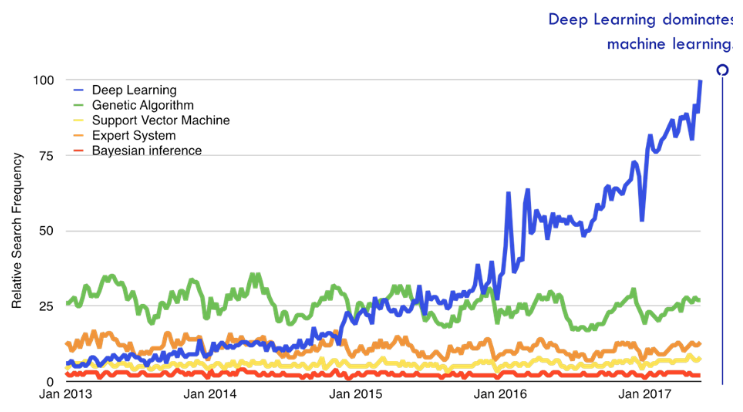
\includegraphics[scale=0.5]{images/deep-learning.png}
            \caption[The growth of deep learning compared to other machine learning algorithms]{The growth of deep learning compared to other machine learning algorithms \cite{leepdearning}}
            \label{fig:11}
        \end{figure}
        \par
        \par
        In the field Reinforcement Learning (RL), where tasks are learnt via trial-and-error by letting an agent
        interact with its environment, the same problem with handcrafted features exists. RL techniques rely on
        an internal representation of the state of the environment. This representation has to be derived from the
        agents percepts of the environment, which is most commonly done via handcrafted features. Therefore
        the applications of RL were limited to toy examples with a very low-dimensional state-space or to examples where the state-space could be thoroughly described via manually created features. Inspired by the
        advancements made in the field of deep learning, the subfield deep reinforcement learning emerged. As
        with deep learning in a supervised setting, a deep RL method also works directly on raw input instead
        of handcrafted features. Despite the young age of deep RL, several successful applications have already
        showed its power\cite{mnih2015humanlevel}\cite{DBLP:journals/corr/LevineFDA15}, among which AlphaGo is probably the best-known example \cite{deepGO}.
        \par
        This thesis will try to take even a step  further. While the vast majority of the newly developed deep
        RL methods were only tested on simple, basic simulations, it is reasonable to think that modern games, with complex strategies can also greatly benefit from deep RL techniques. However applying such methods
        involves many new challenges like e.g. dealing with huge state size and extremely long network convergence. This is exactly what is investigated
        in this thesis. More specifically the feasibility of the technique of Deep Q-Learning (DQL) \cite{mnih2015humanlevel} in complex and modern video games.

	\section{Problem Statement}
	    The main problem that will be discussed on this thesis is whether our new proposed method (Adam-DQL) is viable to solve complex video games. Specific research questions include:
        \begin{enumerate}
            \item How can the function that maps the in-game images into $Q$-values be determined?
            \item How can the desired function be represented?
            \item How viable is deep Q-learning to solve complex video games?
            \item Is it possible to improve techniques proposed by Deepmind using a better optimizer(Adam)?
            \item Is it possible to leverage the learning capabilities of Adam-DQL by adding policy improvement strategies such as partial training and demonstrations? 
    \end{enumerate}
        The secondary research questions are :
        \begin{enumerate}
            \item How can a general deep Q-learning implementation be developed ?
            \item What is the best structure of the software framework to allow seamless and efficient experiment? 
        \end{enumerate}
	    
%MODEL ASSUMPTIONS
	\section{Objectives}
	    The main objective of this thesis is to experimentally verify our method according to our problem statement. Listed below are the outline of our main objective in this thesis:
	    \begin{enumerate}
	    \item Develop a mathematical model, represented as directed acyclic graph, which maps a sequence of image to a vector of $Q$-values for each action. 
	    \item Develop a modified deep-Q learning technique using Adam optimizer.
        \item Develop a framework to allow an agent to interact with game environment.
        \item Implement the modified deep Q-learning for game environment.
        \item Describe and Interpret the results.
         \end{enumerate}
        To achieve the objectives described above, This thesis proposed several methods, which is listed below:
        \begin{enumerate}
        \item Review related research and literature.
        \item Develop a new deep learning algorithm, Adam-DQL, which consist of:
            \begin{enumerate}
            \item Modelling general video game as a Markov Decision Process.
            \item Deriving the Bellman optimality equation.
            \item Designing a neural network to approximate the $Q$-function.
            \item Deriving the loss function and gradient approximate equation.
            \item Implement a training algorithm for neural network based on DQN and Adam optimizer. 
            \item Address stability issues of Adam-DQL (partial training and demonstrations).
            \end{enumerate}
        
        \item Develop a software framework to interact with game environment, which consist of:
            \begin{enumerate}
            \item Implement Adam-DQL in Python.
            \item Modify and prepare few game environments to suit Adam-DQL testing requirements.
            \end{enumerate}
        
        \item Experimentally verify the capability of Adam-DQL, which consist of:
            \begin{enumerate}
            \item Train the neural network for a sample game.
            \item Describe and Interpret the Results.
            \end{enumerate}
        \end{enumerate}
        
   
		

	\section{Restrictions and Assumptions}
	    Since Adam-DQL is developed to create a general AI without any handcrafted features, Adam-DQL should work with every games, as long as it follows the restrictions and assumptions explained below:
        \begin{enumerate}
         \item The game environments are limited to the 1st stage only. This is more of a choice rather than a limitation. This choice comes from the fact that most games are designed to have an introductory stage, a stage that utilize every gameplay elements albeit being relatively simple. By restricting the scope to this introductory stages, the system can accommodate more gameplay concepts. Making the experiment much more accurate.
        \item Game environments can be stochastic. This assumption comes from the fact that generally, there's some random elements on games. Repeating the same action over and over again won't always produce the same result on these kind of games. By taking into account this stochastic elements, a more general, model-free method can be developed. 
        \item The Game has a constant amount of possible actions.
        This is a direct result of using output of a neural network to approximate the $Q$-function. A non constant amount of possible actions means the neural network has a non-constant output size. This is impossible since Neural networks structure is constant. An example of a game that doesn't have this constant action property is chess.
        \item The samples taken as minibatch in our training data are independent and identically distributed. This is the main requirement of using any stochastic/minibatch neural-network optimizer.
        \item The inputs for our neural network are taken from raw pixels and RAM(memory) only. This assumption allows the development of a system that is model-free, and can be used for general games with small to no modification.
        \item The interface layout for the game doesn't change overtime (static). Since adam-DQN's input is only raw pixels, it's not possible to accommodate a game that has changing game layout. Having a changing layout means the same position on the input might not represent the same thing overtime. This will create a noise in the training data and prevent the neural network to converge.
        \end{enumerate}
	
	\section{Benefits}
	There are several benefits of this research, both theoretical and practical, including:
	\subsection{Theoretical Benefits}
	\begin{enumerate}
	    
        \item
        Introduced new algorithm for higher-scale deep reinforcement learning in games. This will give an idea about how deep reinforcement learning with some modifications is highly usable in real world use case.
        \item Helps future researchers develop or compare various AIs by using software framework introduced in this thesis.
        \item A proof of concept that Demonstration, a technique used for robotics, can be applied to help solve complex games.
	    \item Introduced a new policy improvement technique called partial training, which kickstarts agent's reward for harder games.
	\end{enumerate}
	\subsection{Practical Benefits}
	\begin{enumerate}
        \item
        Allows the creation of general AI for more complex games, regardless of the genre and gameplay elements.
	\end{enumerate}

	\section{Thesis Structure}
	The writing structure of this thesis is as detailed below:
	\begin{enumerate}
	    \item Chapter I describes the background, problem statement, objectives, restrictions, and methodology. 
	    \item Chapter II describes the reinforcement learning with an emphasis on Q-learning and $\epsilon$-greedy policy. First, reinforcement learning in general will be presented, then, an introduction to reinforcement learning problem as Markov Decision Process will follow. After that, there will be some brief explanation about classical Q-learning algorithm and its feasibility in huge or immense state spaces. This chapter will be closed with an explanation of a classic problem in reinforcement learning, the exploration-exploitation dilemma. As well as $\epsilon$-greedy, an \textit{almost} greedy algorithm that solves the exploration-exploitation dilemma.
	    \item Chapter III describes the artificial neural networks, deep neural networks and deep learning technique. This chapter will start by explaining the underlying idea of artificial neural networks and convolutional neural networks. Then, it will be followed by the structural extension of artificial neural network, the deep neural networks. After that, there will be some quick introduction about how to train a neural network, as well as various optimizer (convex/nonconvex optimization algorithms). This chapter will be closed with an explanation of deep Q-learning, a method that combines reinforcement learning and deep neural networks.
	    \item Chapter IV contains implementation of deep Q-learning and the architecture of the whole learning system. This thesis propose a new modified algorithm called Adam-DQL that will be explained in this chapter. After that, the general structure of our framework will be described in detail. This chapter will also explain the structure of our neural network and every linearity (activation function) it uses. In this chapter we will also explain our state representation and our raw data input. 
	    \item Chapter V describes the various experiments and results for a sample game. This chapter will go even deeper into the selection of the framework architecture. There will be some experiment to test how well Adam-DQL performs in more modern games. However as explained earlier, Adam-DQL method should work for every game on the same platform with minimal to no changes. There will be some in-depth explanation about the results, as well as some comparison of Adam-DQL to other newly developed machine-learning algorithms.
	    \item Chapter VI summarizes achieved results, draw conclusions and proposes directions for further research.
	\end{enumerate}

%=================================CHAPTER II=========================================

\chapter{REINFORCEMENT LEARNING}
\thispagestyle{fancy}


%==================================================================================
	\section{Introduction}
        Reinforcement learning (RL) is the one of the most researched areas in artificial intelligence and
        machine learning, nowadays. In this approach an agent (also called a learner) is learning by interactions with a (possibly uncertain) environment. The agent learns what to do (how to map observed percepts to actions) to maximize (possibly discounted) cumulative reward, a.k.a reinforcement signal. The agent does not know, \textit{a priori}, what action to make, but has to explore (by trial-and-error) to understand which action provides the highest reward over the time by trial and error. Reinforcement learning consists in learning from a sequence of observed states, performed actions and received rewards.
		\par
		There are few differences when comparing reinforcement learning to supervised learning - the most popular learning paradigm studied in machine learning:
		\begin{itemize}
		    \item Supervised learning consists in learning from examples provided by an external supervisor, whereas in reinforcement learning an agent learns from its own experience (the task is defined in such way that a predefined dataset of examples is hard or even impossible to get, as opposed to the supervised learning). In other words, when it comes to committed error, a supervised learning agent knows exactly what it should have done, while a reinforcement learning agent only knows that an action was incorrect (and eventually to what extent it was incorrect).
		    \item Reinforcement learning has to deal with exploration-exploitation dilemma (described later in this section), while there is no such dilemma in supervised learning.
		    \item Reinforcement learning involves delayed rewards, while in supervised learning rewards are known immediately.
		    \item In supervised learning, the evaluation of the system is separated from the learning phase, whereas in reinforcement learning evaluation phase is usually done simultaneously with learning - reinforcement learning is, usually, on-line learning, while supervised learning is, typically, off-line learning.
		\end{itemize}
		
	\section{Markov Decision Process} \label{sec:21}
	    Reinforcement learning can be formulated as a class of Markov Decision Process (MDP). An MDP is a discrete-time, stochastic control process, defined as a tuple ( $S$, $A$, $P$, $R$, $\gamma$ ), in which:
	    \begin{itemize}
	        \item $S$ is a finite set of states ($s_t \in S$, where $s_t$ is state observed at (discrete) time $t$),
	        \item $A(s_t )$ is a finite set of possible actions in state $s_t$ ($a_t \in A(s_t ), A(s) \subset A$, where $a_t$ is action executed at time $t$),
	        \item $P (s, a, s') = P(s_{t+1}=s'|s_0, a_0, s_1,..., s_{t-1}, a_{t-1}, s_t=s, a_t=a) = P(s_{t+1}=s'|s_t=s,a_t=a)$ is the probability, that executing action $a$ in state $s$ at time $t$ will lead to state $s'$ at time $t + 1$,
	        \item $R(s, a)$ is function describing the immediate (or expected immediate) reward for taking action $a$ in state $s$,
	        \item $\gamma$ is the discount factor, which denotes the difference in priorities between the immediate reward and future rewards. A reward received n time steps ahead is worth $\gamma^{  n - 1 }$ times less than the same reward obtained immediately ( $\gamma \in (0, 1]$ ).
	    
	    \end{itemize}
	    \par
        The reinforcement learning problem is such MDP where $R$ or $P$ are unknown, which means the agent has to learn how an action is good (the reward function), and where his actions lead (the transition probabilities). The agent follows policy that is, in general, a mapping from states to probabilities of executing each (possible) action $(\pi : S \to A)$. The policy could be deterministic, and depend only on the state, $\pi(s)$, or stochastic, $\pi(a|s)$, such that it defines a probability distribution over the actions, given a state.
        
    \section{Value Function}
        The objective of a RL agent is to choose a policy which maximizes the expected sum of rewards. The sum of rewards is called as the return, $G_t$ , which is given as,
        \begin{equation*}
            G_t=r_t+r_{t+1}+r_{t+2}+...+r_{N}
        \end{equation*}
        where $N$ denotes the end of an episode, $t$ is the time index.
        However, in most cases, the environment for RL agent is stochastic, meaning there's a degree of uncertainty whether the agent will get the same reward if we take the same action in the future. Therefore it's common to use the discounted future reward, which incorporates $\gamma$ into the reward equation, which gives:
        \begin{equation*}
            G_t=r_t+\gamma r_{t+1}+\gamma^2 r_{t+2}+...=\sum_{k=0}^{\infty}\gamma^k r_{t+k}
        \end{equation*}
        \par
        In order to be able to decide what action to take at a particular instant, it is important for the agent to know how good it is for the agent to be in a particular state. A way of measuring the "goodness" of a state is the \textit{value function}. It is defined as the expected sum of rewards that the agent will receive while following a particular policy $\pi$ from a particular state s. The value function, $V_\pi(s)$ for policy $\pi$ is given by
        
        \begin{equation*}
            V_\pi (s)=\mathbb{E}_\pi (G_t|s_t=s) = \mathbb{E}_\pi (\sum_{k=0}^{\infty}\gamma^k r_{t+k } | s_t=s )
        \end{equation*}
        
        Similarly, an \textit{action value function}, also known as the $Q-function$, can be defined which is the expected sum of rewards while taking action a in state s and, thereafter, following policy $\pi$. The action value function, $Q_\pi (s, a)$ is given by
        
        \begin{equation} \label{eq:21}
            Q_\pi (s,a)=\mathbb{E}_\pi (G_t|s_t=s,a_t=a) = \mathbb{E}_\pi (\sum_{k=0}^{\infty}\gamma^k r_{t+k } | s_t=s,a_t=a )
        \end{equation}
        
        It is unusual that an agent receives accurate information about reward directly after performing each action, most of the time a future cumulative reward is delayed. For example, in any board game, it is hard to estimate how a single move will affect the overall game state. In such case, an agent may not receive any reward information until the end of the game. Thus, the learner must propagate the delayed reinforcement to previous states and actions that (implicitly) caused this reinforcement. This is known as \textit{temporal credit assignment problem}.
        
    \section{Bellman Equation}\label{sec:24}
        The Bellman equations formulate the problem of maximizing the expected sum of rewards
        in terms of a recursive relationship of a value function. A policy $\pi$ is considered better than
        another policy $\pi'$ if the expected return of that policy is greater than $\pi'$ for all $s \in S$, which
        implies, $V_\pi (s) \geq V_\pi' (s)$ for all $s \in S$. Thus, the optimal value function, $V_*(s)$ can be defined
        as,
        
        \begin{equation*}
            V_* (s)= \max V_\pi(s), \forall s \in S.
        \end{equation*}
        Similarly, the optimal \textit{action value function}, $Q_*(s,a)$ can be defined as,
        \begin{equation*}
            Q_* (s,a)= \max Q_\pi(s,a), \forall s \in S, a \in A.
        \end{equation*}
        Also, for an optimal policy, the following equation can be written,
        \begin{equation} \label{eq:22}
            V_* (s)= \max_{a \in A} Q_{\pi*}(s,a)
        \end{equation}
        Expanding equation (\ref{eq:22}) with (\ref{eq:21}),
        \begin{equation} \label{eq:23}
            \begin{split}
                V_*(s) &=\max_{a}\E_{pi*}(G_t|s_t=s,a_t=a) \\
                & = \max_{a}\E_{pi*}(\sum_{k=0}^{\infty}\gamma^k r_{t+k } | s_t=s,a_t=a ) \\
                & = \max_{a}\sum_{s'}p(s'|s,a)[R(s,a,s')+\gamma V_*(s')]
            \end{split}
        \end{equation}
        Equation (\ref{eq:23}) is known as the Bellman optimality equation for $V_*(s)$. The Bellman optimality equation for $Q_∗$ is
        \begin{equation*}
            \begin{split}
                Q_*(s,a)& =\E(r_t+\gamma \max_{a'}Q_*(s_{t+1},a')|s_t=s,a_t=a) \\
                & = \sum_{s'}p(s'|s,a)[R(s,a,s')+\gamma\max_{a'}Q_*(s',a')]
            \end{split}
        \end{equation*}
        
        If the transition probabilities and the reward functions are known, the Bellman optimality equations can be solved in an iterative fashion. This approach is known as \textit{Dynamic programming}. The algorithms which assume these probabilities to be known or estimate them online are collectively known as \textit{model-based} algorithms.
        \par
        But for most other algorithms, they assume the probabilities are not known and they estimate the policy and value function by performing rollouts on the system. These methods are known as model-free algorithms (Section \ref{sec:25}). Monte Carlo and temporal difference are the most common model-free algorithms used.
    
    \section{Model-Free Methods}\label{sec:25} 
            Model-free methods can be applied to any reinforcement learning problem since they do not
        require any model of the environment. Most model-free approaches either try to learn a value
        function and infer an optimal policy from it (Value function based methods) or directly search
        in the space of the policy parameters to find an optimal policy (Policy search methods).
        Model-free approaches can also be classified as being either \textit{on-policy} or \textit{off-policy}. On-policy
        methods use the current policy to generate actions and use it to update the current policy
        while off-policy methods use a different exploratory policy to generate actions as compared
        to the policy which is being updated. The following subsections look at various model-free
        algorithms used, both value function based and policy search methods.
        \subsection{Monte Carlo Methods}
                Monte Carlo methods work on the idea of generalized policy iteration (GPI). The GPI is an
        iterative scheme and is composed of two steps. The first step tries to build an approximation
        of the value function based on the current policy, known as the \textit{policy evaluation} step. In the
        second step, the policy is improved with respect to the current value function, known as the
        \textit{policy improvement step}. In Monte Carlo methods, to estimate the value function, rollouts
        are performed by executing the current policy on the system. The accumulated reward over
        the entire episode and the distribution of states encountered is used to form an estimate of
        the value function. The current policy is then estimated by making it directly greedy with
        respect to the current value function. Using these two steps iteratively, it can be shown that
        the algorithm converges to the optimal value function and policy. Though Monte Carlo methods are straightforward in their implementation, they require a large number of iterations for
        their convergence and suffer from a large variance in their value function estimation.
        \subsection{Temporal Difference}
        Temporal difference (TD) builds on the idea on the GPI but differs from the Monte Carlo
        methods in the policy evaluation step. Instead of using the total accumulated reward, the
        methods calculate a temporal error, which is the difference of the new estimate of the value
        function and the old estimate of the value function, by considering the reward received at the
        current time step and use it to update the value function. This kind of an update reduces the
        variance but increases the bias in the estimate of the value function. The update equation
        for the value function is given by:
        
        \begin{equation}\label{eq:24}
            V(s) \gets V(S) + \alpha[r+\gamma V(s') - V(s)]
        \end{equation}
        
        where, $\alpha$ is the learning rate, $r$ is the reward received at the current time instant, $s'$ is the new state and $s$ is the old state. Thus, temporal difference methods update the value function at each time step, unlike the Monte Carlo methods which wait till the episode has ended to update the value function.
        
        \subsection{Q-Learning} \label{sec:253}
            Watkins \cite{Watkins:1989} introduced an off-policy temporal difference algorithm known as $Q$learning.$Q$-learning is a model-free, temporal difference algorithm to learn action-value function for any Markov decision process. $Q$-learning is an off-policy method. It means that it learns the optimal strategy independently of the agent's behavior, in contrast to on-policy methods, which learn the policy being followed by the agent (including non-greedy, exploration steps). $Q$ learning is based on Bellman equation (Section \ref{sec:24}), thus, by applying temporal difference update (Equation \ref{eq:24}) into Bellman equation (Equation \ref{eq:21}), resulting in:
            \begin{equation}\label{eq:25}
                Q(s,a) \gets Q(s,a) + \alpha[R(s,a)+ \max_{a' \in A(s)} Q(s',a')-Q(s,a)], 
            \end{equation}
            where all of the parameters have the same meaning as (Equation \ref{eq:24}) and (\ref{eq:21}).
            \par
            In the most straightforward implementation of $Q$-learning, the state-action values are stored in a look-up table (LUT). Q-learning uses Equation (\ref{eq:25}) to iteratively update the value of $Q(s, a)$ by updating appropriate values in table $Q[S, A]$ where $S$ is a set of possible states and $A$ is a set of all possible actions. During the learning $Q[s, a]$ represents current estimate of $Q_*(s, a)$, where $Q_*$ is the optimal state-action value.
            $Q$-learning algorithm with LUT algorithm is presented in Algorithm \ref{alg:1}:
            \par
            \begin{algorithm}[H]\label{alg:1}
                For each possible state-action pair initialize table $Q[s,a]$ to zero\\
                Observe current state $s$\\
                \While{stop condition not satisfied}{
                Select action $a$ (according to utility function for state $s$): \\
                    $a= \argmax_{a'} Q(s',a')$ \\
                Execute action $a$\\
                Receive immediate reward $r$\\
                Observe new state $s'$\\
                Update Table Entry $Q[s,a]$ using the update rule: 
                    $Q(s,a) \gets Q(s,a) + \alpha[R(s,a)+ \max_{a' \in A(s)} Q(s',a')-Q(s,a)],$ \\
                Assume $s'$ as new state $s$\\
                }
            
            \caption{Q Learning algorithm with LUT}
            \end{algorithm}
            \vspace{5mm}
            
            
            In real world problems, keeping table $Q[S, A]$ for each action in each state is not possible,
            because the state space is too large to consider explicitly each of the states. One has to use
            approximation function  $\hat{Q}(s,a)$ instead, which advantage is that it also generalizes the acquired
            knowledge over non-visited states. Such a function approximator is also a compromise between
            the quality of approximation and the time necessary to learn.
            The state is represented as a set of features $f_1 , f_2 , ..., f_n$,  where the number of features is
            significantly lower than the number of possible states. The $Q$-function is parametrized by the
            vectors of parameters $\theta$. During the learning process, only $\theta = (\theta_1 , \theta_2 , ..., \theta_n )$ parameters are subjected to learning. According to the Widrow-Hoff's \cite{Sutton81towardsa} rule, parameters should change along
            the gradient in order to minimize the overall loss $L_\theta$, that is, the MSE (Mean Squared Error) of $Q$ :
            \begin{equation*}
                L_\theta=\frac{1}{2}(\hat{Q}(s,a)-Q(s,a))^2
            \end{equation*}
            The update rule for $\theta$ parameters in Q learning is as follows :
            \begin{equation*}
                \theta_i \gets \theta_i - \alpha \frac{\partial{L_\theta(s,a)}}{\partial{\theta_i}}=\theta_i - \alpha(\hat{Q}(s,a)-Q(s,a)) \frac{\partial{\hat{Q}(s,a)}}{\partial{\theta_i}}
            \end{equation*}
            Expanding it with (Equation \ref{eq:25})    
            \begin{equation*}
                \theta_i \gets \theta_i - \alpha(\hat{Q}(s,a)-(R(s,a)+ \max_{a' \in A(s)} Q(s',a')) \frac{\partial{\hat{Q}(s,a)}}{\partial{\theta_i}}
            \end{equation*}
            \par
            The approximator $\hat{Q}(s,a)$ could be any function approximator, with the simplest one being linear approximator (linear combination) of state features with factors $\theta_1,\theta_2,\theta_3,..,\theta_n$:
            \begin{equation*}
                \hat{Q}(s,a)=\theta_1 f_1(s)+ \theta_2 f_2(s) + ... + \theta_n f_n(s)
            \end{equation*}
            
            However, most of the real world problems require a more complex, nonlinear approximator, with the most popular one being \textit{artificial neural network}. This approach has been used successfully in many previous studies \cite{bingqiang} \cite{Dini12combiningq-learning}\cite{touzet}. Input to such a neural network is encoded state and output is Q-value for particular action. Actually, there are at least two options for neural network outputs: neural network could have number of outputs equal to the number of overall possible actions or there could be separated neural network for each action, where each neural network have only one output. This topic will be broadly discussed in Section \ref{sec:3}
            
            
            
            \section{$\epsilon$-greedy policy} \label{section:26}
                $\epsilon$-greedy policy handles the exploration-exploitation dilemma. A greedy algorithm is an algorithm
            that always takes whatever action seems to be the best according to the action-value function $Q$.
            \par
            A greedy agent might fall into a local optima. The $\epsilon$-greedy algorithm is almost a greedy algorithm,
            because it exploits the best available option, but once in a while, it explores the other available
            options. Using this strategy, either a random action is selected with probability $\epsilon$ or an action
            defined by agent current policy $\pi$ is selected with probability 1 - $\epsilon$ .
            \par
             Epsilon can be fixed during the learning, but annealing it often leads to better results. For
            example, the agent can initially start with $\epsilon$ = 1 (full exploration - always select a random action),
            then, progressively with each game played, $\epsilon$ is decreased linearly towards $\epsilon_f$ value, reaching it
            after $K$ played episodes. By using linear annealing of $\epsilon$, with each successive episode, the agent
            uses an action provided by $Q$-function more frequently (agent is moving forwards to almost full
            exploitation), ending with only few percent of random actions (e.g., $\epsilon_f = 0.01$, which means that
            one in one hundred actions is selected by random) after a predefined number of episodes.
            

%=================================CHAPTER III=========================================

\chapter{DEEP LEARNING AND DEEP NEURAL NETWORKS}
\thispagestyle{fancy}

	In recent years, the popularity of deep learning has increased enormously in the machine learning
community. Deep learning tries to model and extract high-level abstraction features in data using
complex, multi-layer models and non-linear transformations. Deep learning methods are used
in both supervised and unsupervised learning. In contrast to shallow learning algorithms, deep
learning algorithms are distinctive by the number of transformations each signal encounter during
its propagation from the input to the output. There are many motivations to explore deep
algorithms:
\begin{itemize}
    \item the ability to learn complex functions,
    \item the ability to learn high-level, hierarchical abstractions,
    \item the ability to learn from a very large set of training data, and
    \item the ability to learn from unlabeled data.
\end{itemize}
Deep learning was successfully applied in multiple fields such as speech recognition \cite{socher}, image
recognition and classification \cite{Krizhevsky:2017:ICD:3098997.3065386}, natural language processing \cite{socher} and many other tasks in
machine learning \cite{dengli}. In all of these studies, the performance of the resulting algorithm was better
than other machine learning approaches to these problems.

\section{Artificial Neural Networks} \label{sec:3}
    One of the most common approaches in deep learning involves using artificial neural networks
    (ANN). Artificial neural networks are inspired by biological neural networks (especially model of
    a human brain) and are used to estimate the value of complex functions, which could depend on
    numerous inputs.
    Artificial neural network, illustrated in Figure \ref{fig:31} , is a system of connected artificial neurons,
    which are mathematical functions imitating biological neurons. Artificial neuron receives one
    or more signals x as an input (referencing biological neuron's dendrites) and transforms them
    to produce an output (representing biological neuron's axon). Usually, this transformation is a
    weighted sum of all inputs processed at the end by a non-linear activation function $\phi$. Neural
    output for a given input vector $x$ is defined by the following formula:
    \begin{equation} \label{eq:31}
        f(x)=\phi(\sum_i w_i x_i + b_i)
    \end{equation}
    where $w_i$ is the weight of input $i$, $x_i$ is the actual input and $b_i$ represent biases.
    \par
    \begin{figure}[H]
        \centering
        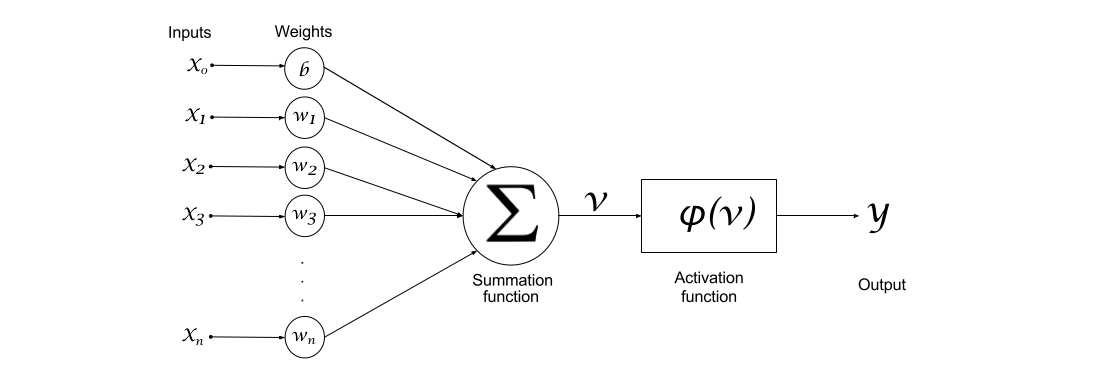
\includegraphics[scale=0.3]{images/aneuron.png}
        \caption{Artificial Neuron}
        \label{fig:31}
    \end{figure}
    
    \subsection{Non Linearity/ Activation Function}
    The capacity of the neural networks to approximate any functions, especially non-convex, is directly the result of the non-linear activation functions, referred as $\phi$ in the last section.  takes a vector and performs a certain fixed point-wise operation on it. There are three main activation functions:
    \vspace{5mm}
    \par \noindent
    \textbf{Sigmoid} The Sigmoid non-linearity has the following mathematical form:
    \begin{equation*}
        \phi=\sigma(x)=\frac{1}{1+e^{-x}}
    \end{equation*}
        It takes a real value and squashes it between 0 and 1. However, when the neuron's activation saturates at either tail of 0 or 1, the gradient at these regions is almost zero. Thus, the backpropagation algorithm fail at modifying its parameters and the parameters of the preceding neural layers.
    \vspace{5mm} \par \noindent
    \textbf{Hyperbolic Tangent} The TanH non-linearity has the following mathematical form
      \begin{equation*}
        \phi=2\sigma(2x)-1
    \end{equation*}
        It squashes a real-valued number between -1 and 1. However it has the same drawback as sigmoid.
    
    \vspace{5mm} \par \noindent
    \textbf{ReLU (Rectified Linear Unit)} The ReLU has the following mathematical form
    \begin{equation*}
        \phi=max(0,x)
    \end{equation*}
        The ReLU has become very popular in the last few years, because it was found to greatly
        accelerate the convergence of stochastic gradient descent compared to the sigmoid/tanh
        functions due to its linear non-saturating form. In fact, it does not suffer from the vanishing or exploding gradient. An other advantage is that it involves cheap operations compared to the expensive exponentials. However, the ReLU
        removes all the negative informations and thus appears not suited for all datasets and architectures.
    
    \subsection{Convolutional Layers}
    \subsubsection{Spatial Convolution Layer}
    Regular Neural Networks, only made of linear and activation layers, do not scale well to full images. For instance, images of size $3 \times 224 \times 224$ (3 color channels, 224 wide, 224 high) would necessitate a first linear layer having 3  $224 \times 224 + 1 = 150$, 129 parameters for a single neuron (e.g. output). Spatial convolution layers take advantage of the fact that their input (e.g. images or feature maps) exhibits many spatial relationships. In
    fact, neighboring pixels should not be affected by their location within image. Thus, a
    convolutional layer learns a set of $N_k$ filters $F = f_1 , ..., f_{N_k}$ , which are convolved spatially
    with input image $x$, to produce a set of $N_k$ 2D features maps $z$:
    
    \begin{equation*}
        z_k=f_k * x
    \end{equation*}
    
    where $*$ is the convolutional operator. When the filter correlates well with a region of the
    input image, the response in the corresponding feature map location is strong. Unlike
    conventional linear layer, weights are shared over the entire image reducing the number of
    parameters per response and equivariance is learned (i.e. an object shifted in the input image will simply shift the corresponding responses in a similar way). Also, a fully connected layer can be seen as a convolutional layer with filter of sizes $1 \times 1 \times inputSize$.  
    \par
    It is important to highlight that a spatial convolution is not defined by the spatial size
    of the input feature maps (e.g. wide and high), neither by the size of the output feature
    maps, but by the number of filters (e.g. number of output channels), the properties of its
    filters (e.g. number of input channels, wide, high) and the properties of the convolution
    (e.g. padding, stride).
    \begin{figure}[H]
        \centering
        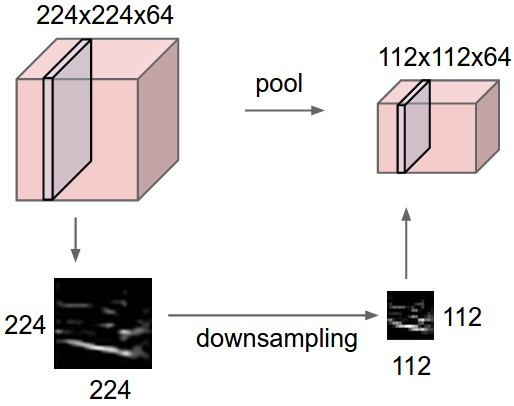
\includegraphics[scale=0.5]{images/spatialpooling.png}
        \caption[Spatial Pooling Operation]{The illustration of a spatial pooling operation in $2 \times 2$ regions by a stride of 2
        in the high direction, and 2 in the width direction, without padding.\cite{DBLP:journals/corr/CadeneTC16}}
        \label{fig:32}
    \end{figure}
    
    \subsubsection{Spatial Pooling}
            In Convolutional Neural Networks, a pooling layer is typically present to provide invariance
        to slightly different input images and to reduce the dimension of the feature maps (e.g.
        wide, high):
        \begin{equation*}
        p_R=P_{i \in R}(z_i)            
        \end{equation*}
        where $P$ is a pooling function over the region of pixels $R$. Max pooling is preferred as
        it avoids cancellation of negative elements and prevents blurring of the activations and
        gradients throughout the network since the gradient is placed in a single location during
        backpropagation.
        The spatial pooling layer is defined by its aggregation function, the high and width dimensions of the area where it is applied, and the properties of the convolution (e.g. padding,
        stride).
        
\section{Feed Forward Neural Networks}
    The most common architecture used in DNN is the \textit{Feed-Forward neural network}. Figure
    3 shows an example of a feed-forward neural network. In this framework, the neurons are
    arranged in layers. This architecture usually has three kinds of layers: an input layer, a few
    \textit{hidden layers} and an \textit{output layer}. The flow of information takes place from the input layer
    to the hidden layers and finally to the output layer which computes the final output. Each
    neuron in the different layers performs the same computation as shown in Equation \ref{eq:31} .
    \begin{figure}[H]
        \centering
        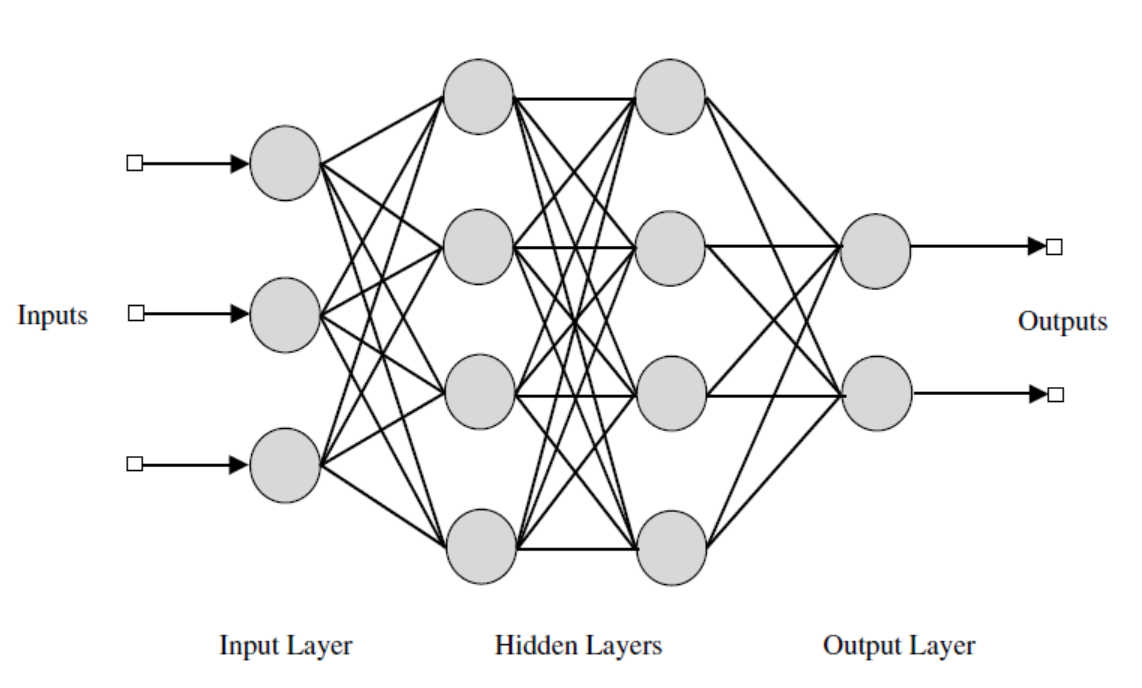
\includegraphics[scale=0.3]{images/ffnn.png}
        \caption[Feed Forward Neural Network]{Feed Forward Neural Network \cite{ffnn}}
        \label{fig:33}
    \end{figure}
    
\section{Deep Neural Networks}
        Traditional feedforward neural networks are considered to have the depth equal to the number of
    layers (i.e. the number of hidden layers plus 1, for the output layer). In many simple problems
    neural networks with depth 2 were successfully used, but there are many cases when single hidden
    layer is not enough. Solution to this problem is a deep neural network (DNN) - an artificial neural
    network with at least two hidden layers. The extra layers enable composition of features from
    lower layers, giving the potential of modeling complex, hierarchial features with a fewer units than
    in a shallow network. By providing sufficient amount of data to deep neural networks, it is often
    possible to learn better models than hand-coded features \cite{Krizhevsky:2012:ICD:2999134.2999257}.
    Before 2006 attempts at training deep architectures failed: training a deep feedforward neural network usually returns worse results than when using shallow architectures. Two papers \cite{Hinton:2006:FLA:1161603.1161605}\cite{Bengio:2006:GLT:2976456.2976476}, published in 2006, revolutionized deep architectures. The key principles in all
    of these papers were:
    \begin{itemize}
    \item unsupervised learning of representations is used to pre-train each layer,
    \item unsupervised training one layer at a time, using previously trained ones,
    \item supervised training to tune all layers together.
    \end{itemize}
    Deep neural networks are usually designed as basic feedforward networks, but in many recent
    studies deep learning architecture was created using convolutional deep neural networks (especially
    in image recognition and processing) \cite{DBLP:journals/corr/MnihKSGAWR13} \cite{mnih2015humanlevel}.
    
    \begin{figure}[H]
        \centering
        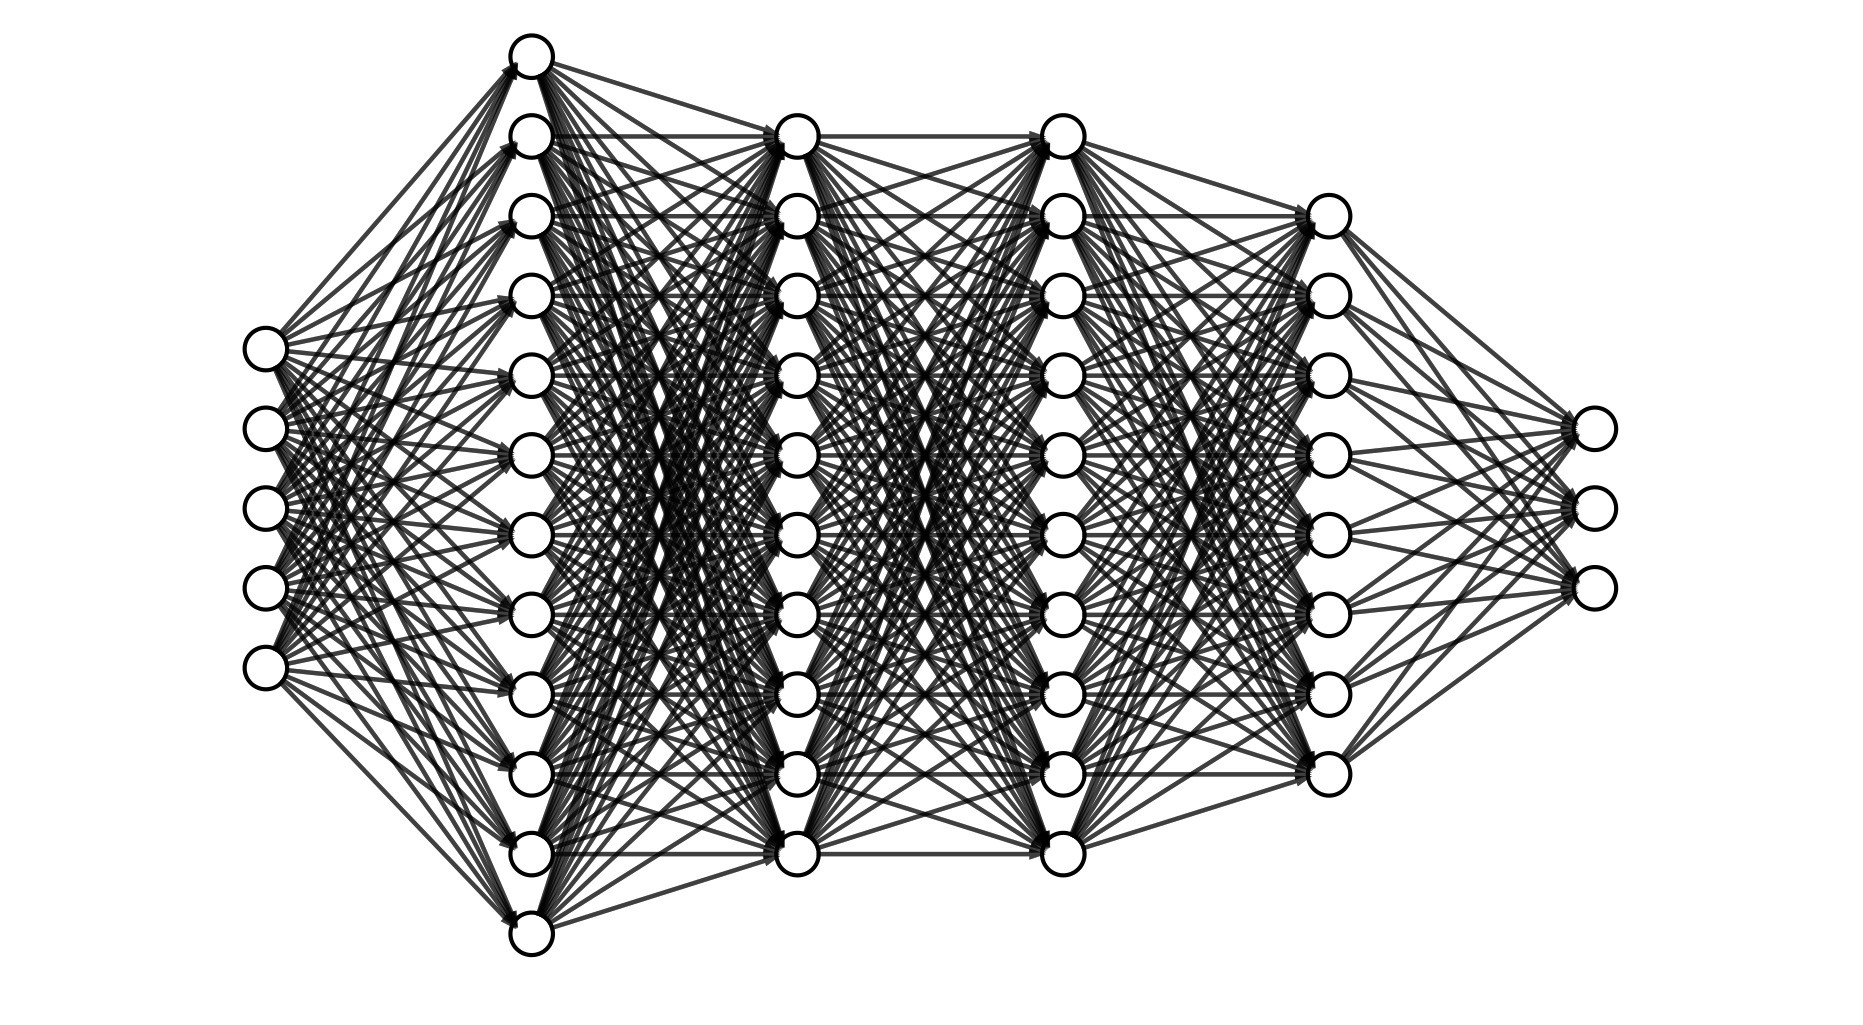
\includegraphics[scale=0.2]{images/dnn.png}
        \caption{Deep Neural Networks}
        \label{fig:34}
    \end{figure}
    
\section{Training Strategies/Methods}
    \subsection{Loss Function}
    To quantify the capacity of the network to approximate the ground truth
    labels for all training inputs, we define a loss function which takes as inputs the weights,
    biases, and examples from the training set. For instance, the loss could be the number
    of images correctly classified. Two most used loss functions to train deep neural networks are:
    
    \vspace{5mm}
    \par \noindent
    \textbf{Mean Squared Error (MSE)} MSE is a multi class loss formerly used to train neural
    networks.
    \begin{equation}
        Loss(x,y)= \frac{1}{n}\sum_i{|x_i-y_i|}^2
    \end{equation}
    with $x$ a vector of n predictions, and $y$ a binary vector full of 0 besides a 1 in the corresponding class dimension .
    
    \vspace{5mm}
    \par \noindent
    \textbf{Cross Entropy} Cross Entropy is a multi class loss which is nearly a better choice than MSE.
    \begin{equation}
        Loss(x,y)= -\sum_i y_i * log(\frac{e^{x_i}}{(\sum_j e^{x_j})})
    \end{equation}
    with $x$ a vector of n predictions, and $y$ a binary vector full of 0 besides a 1 in the corresponding class dimension .
   
    \subsection{Optimization}\label{sec:342}
    Once loss function for a neural network is decided, the training process is simply an (convex or non convex) optimization to minimize the value of the loss function. The idea in this approach is to start with a random initialization of the weights and calculate the output for a given input. the value of the loss function between the generated output and the actual output is used to update the weights of the network using an optimization algorithm. Since the weights are first updated of the output layer and then backpropagated into the network, the technique is known as \textit{backpropagation}.
    
    There are several optimization techniques commonly used in the training of neural networks, namely SGD (Stochastic Gradient Descent), Adagrad, RMSProp and Adam.
    
    The material on this subsection is taken from \cite{Goodfellow-et-al-2016}
    \subsubsection{Stochastic Gradient Descent (SGD)}
    Stochastic gradient descent (SGD) and its variants are probably the most used optimization algorithms for machine learning in general and for deep learning in particular. It is proven in  [Botton (1998)] that it is possible to obtain an unbiased estimate of the gradient by taking the average gradient on a minibatch of $m$ examples drawn i.i.d from the data-generating distribution.
    
        A crucial parameter for the SGD algorithm is the learning rate. Previously, we
    have described SGD as using a fixed learning rate $\epsilon$. In practice, it is necessary to
    gradually decrease the learning rate over time, so we now denote the learning rate
    at iteration $k$ as $\epsilon_k$ 
    This is because the SGD gradient estimator introduces a source of noise (the random sampling of
    $m$ training examples) that does not vanish even when we arrive at a minimum. By comparison, the true gradient of the total cost function becomes small and then
    become $0$ when we approach and reach a minimum using batch gradient descent, so batch gradient descent can use a fixed learning rate. A sufficient condition to guarantee convergence of SGD is that:
    
    \begin{equation}
        \sum_{k=1}^\infty \epsilon_k = \infty
    \end{equation}
    In practice, it is common to decay the learning rate linearly until iteration $\tau$:
    \begin{equation}
        \epsilon_k=(1-\alpha)\epsilon_0+\alpha \epsilon_\tau
    \end{equation}
    where $\alpha = \frac{k}{\tau}$. After iteration $\tau$, it is common to leave $\epsilon$ constant.
    The SGD algorithm is fully presented in Algorithm \ref{alg:2}:
 \vspace{5mm}
    \par
            \begin{algorithm}[H]\label{alg:2}
            \textbf{Require:} Learning Rate $\epsilon_1,\epsilon_2,...$ \\
            \textbf{Require:} Initial parameter $\theta$ \\
                $k \gets 1$ \\
                \While{stop condition not satisfied}{
                Sample a minibatch of $m$ examples from the training set {$x^{(i)},...x^{(m)}$} and corresponding targets $y^{(i)}$ \\
                Compute gradient estimate: $\hat{g} \gets \frac{1}{m} \nabla_\theta \sum_i L(f(x^{(i)};\theta),y^{(i)}) $ \\
                Apply update: $\theta \gets \theta- \epsilon_k \hat{g}$ \\
                $k\gets k+1$ \\
                }
            
            \caption{Stochastic Gradient Descent Update}
            \end{algorithm}

    
    
    \subsubsection{AdaGrad}
    The AdaGrad (Adaptive Gradient) algorithm, individually adapts the learning
    rates of all model parameters by scaling them inversely proportional to the square
    root of the sum of all the historical squared values of the gradient \cite{Duchi:2011:ASM:1953048.2021068}. 
    The parameters with the largest partial derivative of the loss have a
    correspondingly rapid decrease in their learning rate, while parameters with small
    partial derivatives have a relatively small decrease in their learning rate. The net
    effect is greater progress in the more gently sloped directions of parameter space.
    
        In the context of convex optimization, the AdaGrad algorithm enjoys some
    desirable theoretical properties. Empirically, however, for training deep neural
    network models, the accumulation of squared gradients from the \textit{beginning of
    training} can result in a premature and excessive decrease in the effective learning
    rate. AdaGrad performs well for some but not all deep learning models. AdaGrad algorithm is fully presented in Algorithm \ref{alg:3}:
 \vspace{5mm}
    \par
            \begin{algorithm}[H]\label{alg:3}
            \textbf{Require:} Learning Rate $\epsilon$ \\
            \textbf{Require:} Initial parameter $\theta$ \\
            \textbf{Require:} Small constant $\delta $ for numerical stability \\
                initialize gradient acculumation variable $r=0$ \\
                \While{stop condition not satisfied}{
                Sample a minibatch of $m$ examples from the training set {$x^{(i)},...x^{(m)}$} and corresponding targets $y^{(i)}$ \\
                Compute gradient estimate: $g \gets \frac{1}{m} \nabla_\theta \sum_i L(f(x^{(i)};\theta),y^{(i)}) $ \\
                Accumulate squared gradient: $r \gets r+g \bigodot g$ \\
                Compute update: $\Delta \theta \gets -\frac{\epsilon}{\delta+\sqrt{r}}\bigodot g.$ (Division and square root applied element-wise) \\
                Apply update: $\theta \gets \theta +\Delta \theta$\\

                }
            
            \caption{AdaGrad Update}
            \end{algorithm}

    
    
    \subsubsection{RMSProp}
    
        The RMSProp algorithm \cite{DBLP:journals/corr/abs-1207-0580} modifies AdaGrad to perform better in
    the nonconvex setting by changing the gradient accumulation into an exponentially
    weighted moving average. AdaGrad is designed to converge rapidly when applied to
    a convex function. When applied to a nonconvex function to train a neural network,
    the learning trajectory may pass through many different structures and eventually
    arrive at a region that is a locally convex bowl. AdaGrad shrinks the learning rate
    according to the entire history of the squared gradient and may have made the
    learning rate too small before arriving at such a convex structure. 
        RMSProp uses an exponentially decaying average to discard history from the extreme past so that
    it can converge rapidly after finding a convex bowl, as if it were an instance of the
    AdaGrad algorithm initialized within that bowl. RMSProp is shown in its standard form in Algorithm \ref{alg:4}:
 \vspace{5mm}
    \par
            \begin{algorithm}[H]\label{alg:4}
            \textbf{Require:} Learning Rate $\epsilon$, decay rate $\rho$ \\
            \textbf{Require:} Initial parameter $\theta$ \\
            \textbf{Require:} Small constant $\delta $ for numerical stability \\
                initialize gradient acculumation variable $r=0$ \\
                \While{stop condition not satisfied}{
                Sample a minibatch of $m$ examples from the training set {$x^{(i)},...x^{(m)}$} and corresponding targets $y^{(i)}$ \\
                Compute gradient estimate: $g \gets \frac{1}{m} \nabla_\theta \sum_i L(f(x^{(i)};\theta),y^{(i)}) $ \\
                Accumulate squared gradient: $r \gets \rho r+(1-\rho)g \bigodot g$ \\
                Compute update: $\Delta \theta \gets -\frac{\epsilon}{\delta+\sqrt{r}}\bigodot g.$ (Division and square root applied element-wise) \\
                Apply update: $\theta \gets \theta +\Delta \theta$\\

                }
            
            \caption{RMSProp Algorithm Update}
            \end{algorithm}

            
    \subsubsection{Adam}
        Adam \cite{DBLP:journals/corr/KingmaB14} is yet another adaptive learning rate optimization
        algorithm and is presented in Algorithm \ref{alg:5}. The name "Adam" derives from
        the phrase "adaptive moments". In the context of the earlier algorithms, it is
        perhaps best seen as a variant on the combination of RMSProp and momentum
        with a few important distinctions. First, in Adam, momentum is incorporated
        directly as an estimate of the first-order moment (with exponential weighting) of
        the gradient. The most straightforward way to add momentum to RMSProp is to
        apply momentum to the rescaled gradients. The use of momentum in combination
        with rescaling does not have a clear theoretical motivation. Second, Adam includes
        bias corrections to the estimates of both the first-order moments (the momentum
        term) and the (uncentered) second-order moments to account for their initialization
        at the origin. RMSProp also incorporates an estimate of the
        (uncentered) second-order moment; however, it lacks the correction factor. Thus,
        unlike in Adam, the RMSProp second-order moment estimate may have high bias
        early in training. Adam is generally regarded as being fairly robust to the choice
        of hyperparameters, though the learning rate sometimes needs to be changed from
        the suggested default.
         \vspace{5mm}
        \par
            \begin{algorithm}[H]\label{alg:5}
            \textbf{Require:} Step size $\epsilon$ \\
            \textbf{Require:} Initial parameter $\theta$ \\
            \textbf{Require:} Small constant $\delta $ for numerical stability \\
            \textbf{Require:} Exponential decay rate $\rho_1$ and $\rho_2$ (Suggested defaults: 0.9 and 0.999)
                initialize 1st and 2nd moment variables $s=0, r=0$ \\
                initialize time step t=0\\
                \While{stop condition not satisfied}{
                Sample a minibatch of $m$ examples from the training set {$x^{(i)},...x^{(m)}$} and corresponding targets $y^{(i)}$ \\
                Compute gradient estimate: $g \gets \frac{1}{m} \nabla_\theta \sum_i L(f(x^{(i)};\theta),y^{(i)}) $ \\
                $t \gets t+1$\\
                Update biased first moment estimate: $s \gets \rho_1 s+ (1-\rho_1)g$\\
                Update biased second moment estimate: $r \gets \rho_2 r+(1-\rho_2)g \bigodot g$\\
                Correct bias in first moment: $\hat{s} \gets \frac{s}{1-\rho_1^t}$\\
                Correct bias in second moment: $\hat{r} \gets \frac{r}{1-\rho_2^t}$\\
                Compute update: $\Delta \theta \gets -\frac{\epsilon}{\delta+\sqrt{r}}\bigodot g.$ (Division and square root applied element-wise) \\
                Apply update: $\theta \gets \theta +\Delta \theta$\\

                }
            
            \caption{The Adam algorithm}
            \end{algorithm}

\section{Deep Q-learning}
    \label{sec:dql}
    $Q$-learning (Section \ref{sec:253}) has been a widely used algorithm for model-free reinforcement learning. However, reinforcement learning is known to be unstable (or even to diverge) when a nonlinear function approximator such as a neural network is used to represent the Q-function \cite{Tsitsiklis97ananalysis}. This instability is caused by correlations between succeeding observations, the fact, that small updates of $Q$-function
    may substantially change policy, and the correlations between the $Q$-value and target values. There's a breakthrough for this problem, proposed by \cite{mnih2015humanlevel}, it was shown that $Q$-learning could be used with Deep Neural Networks and the algorithm showed human level performance on seven Atari 2600 games using only raw image pixels as the input. The key points of this paper is an mechanism called \textit{experience replay}.
    \par
    \subsection{Experience Replay and Minibatches Learning}
         To inhibit first of this issues, biologically-inspired mechanism called experience
        replay is used \cite{Lin1992}. In this idea, the agent can experience the effects of its actions without actually executing them. Data used to learning is randomly sampled at each step from memory of agent's previous transitions, what removes the correlation in the sequence of training examples and smooths the training distribution over many past behaviors, thus reducing oscillations and divergence of the learning process. Another advantage of this mechanism is reusing single experience in many weights updates, which allows for greater data efficiency \cite{mnih2015humanlevel}. Note that using experience replay implies
        off-policy learning (see Section \ref{sec:253}), because current parameters are different than the ones used to generate experience sample. 
    \par
         To perform experience replay, agent's transitions experience at each time step t are stored in dataset $D$ as a tuple $ e_t = (s_t , a_t , r_t , s_t+1 , i_t+1 )$, where $s_t$ is state observed at time $t$, $a_t$ is action
        performed after observing state $s_t$ , $r_t$ is reward given for executing action $a_t$ , $s_t+1$ is resulting
        state after taking action $a_t$ , and $i_t+1$ stores information if state $s_t+1$ is terminal. The dataset (also
        called, replay memory) $D_N = {e_1 , e_2 , ..., e_n }$ stores last $N$ experience tuples.
    \par
        Another technique, used tightly together with experience replay, is \textit{minibatch learning}, which consists in, basically, learning more than one training example at each step. It can perform significantly more efficient than standard, single-sample stochastic gradient descent methods because the code can make use of vectorization libraries or GPU rather than computing each step separately.
    \par
        This makes the learning process also less prone to outliers and noises, as the gradient computed at each step uses more training examples. Generally, determining the gradient of a batch involves computing cost function over each training example in the batch and then, at the end, summing the results of these functions. When planning the size of the minibatch, some trade-offs between efficiency and noisiness have to be made: small size of the minibatch is more susceptible to noise (which may lead to stagnation in local optimum), whereas with large size of the minibatch, the up- date of single parameter will last longer. Moreover, too large minibatch may end up with bouncing around a local optimum instead of converging to one.
        \par
        At each step of the training, dataset $D$ is sampled uniformly at random to get minibatch of experiences of size $M (( s, a, r, s' , i) \sim U (D))$ and perform learning (weights updates) on them. This solution is, however, limited because the memory does not differentiate important experiences from insignificant ones and always overwrites the oldest transition with the most recent one. Similarly, the uniform sampling gives equal importance to all of the transitions. Full pseudocode of Deep $Q$-Learning algorithm with experience replay and minibatches is presented in Algorithm \ref{alg:6}:
 \vspace{5mm}
        \par
            \begin{algorithm}[H]\label{alg:6}
            
            \textbf{Require:} Replay memory $D$ with capacity $N$ \\
            \textbf{Require:} Initial parameter $\theta_0$ \\
            \ForEach{episode $e$, unless stop condition satisfied}
                {
                Get initial state $s_0$ \\
               
               \ForEach{timestep $t$ in current episode $e$}
                    {
                       Using $\epsilon$-greedy policy, select action $a_t$\\
                       Execute action $a_t$\\
                       Observe following state $s_{t+1}$ and whether it is terminal ($i_{t+1}$)\\
                       Store transition $(s_t,r_t,a_t,s_{t+1},i_{t+1})$\\
                       Sample random minibatch of transitions $(s_j,r_j,a_j,s_{j+1},i_{j+1})$   of size $M$ from $D$\\
                       \ForEach{sample in the minibatch}
                            {
                                \eIf{$i_j+1$ is true}{$y_j=r_j$}
                                {$y_j=r_j+\gamma \max_{a'}Q(s_{j+1},a',\theta)$}
                            }
                    }
                    Perform backpropagation algorithm with optimizer explained in Section \ref{sec:342} \\
                }

            \caption{Deep $Q$-learning with experience replay}
            \end{algorithm}
            
    \subsection{Target Network Freezing}
    Another modification of the standard $Q$-learning aimed to further improve its when using neural networks is freezing weights of the target $Q$-network \cite{mnih2015humanlevel}. More precisely, there are two separated networks maintained:
    \begin{enumerate}
        \item
        A target network, called $\hat{Q}$ in the following, with fixed set of old parameters $\theta^-$ for generating $Q$ values, used in $Q$-learning process.
        \item A network for interacting with the environment (generating $Q$-values for each possible action in current state), with the current set of parameters $\theta$.
    \end{enumerate}
    
        At every update iteration, the current parameters $\theta$ are updated to minimize the w.r.t the old parameters $\theta^-$ by optimizing the Loss function for $\theta$, an example of this would be using the \textbf{MSE} loss function, which resulted in the following loss function:
        \begin{equation}\label{eq:36}
            L(\theta)=\E_{s,a,r,s',i \sim D}[(R(s,a)+\gamma max_{a'}\hat{Q}(s',a',\theta^-)-Q(s,a,\theta))^2]
        \end{equation}
        
        
        Every $C$ steps, parameters from the $Q$-network are copied to the target $Q$-network ($\theta^- \gets \theta$)
        Generating the learning targets using an older set of weights adds a delay between the time an update to $Q$ is made and the time the update affects the targets, counteracting oscillations and divergence.
        
        	\section{Literature Review}
        	In the early days of machine learning, most of the approach used to solve problems are either supervised or unsupervised learning. This two machine learning methods are considered reliable because they are generally well-defined. Reinforcement learning, on the other hand, is generally avoided because of no formal and proven method to solve any problems with reinforcement learning. Reinforcement learning algorithm are considered \textit{hit or miss} because of the '\textit{trial and error}' nature of reinforcement learning. It was until Watkins et al. \cite{Watkins:1989} developed the $Q$-learning algorithm, a formal, iterative and proven method using value function iteration. This $Q$-learning algorithm changes reinforcement learning forever, as this is still the most used reinforcement learning algorithm until today.
            \par
            Despite being a huge success, the advances of reinforcement learning, or even the field of machine learning in general was kinda stagnant around that era (1990s). The main reason being the computational power to facilitate the training wasn't there yet. Not to mention, almost any machine learning algorithm are generally not useful unless it's properly trained with a lot of data. Artificial neural networks, which was the trending topic around (1990s) tries to help solving some of the machine learning tasks, albeit the result was still lacking. Bottou et al. \cite{Bottou2010} finally solved this problem on 2010 by introducing Stochastic Gradient Descent (SGD) or minibatch Gradient Descent. Stochastic Gradient Descent allows for training in large-scale problems using the fact that it trains the neural network (update parameters) batch-by-batch. This rather simple-looking allows neural networks to be updated more frequently, while still reflects the training data. A neural network that requires huge amount of data now has a much higher convergence rate. because of the smaller, but better steps that the gradient update takes throughout the iteration.
            \par
            SGD completely revolutionize the world of artificial neural networks. Neural networks plays a huge role in the huge popularity explosion of machine learning in 2010s. Deep neural networks (DNN) soon emerge as a multi-layer extension of neural networks. However, the first major achievement of deep neural networks is on 2012, when Krizhevsky et al. developed an image classification/recognition framework called ImageNet \cite{Krizhevsky:2012:ICD:2999134.2999257}. ImageNet soon become the pinnacle of image recognition, and pushes deep learning to become a major subfield of machine learning. Which become even more popular nowadays. 
            In 2013 DeepMind, an artificial intelligence company which was recently acquired by Google, released a paper called Playing Atari with Deep Reinforcement Learning \cite{DBLP:journals/corr/MnihKSGAWR13}. In this paper an agent was trained to play various Atari games, On 20 of the 49 games the
            agent outperformed the average human player. What is even more astonishing, is the fact that the only
            input the system received was the visual input,using the similar deep CNN used by ImageNet \cite{Krizhevsky:2012:ICD:2999134.2999257} and the received amount of points.  The goal of the game,
            nor the actual influence of each action on the environment were programmed into the system. This was
            all learned along the path. In fact, this is also the information that is available when a human learns such a
            game. 
            \par
            On a later date the same group of researchers published a more technical report concerning these
            findings, titled "Human-level Control through Deep Reinforcement Learning" \cite{mnih2015humanlevel}.
            To achieve all this, a new algorithm called Deep $Q$-Learning (DQL) was developed. DQL is a deep RL
            technique that combines two highly popular machine learning techniques, Q-learning and Convolutional
            Neural Networks (CNNs). The former is one of the most frequently used algorithms to solve RL problems.
            The technique uses a $Q$-function that attributes a value to each action in every possible state. The latter is
            a deep learning technique, which gained much traction in recent years. CNNs are especially known for
            their capabilities to deal with raw images as input. DeepMind successfully solved the long-standing problem of combining $Q$-learning with deep neural networks, which is the instability of the neural network approximation to $Q$-function. In DQL, a CNN is used as a function approximator for the Q-function. In this context the used CNN is often referred to as the Deep $Q$-Network (DQN).
                
           \par
            The newly developed technique of DQL opens many new research opportunities. It is a big step forward towards introducing RL to more realistic contexts. The current achievements of this technique are remarkably promising, which indicates that this technique can be applied to various other RL problems besides the simple and basic atari games.
            \par
            
            Two years later, again, the same researcher from DeepMind found a problem with the Q-learning algorithm. It often overestimates the action values because it uses the same value function for action-selection and action-evaluation. To solve this, DeepMind developed double DQN, that is based on double $Q$-learning \cite{DBLP:journals/corr/HasseltGS15}, that reduces the observed overestimation by learning two value networks 0 with parameters $\theta$ and $\theta^-$ that both use the other network for value-estimation. This technique shows major improvements in network stability and since then has been widely used in deep-reinforcement learning community, because big the difference is despite the small amount of change that is needed to be implemented.
            
            However, DeepMind's method still suffers from the fact that when the game gets more and more complex, the computational time needed grows exponentially. Not only that, most of the time, the deep $Q$-network either diverges or oscillates around the target minima. This was actually a well-known problem because Stochastic Gradient Descent and RMSProp, used in DQN have a tendency to diverge in certain situations. In order to solve this, Kingma et al. \cite{DBLP:journals/corr/KingmaB14} developed an adaptive gradient optimizer called Adam. Adam uses first 2 moments (the average and uncentered variance) to scale the gradient. This allows Adam to deal with sparse-gradient and non-stationary objectives.
            
            The outline of this literature review can be seen on Table \ref{tab:31}:
            \begin{table}[H]
                \centering
                
                \begin{tabularx}{\linewidth}{|>{\hsize=.1\hsize \setlength{\baselineskip}{0.75\baselineskip}}X|>{\hsize=0.8\hsize \setlength{\baselineskip}{0.75\baselineskip}}X|>{\hsize=1.5\hsize \setlength{\baselineskip}{0.75\baselineskip}}X|>{\hsize=1.6\hsize \setlength{\baselineskip}{0.75\baselineskip}}X|}
                    \hline
                     & Authors & Topic & Result \\
                     \hline
                     1. & Chris Watkins & Learning from delayed rewards & $Q$-Learning\\
                     2. & Leon Bottou & Large Scale Machine Learning with Stochastic Gradient Descent & Stochastic Gradient Descent, a training method for huge datasets\\
                     3. & Krizhevsky et al. & ImageNet Classification with Deep Convolutional Neural Networks & Deep Convolutional Neural Network for Image Classification\\ 
                     4. & Mnih et al. & Human Level Control through Deep Reinforcement Learning & Deep $Q$-Network and Deep $Q$-Learning\\
                     5. & Hasselt et al. & Deep Reinforcement Learning with Double $Q$-learning & Double Deep $Q$-Learning and Target Network Freezing\\
                     6. & Kingma et al. & Adam: a method for stochastic optimization & Adam optimizer for neural network training \\
                     \hline
                \end{tabularx}
                \caption{Outline of Literature Review}
                \label{tab:31}
            \end{table}

%=================================CHAPTER IV=========================================

\chapter{METHODOLOGY}
\thispagestyle{fancy}

    This chapter will present our newly developed deep reinforcement learning algorithm, called Adam-DQL, as well as going into some details regarding the implementation. This chapter will then disscuss about the software framework that is created to facilitate the research of this thesis. Alongside that, there will be some brief explanation about problems and quirks that may come with any implementation of a deep-reinforcement learning algorithm.
    
	\section{Adam-DQL Algorithm}
	\label{sec:4}
	\subsection{Problem Decomposition}
    	   
    Consider tasks in which an agent interacts with an environment,
    in this case the game itself, in a sequence of actions, observations and rewards.
    At each time-step the agent selects an action $a_t$ from the set of legal game actions,
    $A= { 1, . . ., K }$. The action is passed to the environment and modifies its internal state
    and the game score. In general the environment may be stochastic. The environment's
    internal state is not observed by the agent; instead the agent observes an image
    $x_t \in \mathbb{R}^d$ from the environment, which is a vector of pixel values representing the current screen. In addition it receives a reward $r_t$ representing the change in game score.
    Note that in general the game score may depend on the whole previous sequence of
    actions and observations; feedback about an action may only be received after many
    thousands of time-steps have elapsed.
    
    Because the agent only observes the current screen, the task is partially observed and many game states are perceptually aliased (that is, it is impossible to fully
    understand the current situation from only the current screen $x_t$ ). Therefore,
    sequences of actions and observations, $s_t= x_1 ,a_1 ,x_2 ,a_{t-1} ,x_t$ , are input to the
    algorithm, which then learns game strategies depending upon these sequences. All
    sequences in the environment are assumed to terminate in a finite number of time-
    steps. This formalism gives rise to a large but finite Markov decision process (MDP)
    in which each sequence is a distinct state, as explained in Section \ref{sec:21} As a result, one can apply standard reinforcement learning methods for MDPs that is already explained in \ref{sec:253}, simply by using the complete sequence $s_t$ as the state representation at time $t$.
	
	\subsection{Optimality for Value and Action}
	The goal of the agent is to interact with the environment by selecting actions in a way
    that maximizes future rewards. As shown in equation \ref{eq:23}, one can simply derive the Bellman optimality equation for $Q$, denoted as $Q^*(s,a)$, that is:
    
     \begin{equation}
            \begin{split}
                Q^*(s,a)& =\E(r_t+\gamma \max_{a'}Q^*(s_{t+1},a')|s_t=s,a_t=a) \\
                & = \sum_{s'}p(s'|s,a)[R(s,a,s')+\gamma\max_{a'}Q^*(s',a')]
            \end{split}
    \end{equation}
    
    The basic idea behind almost every reinforcement learning algorithm is to find a way to calculate the value of $Q^*$. This comes through iterative update, such that it converge to $Q*$, that is, $Q_i \to Q^*$ as $i \to \infty$. Here, Adam-DQL use the same basic update for temporal difference algorithm, that is:
    \begin{equation}
        Q_{i+1}(s,a)=\E[r+\gamma\max_{a'}Q_i^*(s',a')]
    \end{equation}
    
    However, as already explained in Section \ref{sec:253}, it is virtually impossible to compute that, especially since our algorithm is targeted towards complex game that has at least $100 \times 100$ pixels. Therefore, like \cite{mnih2015humanlevel}, we will also use deep neural networks to approximate the value of $Q^*$ function.
    
    \subsection{Adam-DQN}  
    For the sake of simplicity, our neural network that is used to approximate the $Q*$ will be called a Adam-DQN (Deep Q-network). The idea comes from the fact that mathematically, neural network is nothing more than a non-linear function. A simple modification to the $Q$-learning algorithm is made, by adding weights parameter $\theta$. Resulting in the same equation used by Deepmind's DQN \cite{mnih2015humanlevel}, that substitutes $r+\gamma\max_{a'}Q^*(s',a')$ with:
    
   \begin{equation}
      y=r+\gamma \max_{a'} Q(s',a';\theta_i^-)
   \end{equation}
    
	From here, Adam-DQN selects the \textbf{MSE} as the loss function, which resulted in the same equation as equation \ref{eq:36}
	
	    \begin{equation*}
             L(\theta_i)=\E_{s,a,r,s',i \sim D}[(r+\gamma \max_{a'}\hat{Q}(s',a',\theta_i^-)-Q(s,a,\theta_i))^2]
        \end{equation*}
    
    As with every optimization problem, to achieve optimality, we need to differentiate this loss function with the respect to weight/parameter $\theta$, which resulted in our final gradient approximation equation:
    
    \begin{equation}
            \nabla_{\theta_i}L(\theta_i)=\E_{s,a,r,s',i \sim D}[r+\gamma  \max_{a'}Q(s',a',\theta^-)-Q(s,a,\theta)\nabla_{\theta_i}Q_(s,a,\theta_i)]
    \end{equation}
    
    Now, the final task, is how to optimize(train) our neural network with our defined gradient, which will be discussed on the next section.
    
    \subsection{Training Algorithm for Adam-DQN}
    
    As indicated in section \ref{sec:342} the most common algorithm for training and optimizing is Stochastic Gradient Descent (SGD), it is also the algorithm of choice in \cite{DBLP:journals/corr/MnihKSGAWR13}. However, as the state space of the game grows larger and larger, using SGD might not be viable because of its main drawback, the convergence time. SGD has a tendency to either not reach the  global minima, because the speed of convergence (gradients) is too slow, or simply bounce back over and over without reaching convergence because the speed of convergence is too fast. RMSprop, an algorithm used by in \cite{mnih2015humanlevel}, is generally faster than SGD, because it uses 1st moments to accelerate or deccelerate the step towards convergence. However, as described in section \ref{sec:342}, RMSProp suffers from the fact that it has high bias early in the training because of the fact that it doesn't have a "correction" mechanism to prevent biases. This is the first major different of Adam-DQN compared to the Deepmind's original DQN \cite{DBLP:journals/corr/MnihKSGAWR13}. 
    \par
     Chapter \ref{sec:dql} already explained the need of deep neural networks to approximate the value of $Q(s,a)$. Adam-DQL uses Adam-DQN (Deep Q-Network), a deep convolutional neural network proposed by Deepmind to approximate the value of $Q(s,a)$. This section will discuss the computational process inside each operation in Deep Q-Network, which mainly consist of two parts, the forward pass (predicting the value of $Q(s,a)$) and the backward pass (training).
    \subsubsection{The Forward Pass - Prediction}
    The forward pass is the process of feeding the image from our game to our neural network, and receive the predicted $Q(s,a)$ values as an output. Deep Q-Network consists of 3 convolutional layers and 2 fully connected layers. 
    \begin{enumerate}
        \item \textbf{Convolutional Layers}
        This layer is what defined a convolutional neural networks. Convolutional layer \textit{interwine} two sources of information. Practically, convolutional layer builds a feature map that shows the likeability of a feature appearing in the image. This is achieved by applying a so called \textit{filter} or \textit{kernel} to an image. Filter is a matrix of weights analogous to a vector of weights in a standard feedforward neural network. The real values of the filter matrix change with each learning iteration over the training set, indicating that the network is learning to identify which regions are of significance for extracting features from the data. When applied to an image, denoted by operator $*$, small parts of the image matrix are taken (with the same size as the filter), and dot product of the image and the kernel is calculated. This will be the value of each entry in the feature maps. Below is an example of 1 filter applied to an $8 \times 8$ image matrix. 
        \begin{figure}[H]
        \centering
        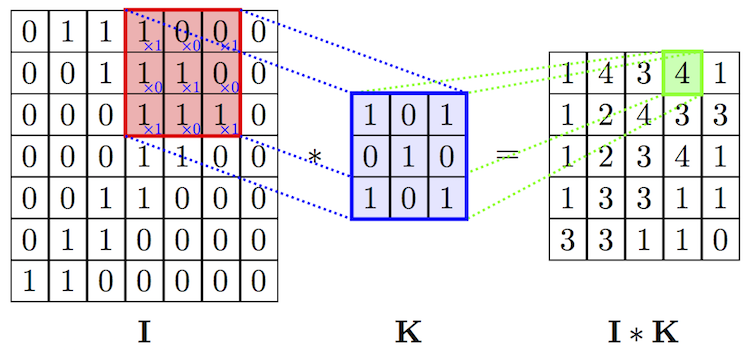
\includegraphics[scale=1.2]{images/convolve.png}
        \caption{Convolution applied to an 8 x 8 image}
        \label{fig:45}
        \end{figure}

        This patch (or \textit{window}) from the image is then slided by $m$ pixels, called stride, and then the filter is reapplied to get another element on the feature map. This process is repeated until all elements on the feature maps are filled. If the value of a specific element is big, it means that specific part of the image has a strong resemblance of the feature represented by the filter.
        \par
        Feature map is technically another image, which means another matrix. However, in this case it also reduces the size of the image while retaining the important information behind it. This operation is technically very similar to convolution operation in image and signal processing. However, in deep learning, instead of us (human) defining every values in the filter matrix, the value of filter matrix will be automatically adjusted (learned) by neural network, thus allowing neural network to find features by itself, hence the name deep convolutional neural network.  
        \par
        This operation is repeated for every convolutional layers. Since Adam-DQN has 3 convolutional layers, this operation will be applied 3 times and resulted in 64 feature maps of size $2 \times 2$. This feature maps will be fed to a  fully connected layer.
        \item \textbf{Fully Connected Layer}
        Fully connected layers are a simple feedforward neural network layers where each node is connected to every single node in the next layer. Fully connected layer utilizes the standard neural network operation, which is a linear combination (or dot product, in vector form) of all inputs and weights. The feature map from convolutional layer is flattened (from a matrix to a vector) and then the dot product of this vector and the weights vector is computed and then fed into the next fully connected layer. Since there are 64 feature maps with size $2 \times 2$, this layer has 256 ($64 \times 2 \times 2$) units/nodes/weights. This process is repeated for the last layer, resulting in a vector with 2-18 elements, depending on the game. Element $i$ in this vector represents the value of $Q^*(s,a_i)$. Which is our predicted $Q$ value for every action.
        \begin{figure}[H]
            \centering
            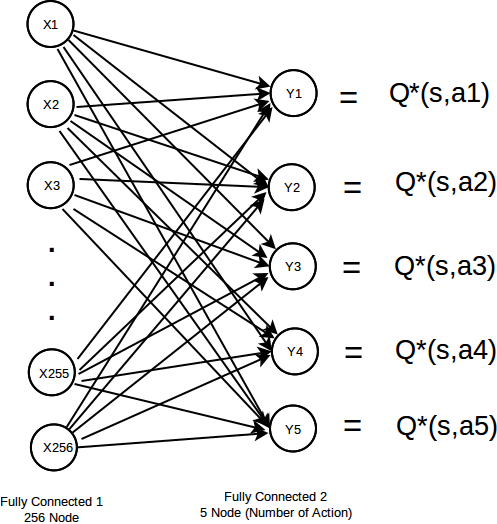
\includegraphics[scale=0.5]{images/FCLayer.png}
            \caption{Illustration of fully connected Layer operations}
            \label{fig:fclayer}
        \end{figure}
        Let the parameters (weights) for every unit in the first fully connected layer equals $\theta_{1 1},\theta_{1 2},\theta_{1 3}, ... , \theta_{256 \ 256} $, Then, the value of node $y_i$ in the next layer:
        \begin{align*}
            b_i&=x_1*\theta_{11}+x_2*\theta_{12}+x_3*\theta_{13}+...+x_{256}*\theta_{1 \ 256} \\
            y_i&=\phi(b_i)
        \end{align*}
        where $\phi()$ represents the activation function (in this case, ReLU). Then,as stated above, $y_i$ represents the value of $Q^*(s,a_i)$. From here, it is trivial to see which actions to take, which is simply $a^*=\argmax_a Q^*(s,a)$. 
        \end{enumerate}
        
        \subsubsection{The Backward Pass - Training}
        As with every other neural network, Deep Q-Network used in Adam-DQL also needs to be trained so that it creates accurate prediction. Adam-DQL uses the \textbf{MSE} (Mean squared error) since Adam-DQL is built to approximate $Q(s,a)$, which means this is a regression task. Similar to Deepmind's Deep Q-Learning, according to equation \ref{eq:36}, for a parameter $\theta_i$, the loss function would be:
        \begin{equation*}
            L(\theta_i)=\E_{s,a,r,s',i \sim D}[(r+\gamma \max_{a'}\hat{Q}(s',a',\theta_i^-)-Q(s,a,\theta_i))^2]
        \end{equation*}
        Where $(R(s,a)+\gamma \max_{a'}\hat{Q}(s',a',\theta_i^-)$ represents the target, and $Q(s,a,\theta_i)$ represents the current prediction. Therefore, given a state (an image of the game) at time $t$, denoted as $s_t$, the training process is as follows:
        \begin{enumerate}
            \item Do a forward pass with the state $s_t$ to the neural network, resulting in a vector $Y_t=[Q(s_t,a_1),Q(s_t,a_2),...]^T$ (see figure \ref{fig:fclayer}) which is the predicted $Q$-function.
            \item From the vector $Y_t$, select the best action $a^*_t$ where $Q(s_t,a^*_t)=\max_a Q(s_t,a)$, and perform that action in the game. The game should now return a new state $s_{t+1}$ as a reaction to $a^*_t$.
            \item Repeat the step 1-2 for $s_{t+1}$ , resulting in a new prediction $Y_{t+1}$ and best action $a^*_{t+1}$.
            \item Observe the reward $r_{t+1}$, and calculate $r_{t+1}+\gamma \max_{a'}\hat{Q}(s',a',\theta_i^-)$ where $\hat{Q}(s',a',\theta_i^-)$ simply means $Q(s_{t+1},a^*_{t+1})=\max_a Q(s_{t+1},a)$ (the maximum value of vector $Y_{t+1}$).
            \item Using the value from $Y_{t+1}$ and step 4, perform a backward pass and compute gradient for all parameters in the network.
        \end{enumerate}
        Using the same example as in figure \ref{fig:fclayer}, the backward pass for all the layers to compute the gradient is as follows:
        \begin{enumerate}
            \item \textbf{Fully Connected Layer} let $y^l_k$ denote the value of a node at layer $l$ and index $k$, from the forward pass:
            \begin{equation*}
                 y^{l+1}_k = \phi (y^l_1)\times \theta_{k1}+\phi (y^l_2) \times \theta_{k2}+\phi (y^l_3)\times \theta_{k3}+...+\phi (y^l_{256})\times \theta_{i256}
            \end{equation*}
            
            The gradient for a parameter $\theta_{ki}$ is then:
            \begin{equation*}
                \frac{\partial L(\theta_i)}{\partial \theta_{ki}}=\frac{\partial L(\theta_i)}{\partial y^{l+1}_k}\frac{\partial y^{l+1}_k}{\partial \theta{ki}}=\frac{\partial L(\theta_i)}{\partial y^{l+1}_k}\phi(y^l_i)
            \end{equation*}
           \item \textbf{Convolutional Layer} let $x^l_{kh}$ denote the value of an element in the layer $l$ and index $k,h$ in the filter.  
           \begin{figure}[H]
               \centering
               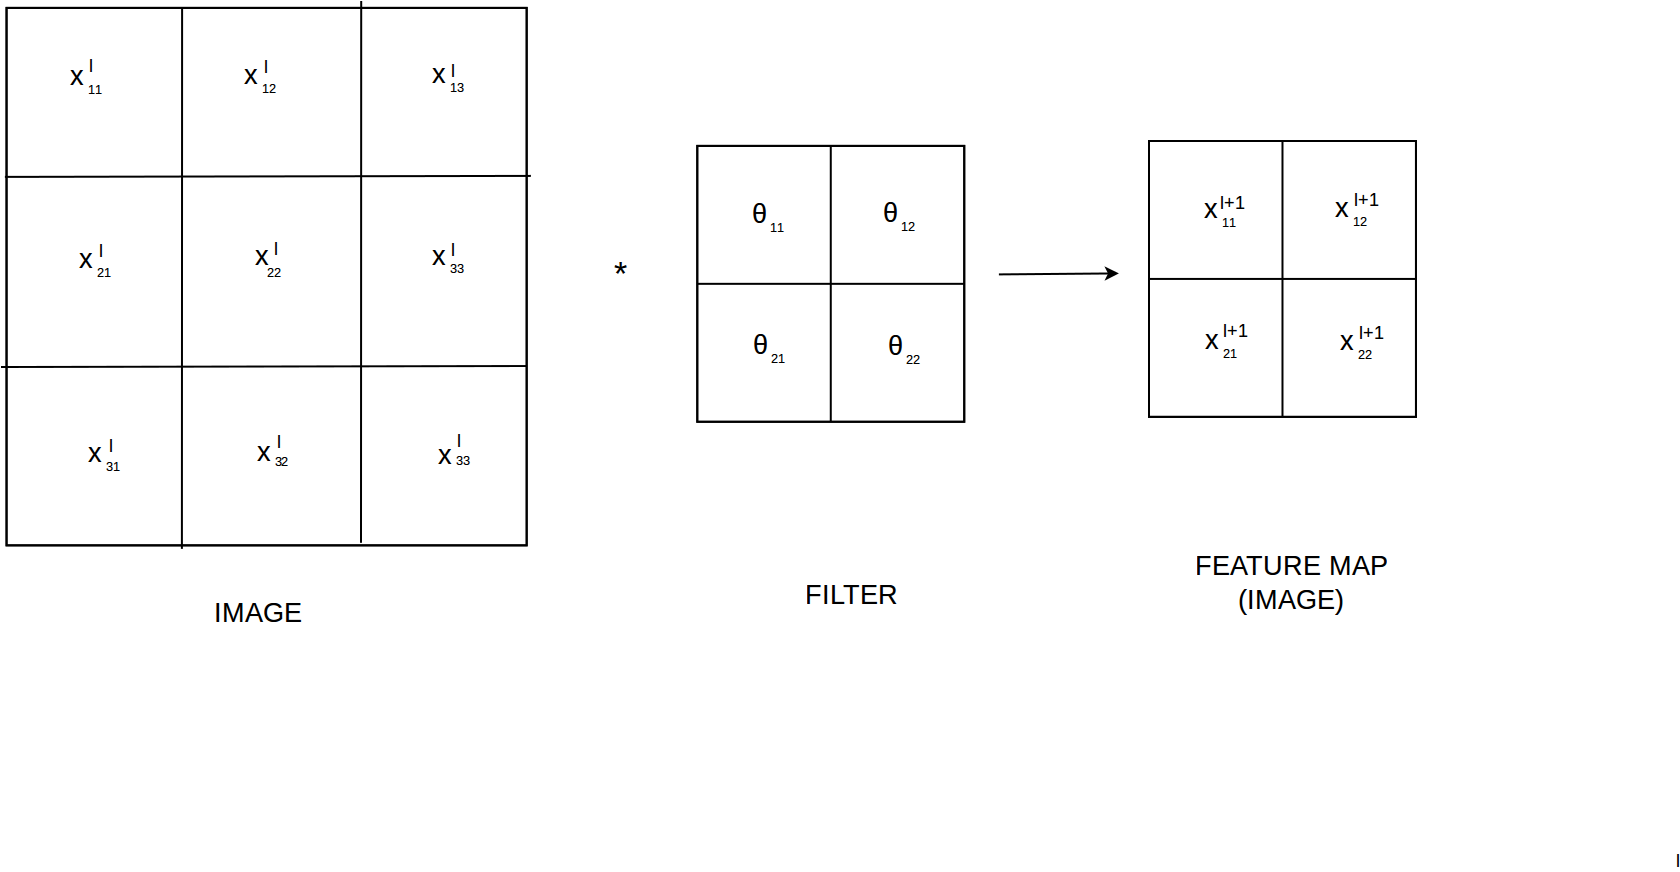
\includegraphics[scale=0.2]{images/convlayer2.png}
               \caption{Visualization of the convolutional layer operations}
               \label{fig:convlayer2}
           \end{figure}From the forward pass:
           \begin{equation*}
               y^{l+1}_{kh} = \phi (y^l_{kh})\times \theta_{11}+\phi (y^l_{k \ h+1}) \theta_{12}+\phi (y^l_{k+1 \ h}) \theta_{21} + \phi (y^l_{k+1 \ h+1}) \theta_{22}
           \end{equation*}
            The gradient for a parameter $\theta_{mn}$ is then:
           \begin{align*}
                \frac{\partial L(\theta_{mn})}{\partial \theta_{mn}}=& \frac{\partial L(\theta_{mn})}{\partial y^{l+1}_{kh}}\phi(y^l_{mn})+\frac{\partial L(\theta_{m \ n+1})}{\partial y^{l+1}_{m\ n+1}}\phi(y^l_{k \ h+1}) \\
                & +\frac{\partial L(\theta_{m+1 \ n})}{\partial y^{l+1}_{m+1\ n}}\phi(y^l_{k+1 \ h})+\frac{\partial L(\theta_{m +1\ n+1})}{\partial y^{l+1}_{m+1\ n+1}}\phi(y^l_{k+1 \ h+1})
            \end{align*}
        \end{enumerate}
    Now that the gradient for all layers can be computed, Adam optimization will be used to update the parameter, refer to section \ref{sec:342} for details.
    
    
    \subsection{Stability and Policy Improvement on Adam-DQN}
    
    As with every reinforcement learning problem, this method suffers from the same exploration-exploitation dilemma, where the agent has to choose whether to use current knowledge and move according to that, or try to explore more hoping that there may be some unexplored state-action combinations that will give us better result.
    \par
    To solve this problem, $\epsilon$-greedy algorithm will be used. As explained in Section \ref{section:26}, the agent will take a random action (exploration) with probability of $\epsilon$ and will take the best action according to current policy with probability $1 - \epsilon$.
    \par
    To further stabilize the Adam-DQN, stabilization technique that is proposed by Deepmind \cite{mnih2015humanlevel} , namely experience replay and target network freezing will be used.
    At each step of the training, dataset $D$ is sampled uniformly at random to get minibatch of experiences of size $M (( s, a, r, s' , i) \sim U (D))$ and perform learning (weights updates) on them.his approach has several advantages over standard online Q-learning. First, each step of experience
    is potentially used in many weight updates, which allows for greater data efficiency.
    Second, learning directly from consecutive samples is inefficient, owing to the strong
    correlations between the samples; randomizing the samples breaks these correlations and therefore reduces the variance of the updates. Third, when learning on-policy the current parameters determine the next data sample that the parameters are trained on. For example, if the maximizing action is to move left then the training samples will be dominated by samples from the left-hand side; if the maximizing action then switches to the right then the training distribution will also switch.
    \par
    It is easy to see how unwanted feedback loops may arise and the parameters could get
    stuck in a poor local minimum, or even diverge catastrophically. By using experience
    replay the behaviour distribution is averaged over many of its previous states,
    smoothing out learning and avoiding oscillations or divergence in the parameters.
    Note that when learning by experience replay, it is necessary to learn off-policy
    (because our current parameters are different to those used to generate the sample), which motivates the choice of Q-learning.
    \par
    The second modification to online $Q$-learning aimed at further improving the
    stability of our method with neural networks is to use a separate network for gen-
    erating the targets y j in the Q-learning update. More precisely, every C updates we
    clone the network $Q$ to obtain a target network $\hat{Q}$ and use $\hat{Q}$
    for generating the $Q$-learning targets y j for the following C updates to Q. This modification makes the
    algorithm more stable compared to standard online Q-learning, where an update
    that increases $Q(s_t ,a_t )$ often also increases $Q(s_{t_+1} ,a)$ for all $a$ and hence also increases
    the target $y_j$ , possibly leading to oscillations or divergence of the policy. Generating
    the targets using an older set of parameters adds a delay between the time an update
    to $Q$ is made and the time the update affects the targets $y_j$ , making divergence or oscillations much more unlikely.
    \par
    All stability improvement techniques explained above are already utilized by Deepmind in \cite{mnih2015humanlevel}. However, this thesis will present a new stability improvement techniques called \textbf{partial training}. On a case where the game $G$ can be broken into sub-problems $G_1, G_2, G_3, ...,G_k$ where $G_1$ represents the easiest sub-problem and $G_k$ represents the hardest sub-problem, our neural network $Q$ is trained for $G_1$ until satisfactory result is achieved. Then the neural network $Q$ is cloned and trained for $G_2$ until it also achieve satisfactory result. This process is repeated until the neural network $Q$ is trained for every sub-problem. Training the neural network on the easier sub-problem $G_1$ allows the neural network to get a lot of rewards (or punishment) allowing the training to proceed. On a case where the game is extremely hard, sometimes an agent might not be able to achieve any form of reward (or punishment), which prevents the actual training to proceed. By kickstarting the neural network on "simplified" version of the problem, our agent should get an idea about what it should do (or not do) on the current game environment faster.
    \par
    Lastly, this thesis will also add technique called \textbf{demonstration}. This technique is firstly utilized on reinforcement learning for robots \cite{DBLP:journals/corr/abs-1709-10089}. This thesis will utilize and use the idea for Adam-DQL to further kickstart the learning process, especially on a game with sparse rewards. On harder games where the rewards are really sparse, it's sometimes not possible for the random exploration (which happens in the early part of training process) to get a reward, thus preventing the neural network to learn and become better at the game. If the agent never gets better, it is very likely that the neural network will ended up diverging from the minima.
    \par
    Fortunately, it is possible to give neural network some initial "knowledge" \cite{DBLP:journals/corr/HesterVPLSPSDOA17} by feeding neural network some example of a proper transition $<s,a,r,s'>$. In layman terms, this means giving some basic state-action condition to built or learn upon. This will be achieved by storing human-created transitions $<s,a,r,s'>$ into the  replay memory $D$. This way, demonstration can be adapted into Adam-DQL as an initial step, without changing the flow of the algorithm itself. This human-created transition will then be replaced by actual replay memory from the agent, if the size replay memory buffer exceed the replay memory capacity.  
    
    \subsection{Preprocessing}
    \label{sec:preprocessing}
        The standard environment for modern games uses at least $256 \times 256$ pixels image for each frame. For modern technology, this is still considered low quality image. However, computing a multiple layers of convolutional neural network for this size is still very costly. Assuming only raw pixels are used, the convolutional part of the neural network needs to be on the same size. Not only convolutional layer that big is expensive both memory and CPU-wise, some part of the screen is mostly unused. Using that unused (unimportant) pixels as an input will only lead to divergence, since they adds more noise to our training data. Therefore, we need to define an preprocessing function $\phi$, that will crop the screen so that only the gameplay part of the screen is used. Preprocessing is a very vital process in Adam-DQL. Not only that it saves memory, it also further simplifies the features that the agent need to learn on the learning process. An image, in this case the game's screen capture, is represented as matrix of pixel values [0-255]. This thesis applies 2 preprocessing techniques, the first one is RGB to grayscale translation. For most games, colors don't actually contribute to how the game should be played, so it's logical to simply remove the colors and transform the image to grayscale. This is really important because it reduces the amount of matrices that will be fed to the neural network. Color image will have a 3 matrices associated with each image, one for each of the colour channels (red, green and blue). While grayscale image is simply a matrix of pixel values.
    \par
    The second one is image resizing, instead of using $256 \times 256$ pixels (the original image size), our processing map will resize the image to $84 \times 84$ pixels. This means our preprocessing map $\phi$ will output an $84 \times 84$ matrix with pixel values of [0-255]. 
    
    \begin{figure}[H]
        \centering
        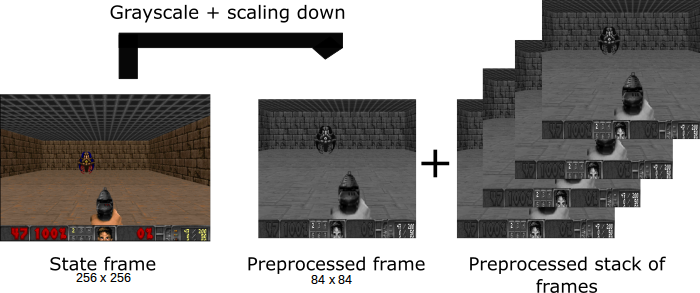
\includegraphics[scale=0.5]{images/preprocessing.png}
        \caption{Game Image Preprocessing}
        \label{fig:44}
    \end{figure}
    
    Also, 2-4 images will be used for every single step and stacked to each other, as 1 image simply cant represent any movement or condition. Which means our final output from this process is  $84 \times 84 \times 4$ (frame)  matrices.
    
    \subsection{Algorithm Review}

            \begin{algorithm}[H]\label{alg:7}
            
            \textbf{Require:} Replay memory $D$ with capacity $N$ \\
            \textbf{Require:} Initial parameter $\theta_0$ \\
            \textbf{Require:} Step size $\epsilon$ \\
            \textbf{Require:} Small constant $\delta $ for numerical stability \\
            \textbf{Require:} Exponential decay rate $\rho_1$ and $\rho_2$ \\
            \ForEach{episode $e$, unless stop condition satisfied}
                {
                
                Get initial state $s_0$ and preprocessed state $\phi_0$ \\
                Initialize 1st and 2nd moment variables $s=0, r=0$ \\
                Store demonstration data in replay memory $D$ \\
               \ForEach{timestep $t$ in current episode $e$}
                    {
                       Using $\epsilon$-greedy policy, select action $a_t$\\
                       Execute action $a_t$\\
                       Observe following state $s_{t+1}$ and and whether it is terminal ($i_{t+1}$)\\
                       Preprocess the state $\phi_{t+1}=\phi(s_{t+1})$ \\
                       Store transition $(\phi_{t},r_t,a_t,\phi_{t+1},i_{t+1})$\\
                       Sample random minibatch of transitions $(\phi_j,r_j,a_j,\phi_{j+1},i_{j+1})$   of size $M$ from $D$\\
                       \ForEach{sample in the minibatch}
                            {
                                \eIf{$i_j+1$ is true}{$y_j=r_j$}
                                {$y_j=r_j+\gamma \max_{a'}Q(\phi_{j+1},a',\theta)$}
                            }
                    }
                    Sample a minibatch of $m$ examples from the training set {$x^{(i)},...x^{(m)}$} and corresponding targets $y^{(i)}$ \\
                    Compute gradient estimate: $g \gets \frac{1}{m} \nabla_\theta \sum_i L(f(x^{(i)};\theta_e),y^{(i)}) $ \\
                    Update biased first and second moment estimate: $s,r \gets \rho_{1,2} (s,r)+ (1-\rho_{1,2})g$\\
                    Correct bias in first and second moment: $\hat{s},\hat{r} \gets \frac{s,r}{1-\rho_{1,2}^t}$\\
                    Compute update: $\Delta \theta_e \gets -\frac{\epsilon}{\delta+\sqrt{r}}\bigodot g.$ (Division and square root applied element-wise) \\
                    Apply update: $\theta_e \gets \theta_e +\Delta \theta_e$\\
                    
                }
                

            \caption{Adam-DQN with experience replay and demonstration}
            \end{algorithm}
    \section{Architecture}
    In order to show and experiment with the newly developed Adam-DQL, it is needed to create a software that allows experiment and testing on the new algorithm. Adam-DQL is specifically created to play more complex video-games, hence testing it by letting Adam-DQL agent to play video-games is a must. However, without a properly developed software, Adam-DQL is just program without any meaningful uses. Below is the details of the software developed for this thesis.
    \subsection{General Software Architecture}
    
    The software used in this thesis is shown on figure \ref{fig:41} and consists of 2 main components listed below. The reasoning behind this architechture is based on the analysis done in the next chapter. 
        \subsubsection{Games}
        This is the component that actually runs the game. Most of the time, the actual game source code is not available, Which means there's a need of some \textit{automated extraction} from the game, by utilizing modern desktop-PC features such as screenshot and screen capture, combined with the ability of the agent to simulate a key press on the keyboard. In the case where the game is open source, it's then possible to allow direct interactions between our agent and the game by simply modifying the game's source code. This thesis will provide an example for both cases, allowing the development of an AI that's as general as possible.
    
        \subsubsection{Deep Learning Agent}
        
        This is the \textit{brain} of the software framework. Coming from the fact that the code for all the game isn't available, and that the only accessible data is the pixels. It is needed to create a component to facilitate that so that our deep-learning agent (AI) will be able to interact with the game. This component will retrieve the pixel information from the game, \textit{preprocess} it, and send it to our actual agent in the program, as a preprocessed state ($\phi$).The agent can then process the data and  Whenever the agent decided to do something, the agent will send a signal to this component, that will simulate a button press, since this is the only input method acceptable by the game (unless source code of the game is available). Deep Learning agent will receive the input preprocessed by our framework, and use it as an input for Adam-DQL algorithm. After going through the neural network, Adam-DQL algorithm will send an output (as a signal) to the framework, then to the game. This process can happen in on the learning process (although the output might not be optimal yet) and the playing process (with optimal policy).
    
    \begin{figure}[H]
        \centering
        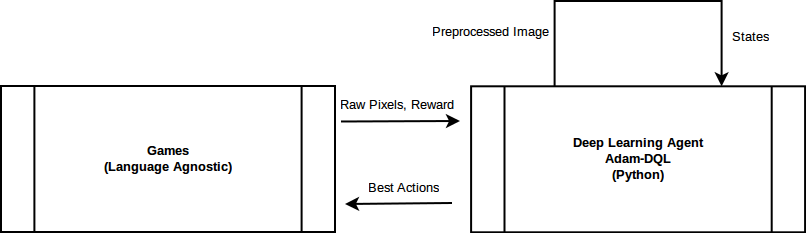
\includegraphics[scale=0.4]{images/framework2block.png}
        \caption{General software architecture}
        \label{fig:41}
    \end{figure}
    
    \subsection{State Representation}
        Despite the algorithm being applicable to a raw pixels as an input, simply putting all the raw pixels into the neural network is never a good idea. Technically, raw pixels contains all the information, that sometimes shouldn't be available for the players, for example: an agent shouldn't know that there's enemy 3 frames after the current frame. That's why Adam-DQN has a CNN (Convolutional neural network) to classify value of the pixels and change that into useful information. This information is then called \textit{classified data}, that will be selectively given to the agent for training. 
        \noindent
        This state representation for Adam-DQN is presented in figure \ref{fig:42}
        \begin{figure}[H]
            \centering
            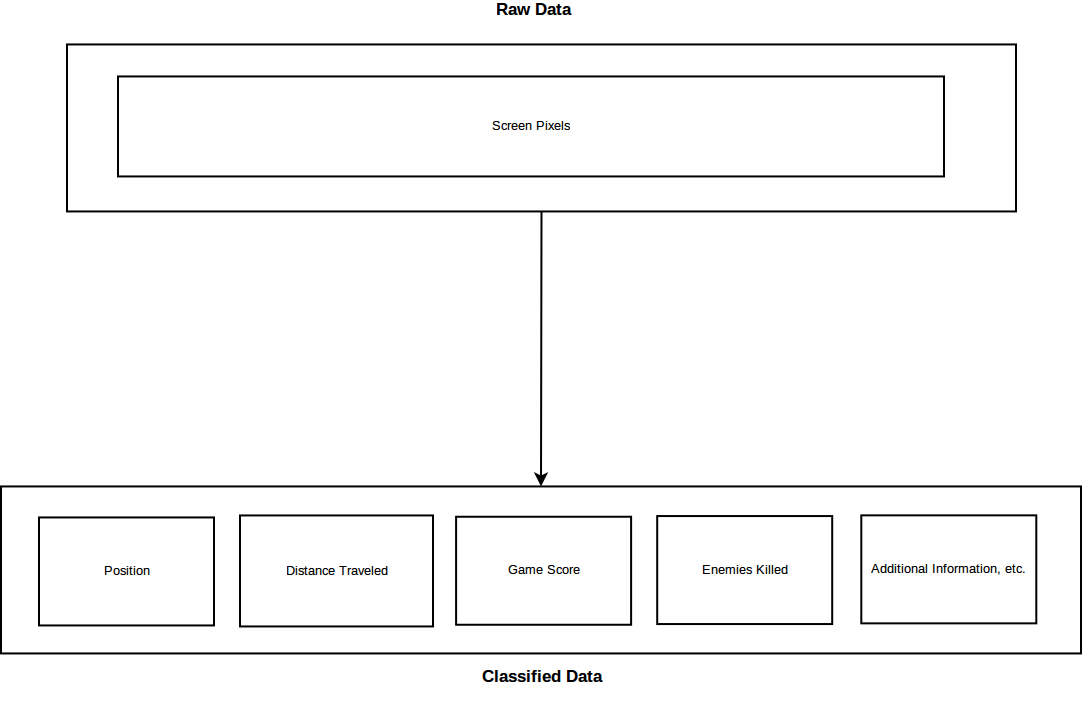
\includegraphics[scale=0.35]{images/data.png}
            \caption{State Representation Sample}
            \label{fig:42}
        \end{figure}
    
    
    \subsection{Neural Network Structure}
    The exact architecture of our neural network, shown schematically in figure 4.3, is as follows. The input to the neural network consists of an $84 \times 84 \times 4$ image produced by the preprocessing map $\phi$. The first hidden layer convolves 16 filters of $8\times 8$ with stride 4 with the input image and applies a rectifier nonlinearity. The second hidden layer convolves 32 filters of $4 \times 4$ with stride 2, again followed by a rectifier nonlinearity. This is followed by a third convolutional layer that convolves 64 filters of $2 \times 2$ with stride 1 followed by a rectifier. The final hidden layer is fully-connected and consists of 256 rectifier units. The output layer is a fully-connected linear layer with a single output for each valid action. The number of valid actions are generally around 2-18, depending on the game.
    
    \begin{figure}[H]
        \centering
        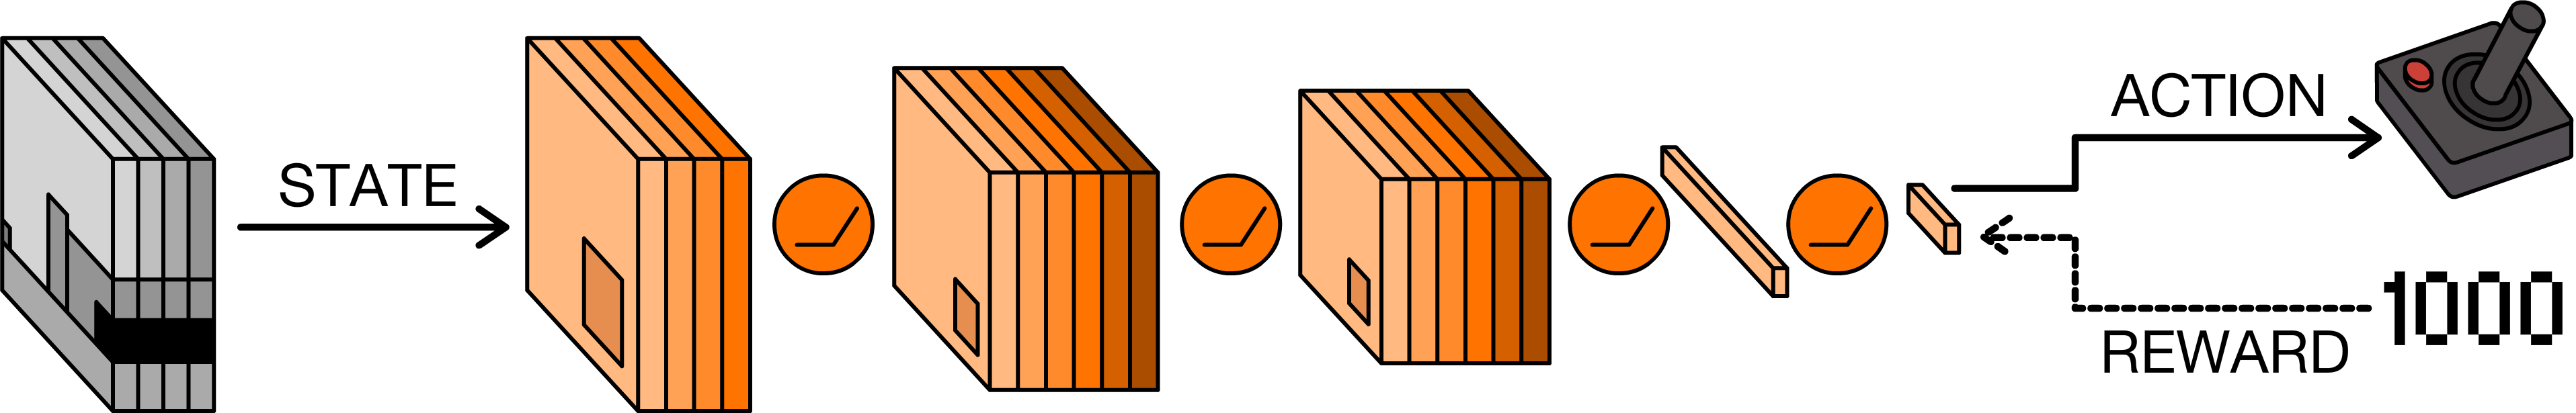
\includegraphics[scale=0.1]{images/dqn.png}
        \caption{Architecture of Adam-DQN}
        \label{fig:43}
    \end{figure}
    
    \iffalse
    \section{Implementation and Agent's Flow}
    In section \ref{sec:4}, Adam-DQL algorithm and its policy improvement strategy are explained. However, one might need additional explanation regarding how this algorithm should be implemented (programmatically). Therefore, this section is dedicated to explain the low level (program level) implementation of Adam-DQL algorithm. Adam-DQL requires states (pixels) and rewards to properly decide which action is optimal for a specific state. Thus, the process of getting an image until the decision of which actions to make will be explained in the following section.
    
    \subsection{Preprocessing}
    
    As stated in Section \ref{sec:preprocessing}, preprocessing is a very vital process in Adam-DQL. Not only that it saves memory, it also further simplifies the features that the agent need to learn on the learning process. An image, in this case the game's screen capture, is represented as matrix of pixel values [0-255]. This thesis applies 2 preprocessing techniques, the first one is RGB to grayscale translation. For most games, colors don't actually contribute to how the game should be played, so it's logical to simply remove the colors and transform the image to grayscale. This is really important because it reduces the amount of matrices that will be fed to the neural network. Color image will have a 3 matrices associated with each image, one for each of the colour channels (red, green and blue). While grayscale image is simply a matrix of pixel values.
    \par
    The second one is image resizing, instead of using $256 \times 256$ pixels (the original image size), our processing map will resize the image to $84 \times 84$ pixels. This means our preprocessing map $\phi$ will output an $84 \times 84$ matrix with pixel values of [0-255]. 
    
    \begin{figure}[H]
        \centering
        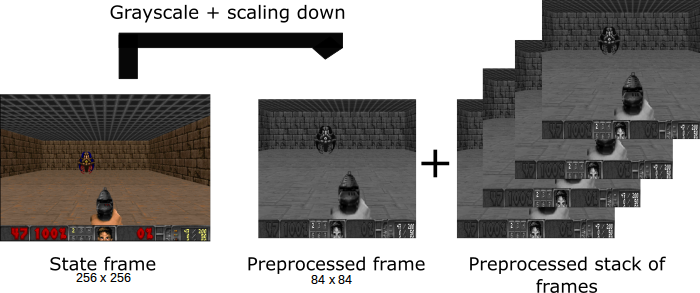
\includegraphics[scale=0.5]{images/preprocessing.png}
        \caption{Game Image Preprocessing}
        \label{fig:44}
    \end{figure}
    
    Also, as explained before, 4 images will be used for every single step and stacked to each other, as 1 image simply cant represent any movement or condition. Which means our final output from this process is  $84 \times 84 \times 4$ (frame)  matrices.
        
    \subsection{Deep Learning}
    Chapter \ref{sec:dql} already explained the need of deep neural networks to approximate the value of $Q(s,a)$. Adam-DQL uses DQN (Deep Q-Network), a deep convolutional neural network proposed by Deepmind to approximate the value of $Q(s,a)$. This section will discuss the computational process inside each operation in Deep Q-Network, which mainly consist of two parts, the forward pass (predicting the value of $Q(s,a)$) and the backward pass (training).
    \subsubsection{The Forward Pass - Prediction}
    The forward pass is the process of feeding the image from our game to our neural network, and receive the predicted $Q(s,a)$ values as an output. Deep Q-Network consists of 3 convolutional layers and 2 fully connected layers. 
    \begin{enumerate}
        \item \textbf{Convolutional Layers}
        This layer is what defined a convolutional neural networks. Convolutional layer \textit{interwine} two sources of information. Practically, convolutional layer builds a feature map that shows the likeability of a feature appearing in the image. This is achieved by applying a so called \textit{filter} or \textit{kernel} to an image. Filter is a matrix of weights analogous to a vector of weights in a standard feedforward neural network. The real values of the filter matrix change with each learning iteration over the training set, indicating that the network is learning to identify which regions are of significance for extracting features from the data. When applied to an image, denoted by operator $*$, small parts of the image matrix are taken (with the same size as the filter), and dot product of the image and the kernel is calculated. This will be the value of each entry in the feature maps. Below is an example of 1 filter applied to an $8 \times 8$ image matrix. 
        \begin{figure}[H]
        \centering
        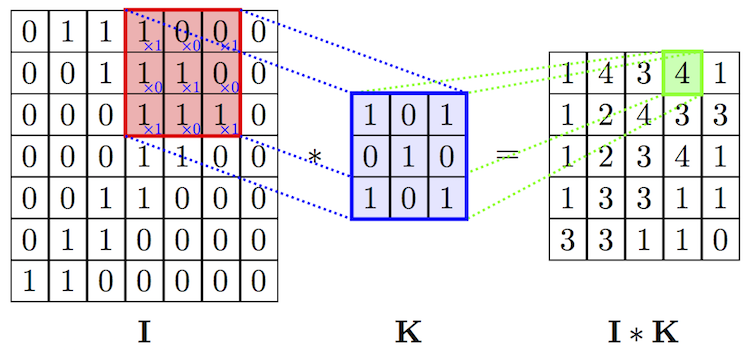
\includegraphics[scale=1.2]{images/convolve.png}
        \caption{Convolution applied to an 8 x 8 image}
        \label{fig:45}
        \end{figure}
        

        This patch (or \textit{window}) from the image is then slided by $m$ pixels, called stride, and then the filter is reapplied to get another element on the feature map. This process is repeated until all elements on the feature maps are filled. If the value of a specific element is big, it means that specific part of the image has a strong resemblance of the feature represented by the filter.
        \par
        Feature map is technically another image, which means another matrix. However, in this case it also reduces the size of the image while retaining the important information behind it. This operation is technically very similar to convolution operation in image and signal processing. However, in deep learning, instead of us (human) defining every values in the filter matrix, the value of filter matrix will be automatically adjusted (learned) by neural network, thus allowing neural network to find features by itself, hence the name deep convolutional neural network.  
        \par
        This operation is repeated for every convolutional layers. Since Adam-DQN has 3 convolutional layers, this operation will be applied 3 times and resulted in 64 feature maps of size $2 \times 2$. This feature maps will be fed to a  fully connected layer.
        \item \textbf{Fully Connected Layer}
        Fully connected layers are a simple feedforward neural network layers where each node is connected to every single node in the next layer. Fully connected layer utilizes the standard neural network operation, which is a linear combination (or dot product, in vector form) of all inputs and weights. The feature map from convolutional layer is flattened (from a matrix to a vector) and then the dot product of this vector and the weights vector is computed and then fed into the next fully connected layer. Since there are 64 feature maps with size $2 \times 2$, this layer has 256 ($64 \times 2 \times 2$) units/nodes/weights. This process is repeated for the last layer, resulting in a vector with 2-18 elements, depending on the game. Element $i$ in this vector represents the value of $Q^*(s,a_i)$. Which is our predicted $Q$ value for every action.
        \begin{figure}[H]
            \centering
            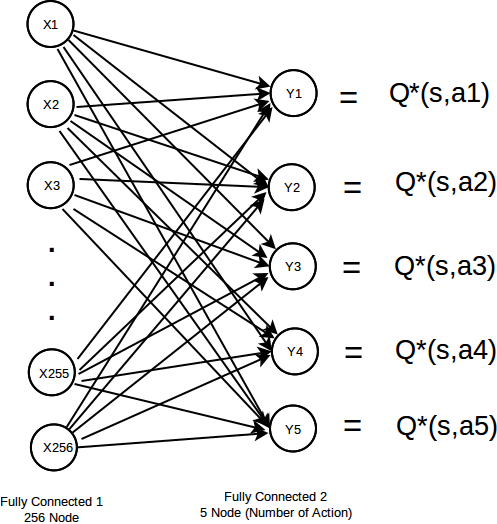
\includegraphics[scale=0.5]{images/FCLayer.png}
            \caption{Illustration of fully connected Layer calculations}
            \label{fig:fclayer}
        \end{figure}
        Let the parameters (weights) for every unit in the first fully connected layer equals $\theta_{1 1},\theta_{1 2},\theta_{1 3}, ... , \theta_{256 \ 256} $, Then, the value of node $y_i$ in the next layer:
        \begin{align*}
            b_i&=x_1*\theta_{11}+x_2*\theta_{12}+x_3*\theta_{13}+...+x_{256}*\theta_{1 \ 256} \\
            y_i&=\phi(b_i)
        \end{align*}
        where $\phi()$ represents the activation function (in this case, ReLU). Then,as stated above, $y_i$ represents the value of $Q^*(s,a_i)$. From here, it is trivial to see which actions to take, which is simply $a^*=\argmax_a Q^*(s,a)$. 
        \end{enumerate}
        
        \subsubsection{The Backward Pass - Training}
        As with every other neural network, Deep Q-Network used in Adam-DQL also needs to be trained so that it creates accurate prediction. Adam-DQL uses the \textbf{MSE} (Mean squared error) since Adam-DQL is built to approximate $Q(s,a)$, which means this is a regression task. Similar to Deepmind's Deep Q-Learning, according to Equation \ref{eq:36}, for a parameter $\theta_i$, the loss function would be:
        \begin{equation*}
            L(\theta_i)=\E_{s,a,r,s',i \sim D}[(r+\gamma \max_{a'}\hat{Q}(s',a',\theta_i^-)-Q(s,a,\theta_i))^2]
        \end{equation*}
        Where $(R(s,a)+\gamma \max_{a'}\hat{Q}(s',a',\theta_i^-)$ represents the target, and $Q(s,a,\theta_i)$ represents the current prediction. Therefore, given a state (an image of the game) at time $t$, denoted as $s_t$, the training process is as follows:
        \begin{enumerate}
            \item Do a forward pass with the state $s_t$ to the neural network, resulting in a vector $Y_t=[Q(s_t,a_1),Q(s_t,a_2),...]^T$ (see Figure \ref{fig:fclayer}) which is the predicted $Q$-function.
            \item From the vector $Y_t$, select the best action $a^*_t$ where $Q(s_t,a^*_t)=\max_a Q(s_t,a)$, and perform that action in the game. The game should now return a new state $s_{t+1}$ as a reaction to $a^*_t$.
            \item Repeat the step 1-2 for $s_{t+1}$ , resulting in a new prediction $Y_{t+1}$ and best action $a^*_{t+1}$.
            \item Observe the reward $r_{t+1}$, and calculate $r_{t+1}+\gamma \max_{a'}\hat{Q}(s',a',\theta_i^-)$ where $\hat{Q}(s',a',\theta_i^-)$ simply means $Q(s_{t+1},a^*_{t+1})=\max_a Q(s_{t+1},a)$ (the maximum value of vector $Y_{t+1}$).
            \item Using the value from $Y_{t+1}$ and step 4, perform a backward pass and compute gradient for all parameters in the network.
        \end{enumerate}
        Using the same example as in Figure \ref{fig:fclayer}, the backward pass for all the layers to compute the gradient is as follows:
        \begin{enumerate}
            \item \textbf{Fully Connected Layer} let $y^l_k$ denote the value of a node at layer $l$ and index $k$, from the forward pass:
            \begin{equation*}
                 y^{l+1}_k = \phi (y^l_1)\times \theta_{k1}+\phi (y^l_2) \times \theta_{k2}+\phi (y^l_3)\times \theta_{k3}+...+\phi (y^l_{256})\times \theta_{i256}
            \end{equation*}
            
            The gradient for a parameter $\theta_{ki}$ is then:
            \begin{equation*}
                \frac{\partial L(\theta_i)}{\partial \theta_{ki}}=\frac{\partial L(\theta_i)}{\partial y^{l+1}_k}\frac{\partial y^{l+1}_k}{\partial \theta{ki}}=\frac{\partial L(\theta_i)}{\partial y^{l+1}_k}\phi(y^l_i)
            \end{equation*}
           \item \textbf{Convolutional Layer} let $x^l_{kh}$ denote the value of an element in the layer $l$ and index $k,h$ in the filter.  
           \begin{figure}[H]
               \centering
               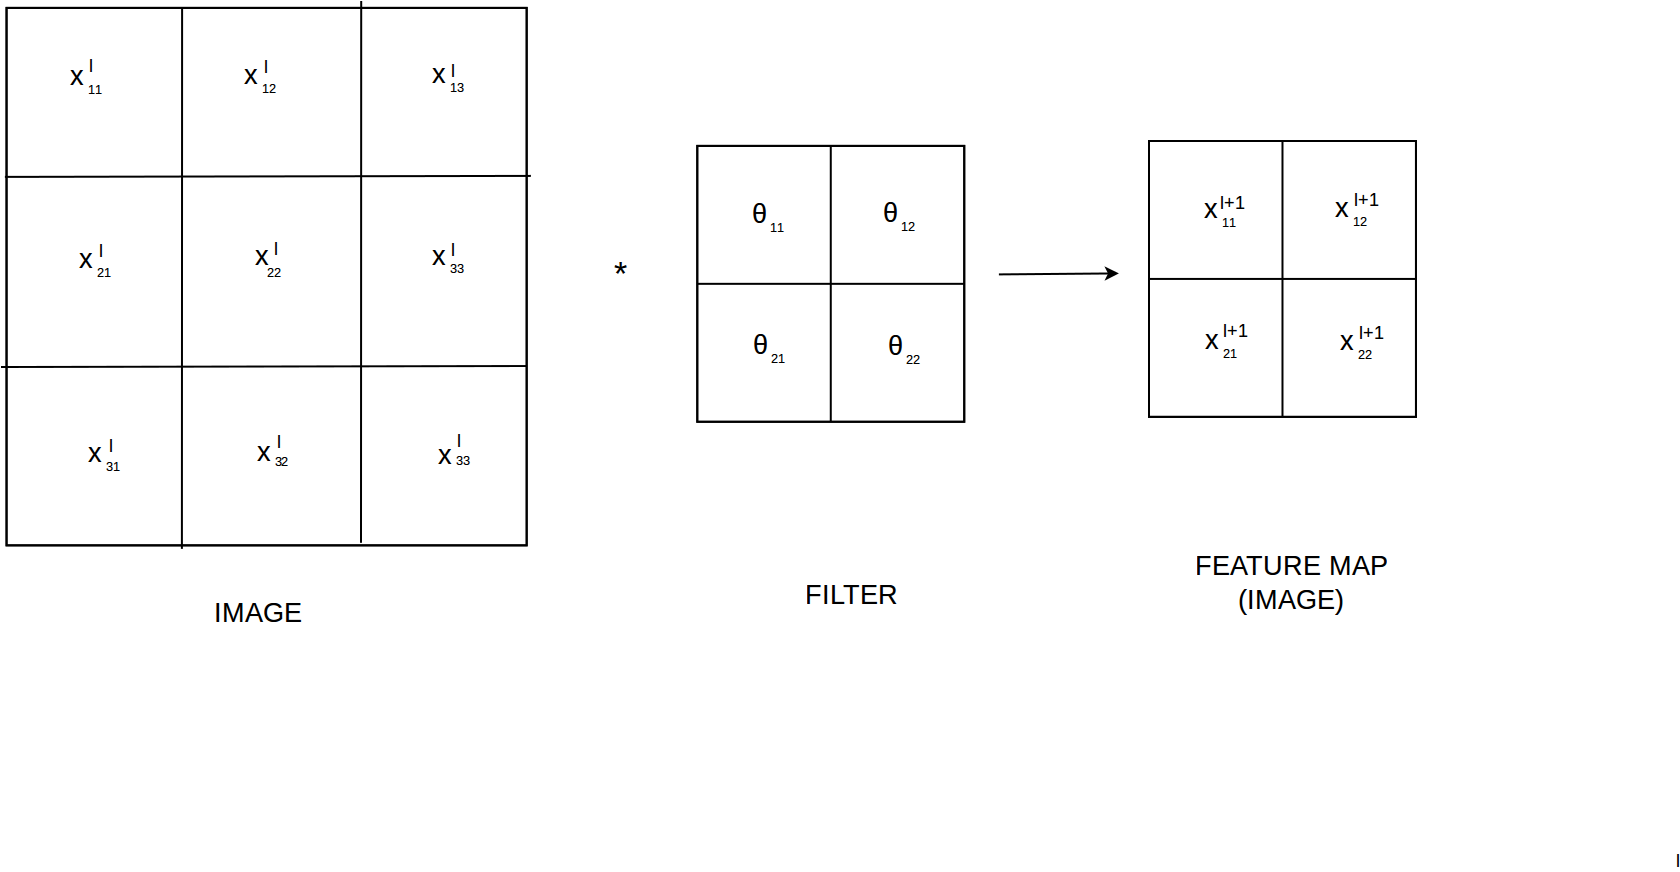
\includegraphics[scale=0.2]{images/convlayer2.png}
               \caption{Visualization of the convolutional layer operations}
               \label{fig:convlayer2}
           \end{figure}From the forward pass:
           \begin{equation*}
               y^{l+1}_{kh} = \phi (y^l_{kh})\times \theta{11}+\phi (y^l_{k \ h+1}) \theta{12}+\phi (y^l_{k+1 \ h}) \theta{21} + \phi (y^l_{k+1 \ h+1}) \theta{22}
           \end{equation*}
            The gradient for a parameter $\theta_{mn}$ is then:
           \begin{align*}
                \frac{\partial L(\theta_{mn})}{\partial \theta_{mn}}=& \frac{\partial L(\theta_{mn})}{\partial y^{l+1}_{kh}}\phi(y^l_{mn})+\frac{\partial L(\theta_{m \ n+1})}{\partial y^{l+1}_{m\ n+1}}\phi(y^l_{k \ h+1}) \\
                & +\frac{\partial L(\theta_{m+1 \ n})}{\partial y^{l+1}_{m+1\ n}}\phi(y^l_{k+1 \ h})+\frac{\partial L(\theta_{m +1\ n+1})}{\partial y^{l+1}_{m+1\ n+1}}\phi(y^l_{k+1 \ h+1})
            \end{align*}
        \end{enumerate}
    Now that the gradient for all layers can be computed, Adam optimization will be used to update the parameter, refer to Section \ref{sec:342} for details.
    \fi

%=================================CHAPTER V=========================================

\chapter{EXPERIMENT AND RESULTS}
\thispagestyle{fancy}

    Based on the presented concepts thus far, our presented Adam-DQL algorithm relies on applying a faster gradient optimization technique to an already established Deep Q-Learning techniques made by Deepmind. Despite the wide range of possible applications (especially in modern games), as a proof of concept, this thesis narrowed down to a handful of illustrative environments that represents varied elements in modern video games. Adam-DQL agent is deployed, then tested on these environments, followed by a thorough analysis and insights about how the agent is performing on these environments.
    
    \section{Experimental Setup}
    In all experiments, the following definitions are used:
    \begin{itemize}
        \item \textit{Timesteps} is a unit used to indicate the simulation or game time. For every timestep, images/frames are fed into the neural network. This term can be used interchangeably with \textit{frames}.
        \item \textit{Episode} is an entire play of the game from the start until the game over signal, or often referred as terminal state. 1 episode could last for few hundred frames.
        \item \textit{Raw pixels} is the unprocessed raw values from a screen capture of a game.
        \item \textit{State} is a preprocessed image from the game, that is ready to be fed into the neural network. 
        \item \textit{Local Minima} indicates a point where the value of the error or loss function is smaller than all the neighboring points
        \item \textit{Global Minima} indicates a point where the value of the error or loss function is the smallest across all points.
        \item \textit{Regression} (programming terms) is a condition where a program becomes worse throughout updates.
        \item \textit{Annealing} means linearly reducing the value of a variable.
        \item \textit{Oscillates} is a condition where an AI agent stays on the same level of performance because of regression-improvement loop.
        \item \textit{Policy} indicates a function $\pi: S \to A$ that maps state into an action. 
    \end{itemize}
    
    In all experiments, the following setup was used:
    \begin{itemize}
        \item All of the environments used in this thesis are made on Python 2.7.3. All GUI elements are drawn on top of PyGame and Python-tk toolkit.
        \item Adam-DQL agent are built on top of Google's deep learning library, Tensorflow. Specifically, Tensorflow 1.7.0b.
        \item Adam-DQL agent are implemented as a Python class/module for future reuse and research purposes.
        \item Adam-DQL is trained using GPU-CUDA with the following specifications:
        \begin{table}[H]
            \centering
            
            \label{specs}
            \begin{tabular}{|l|l|l|}
            \hline
            \textbf{Server Name}     & \textbf{Desktop}    & \textbf{Laptop}     \\ \hline
            \textbf{OS}              & Ubuntu 18.04        & Ubuntu 16.04        \\ \cline{1-1}
            \textbf{Num. CPU's}      & 4                   & 8                   \\ \cline{1-1}
            \textbf{CPU Clock Freq.} & 3.1 GHz             & 2.8 GHz             \\ \cline{1-1}
            \textbf{Num. CPU Cores}  & 4                   & 8                   \\ \cline{1-1}
            \textbf{Ram Size}        & 8 GB                & 16GB                \\ \cline{1-1}
            \textbf{GPU 1 Type}      & Geforce GTX 750 Ti & Geforce GTX 1050 Ti \\ \cline{1-1}
            \textbf{GPU 1 mem. size} & 2 GB                & 4 GB                \\ \hline
            \end{tabular}
            \caption{Hardware Specifications}
        \end{table}
        \item The result points are taken every 10000 training episodes, unless stated otherwise (for comparison purposes).
        \item The training process ends at 500000 episodes unless the neural network doesn't grow any further before 500000 episodes.
        \item The value of the reward at every point is the average reward from 100 games played by the agent at that checkpoint.
        \item Since this is a reinforcement learning problem, the same datasets are used for training and validation.
    \end{itemize}
    \section{Architecture Analysis}
    
    Before Adam-DQL agent can be tested on our proposed environments, The software framework architecture needs to be finalized first. The chosen architecture is already shown in Chapter \ref{sec:4}, nevertheless, the reasoning behind that decision is still unclear. This section will go in depth on all the possible architecture and justify the decision on the last chapter. There's 3 possible software architecture for Adam-DQL, namely 1-block, 2-blocks and 3-blocks system.
    
    \subsection{1-block architecture}
         The 1-block architecture, as the name suggests, consist of only one software block. This means that the testing environment (the game) and the agent is merged into one program. The game will be modified heavily, and the agent will be integrated inside the game's code. This is the ideal scenario for practical usage of the AI, as this is the architecture that a normal game with AI will use in real life. However, this architecture is not suitable for testing and educational purposes, as the agent's code is made to work only with this specific environment. Changing environment (testing other game) means creating a new software from scratch. In layman terms, this architecture is the least general of all 3, while also being the cleanest and the fastest, because there's no inter-program communication involved.
         
        \begin{figure}[H]
            \centering
            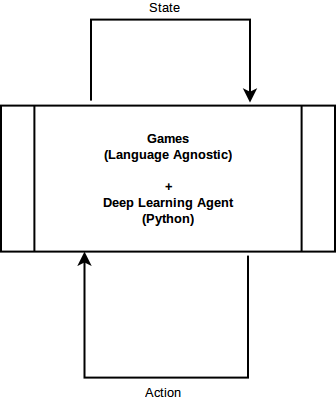
\includegraphics[scale=0.5]{images/framework1block.png}
            \caption{The 1-block architecture}
            \label{fig:1block}
        \end{figure}
 
    \subsection{2-blocks architecture}
        The 2-blocks architecture, consist of 2 software blocks, the environment (the game) and the agent. This means that the testing environment is separated from the agent, and only modified slightly to accommodate the requirements of the agent. The environment will send the raw pixels (image) to the agent, and agent will perform the preprocessing step, resulting in the actual state required by Adam-DQL algorithm. The agent will then perform Adam-DQL algorithm and send the best action back to the environment, and the environment will perform that action. This architecture will work generally for most games. However, some games are built like a "blackbox", and these modifications might not be possible. This architecture utilizes few inter-program communication, which might be a bit challenging to build. As this architecture seems to provide the balance between generality, ease of development and speed, this architecture is then \textbf{chosen for this thesis}.
        
           \begin{figure}[H]
            \centering
            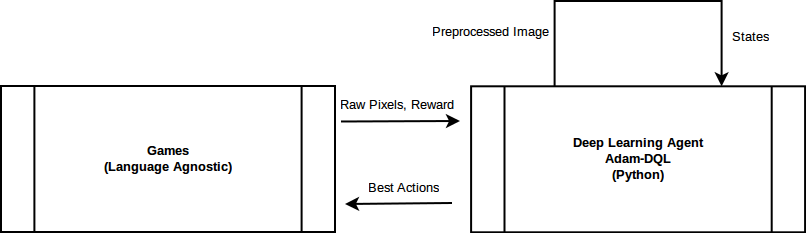
\includegraphics[scale=0.4]{images/framework2block.png}
            \caption{The 2-block architecture}
            \label{fig:2block}
        \end{figure}
 
    \subsection{3-blocks architecture}
        The 3-blocks architecture is the most complex architecture that Adam-DQL can use. This architecture utilizes some kind of middleware, the third program that translates the raw data from the game into the usable data (state) for the agent. The game only sends the memory buffer, and the middleware will read the memory buffer and translates it into preprocessed image (state) and reward. This data will be processed by the agent, to receive the best action for that state. Instead of sending the action directly into the game, this action will be sent into the middleware, and the middleware will simulate a keyboard/input that corresponds to that action. This way, there's almost no modification needed for the environment, thus resulting in the most general architecture. However, this architecture is the least trivial to implement, requiring low-level (memory level) knowledge for every game, and also the slowest. This architecture is what deepmind used in their publications, resulting in them being able to test on a huge set of games \cite{mnih2015humanlevel}.
           \begin{figure}[H]
            \centering
            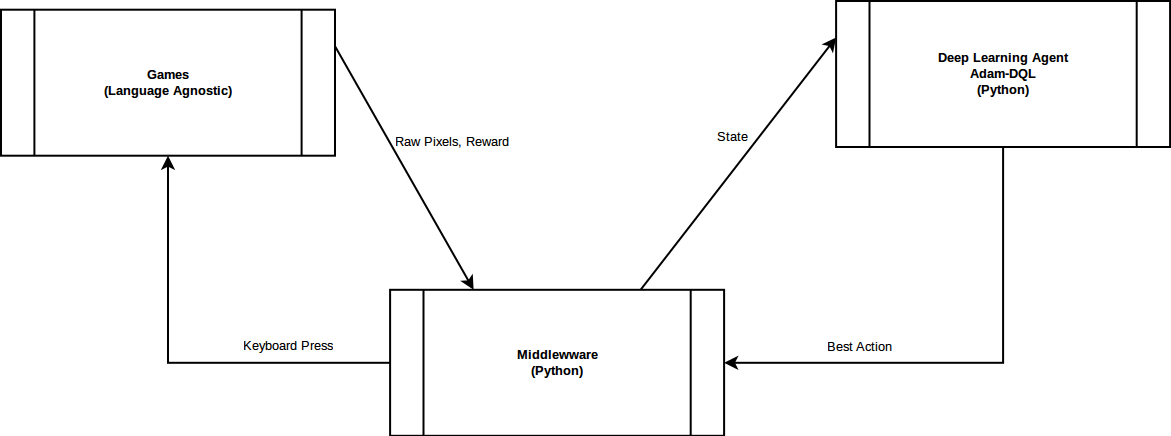
\includegraphics[scale=0.33]{images/framework3block.png}
            \caption{The 3-block architecture}
            \label{fig:3block}
        \end{figure}
        
    
 
        
  \section{Proposed Environments} \label{environment}
	
	Below are some game environments that will be used to test the learning capability of Adam-DQL. These game environments are specifically chosen to showcase Adam-DQL's ability to learn different type of games. The purpose of each chosen environment will be explained on the second part of this chapter. As explained in Section \ref{sec:4}, These information aren't given to the Adam-DQL agents instead are meant to give readers an idea about the testing environment (difficulties and types). The agents itself only receive raw pixels (as states) and rewards. 
	\subsection{Cartpole/Inverted Pendulum}
    	   
    Consider tasks in which an agent interacts with an environment,
    in this case a simplified inverted pendulum problem without friction, often referred as cartpole \cite{bartosutton}.  A pole is attached by an un-actuated joint to a cart, which moves along a frictionless track. Our main goal is to balance the pole by utilizing an applied force to both left and right ends of the cart.
    
    \begin{figure}[H]
        \centering
        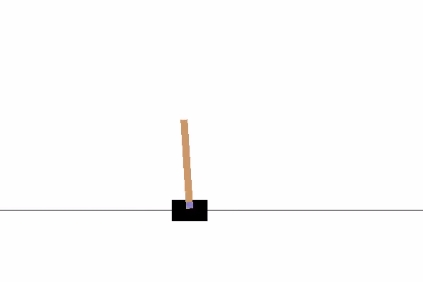
\includegraphics[scale=0.5]{images/cartpole.png}
        \caption{Image of the OpenAI Gym's Cartpole problem}
        \label{fig:51}
    \end{figure}
    
    The problem dynamics has the following equation, with $x$ being the horizontal position of the cart, and $\theta$ being the angle of the pole and the vertical axis:
    
        \begin{gather*}
                 x_{t+1}=x_t+\tau \dot{x_t}\\
            \dot{x}_{t+1}=\dot{x_t}+\tau \ddot{x_{t}}\\
            \ddot{x_t}=\frac{F+ml(\dot{\theta_t^2} sin(\theta_t) - \ddot{\theta_t}cos(\theta_t)}{m+M}\\
             \theta_{t+1}=\theta_t+\tau \dot{\theta_t}\\
            \dot{\theta}_{t+1}=\dot{\theta_t}+\tau \ddot{\theta_{t}}\\
            \ddot{\theta_t}=\frac{g sin(\theta_t) - cos(\theta_t)\frac{-F-\dot{\theta_t^2}sin(\theta_t) }{m+M}}{l(\frac{4}{3}-\frac{m cos(\theta_t)^2}{m+M})}\\
        \end{gather*}
       
       where $\tau = 0.02$(seconds/step), the length of the pole $l = 0.5(m)$, $F = \pm10$ is the magnitude of the force applied by our agent. The mass of the pole is $m = 0.1(kg)$, mass of the cart $m = 1.0(kg)$ and gravity $g = 9.8(ms^{−2} )$. It's important to note that equations above aren't differential equations, rather, a simplified algebraic equations representing the same problem.
       \begin{itemize}
        \item \textbf{Environment dynamics $s_t$} : $(x_t,\dot{x}_t,\theta_t,\dot{\theta}_t) \in S$, consisting of a state for the agent, following the dynamics presented above. The starting position is $s_0$ , a uniform randomized 4-D vector with boundaries for each variable of $[-0.05,0.05]$. The goal is to balance the pole for 195 timesteps in average. Mathematically balancing the pole means, keeping $||x_t|| \leq 2.4(m)$ or $||\theta_t||\leq\frac{24}{360}(rad)$.
        \item \textbf{A finite (2) set of actions A}, Apply force to the left $(a=-1 : F=-10(N))$ or apply force to the right $(a=1 : F=10(N))$.
        \item \textbf{A reward function} $r=R(s_t,a_t,s_{t+1})$, which is $r=1$ for every timestep in which the agent managed to prevent the game from ending.
    \end{itemize}
    \subsection{FlapPy Bird}
    
    Consider a tasks which an agent interacts with an environment, in this case a game where the agent controls a bird crossing a gap between pipes. This environment is heavily inspired by a popular mobile game \textit{Flappy Bird} by Dong Nguyen in May 2013. A bird can "\textit{flap}" to prevent falling due to gravity, or to prevent contact with the pipes. Our main goal is to control the bird (flapping) to make sure it crosses maximum number of gaps before falling or making contact with pipes.
    
     \begin{figure}[H]
        \centering
        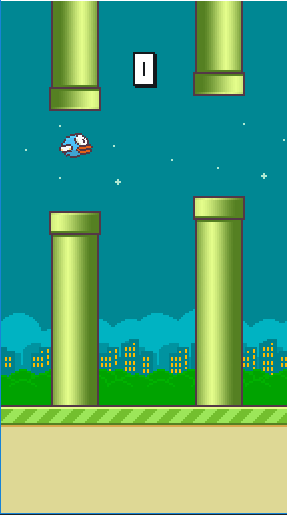
\includegraphics[scale=0.5]{images/flappy.png}
        \caption{Image of FlapPy Bird, reimplementation of Flappy Bird designed for Adam-DQL testing environments}
        \label{fig:52}
    \end{figure}
    
     \begin{itemize}
        \item \textbf{Environment dynamics $s_t$} : $(x_t,\dot{x}_t,\theta_t,\dot{\theta}_t) \in S$, consisting of a state for the agent, following the description presented above. The starting position is $s_0$, a 2D vector $x_0$ and $y_0$ representing the starting position of the bird. The goal is to use bird's flapping ability to cross the gap between pipes. The height of the pipes is uniformly distributed random variable between $[10,90]$. Gap width between upper and lower pipes is uniformly distributed random variable between $[20,60]$.
        \item \textbf{A finite (2) set of actions A}, Flap ($v_y+=9$(m/s)) or do nothing.
        \item \textbf{A reward function} $r=R(s_t,a_t,s_{t+1})$, which is $r=0.1$ for every timestep where the agent doesn't make contact or crosses the pipe. $r=1$ every time the agent crosses a pipe successfully, and $r=-1$ every time the agent makes contact with pipe or ground (thus ending the game/episode).
    \end{itemize}
    
    \subsection{Simplified Tetris}
    
    Consider a tasks which an agent interact with an environment, in this case a simplified version of a classic puzzle game, Tetris. Tetris is a tile-matching puzzle game that involves pieces called Tetriminos. Tetriminos are game pieces shaped like tetrominoes, geometric shapes composed of four square blocks each. A random sequence of Tetriminos fall down the playing field (a rectangular vertical shaft, called the "grid" or "matrix"). The objective of the game is to manipulate these Tetriminos, by moving each one sideways (if the player feels the need) and rotating it by 90 degree units, with the aim of creating a horizontal line of ten units without gaps. When such a line is created, it gets destroyed, and any block above the deleted line will fall. When a certain number of lines are cleared, the game enters a new level. As the game progresses, each level causes the Tetriminos to fall faster, and the game ends when the stack of Tetriminos reaches the top of the playing field and no new Tetriminos are able to enter.
    
       \begin{figure}[H]
        \centering
        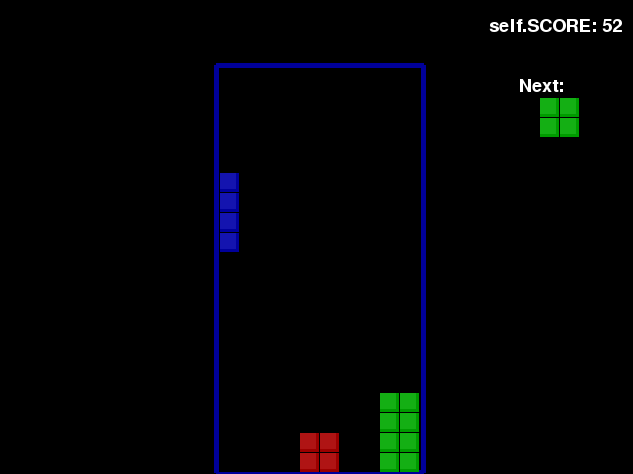
\includegraphics[scale=0.4]{images/tetromino.png}
        \caption{Image of Tetromino, reimplementation of Tetris designed for Adam-DQL testing environments}
        \label{fig:53}
    \end{figure}
      
     \begin{itemize}
        \item \textbf{Environment dynamics $s_t$} : $(b_t,b_{t+1},G_t) \in s$. $b_t$ represents the current falling block at time $t$, and $G_t$ represents the game grid(matrix). For every steps, $b_t$ and $b_{t+1}$ are randomed from 2 tetrimino blocks, "I" (line) block and "O" (square) block. . The game grid is defined to be a matrices of size $20 \times 10$. If a specific point in grid are filled, the next block will be stacked vertically on the grid. For every steps, the position of the current falling block $b_t^x$ and $b_t^y$ have to follow the constraint : $1 \leq b_t^x \leq 10$ and  $1 \leq b_t^y \leq 20$. The goal of the game is to maintain this constrain for the $b_t^y$, which means staying alive by clearing blocks. Blocks are cleared if for $\forall x$ in the grid $G_t^y=1$ (filled).
        \item \textbf{A finite (4) set of actions A}, move right ($b_t^x=b_t^x+1$), move left ($b_t^x=b_t^x-1$), rotate pieces and do nothing.
        \item \textbf{A reward function} $r=R(s_t,a_t,s_{t+1})$, which is $r=100$ for every cleared line, $r=0$ if the agent stays alive and $r=-1$ if the maximum total height of 2 subsequent blocks are bigger than 5.
    \end{itemize}
	
    \section{Experiment Results}
    In order to show and experiment with the newly developed Adam-DQL, an Adam-DQL agent is created and tested for 3 games explained in Section \ref{environment}. The performance data and statistics of Adam-DQL agent will be presented and analyzed in this section. We will try some different configurations for some problem and followed with comparative analysis. In some environments, we may encounter some performance-blocking complication or end-game problems that needs to be properly addressed.
    
    \subsection{Cartpole/Inverted Pendulum}
    
        As a generalization test of the former Q-learning framework, our first task: Cart Pole Problem
        was chosen to access the validity of our new Adam-DQL algorithm. According to \cite{bartosutton}, the problem is considered "solved" after achieving an average reward of 195. This environment is chosen to show the ability of Adam-DQL to learn from \textbf{a pure simulation game}. Where the real tasks is similar to regression tasks. The agent simply needs to approximate the correct equation (representing the equation with neural networks).
        \par 
        On a game like this, once the agent is able to approximate the function, it's not hard to find the appropriate action since the game can easily represented as mathematical equations. This is the reason why this task is the easiest and can be solved in relatively low time. Since each episode has a random
        starting point (initial angle), early episodes ended with an average of 10-20 steps. A target network
        rate of one thousand would make for an extremely slow learning. The rate was changed to ten to
        achieve a higher average reward earlier.
        
        \begin{figure}[H]
            \centering
            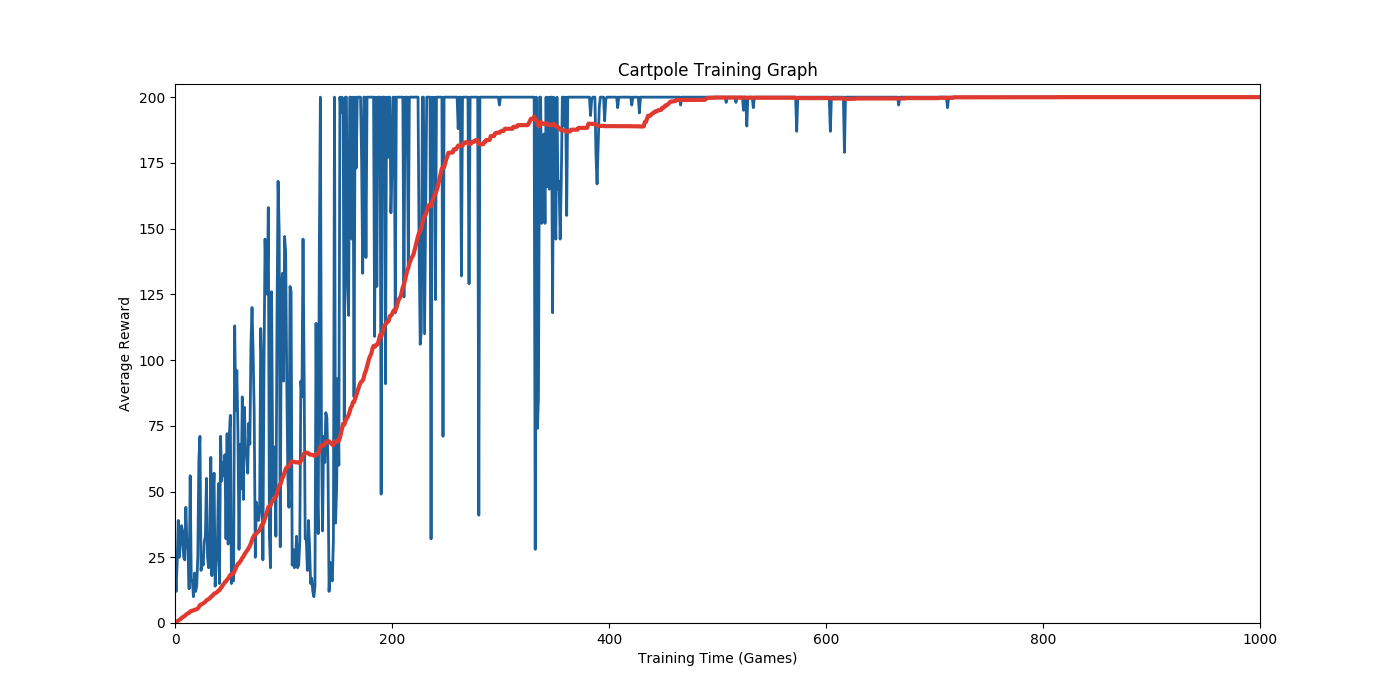
\includegraphics[scale=0.4]{images/Cartpole_Training_Graph.png}
            \caption{The average rewards achieved by the agent alongside it's training time}
            \label{fig:cartpole1}
        \end{figure}
        Figure \ref{fig:cartpole1} shows the training curve of Adam-DQL agent. The red line represents the average reward of the agent while the blue line represents the rolling mean of the agent's performance throughout the training process.
        \par
        One noticeable thing that stands out when we first see in Figure \ref{fig:cartpole1} is the
        oscillation of our agent's performance.This oscillation is due to our
        stochastic optimization procedure, Adam, considering different state-spaces within each step. It is obvious that this is not caused by an instability or diverging oscillations, simply because only the roling mean is oscillating, and not the average reward itself. The average reward itself keeps growing because despite the randomness of early training process, the neural network parameters is still updated towards the global minima, and allows for better policy overtime. Another form of proof for randomness is that the oscillation actually becomes smaller and smaller as the time goes on. This shows that the policy of the agent itself is becoming better, resulting in more consistent gameplay for the latter episodes. 
        
        \begin{figure}[H]
            \centering
            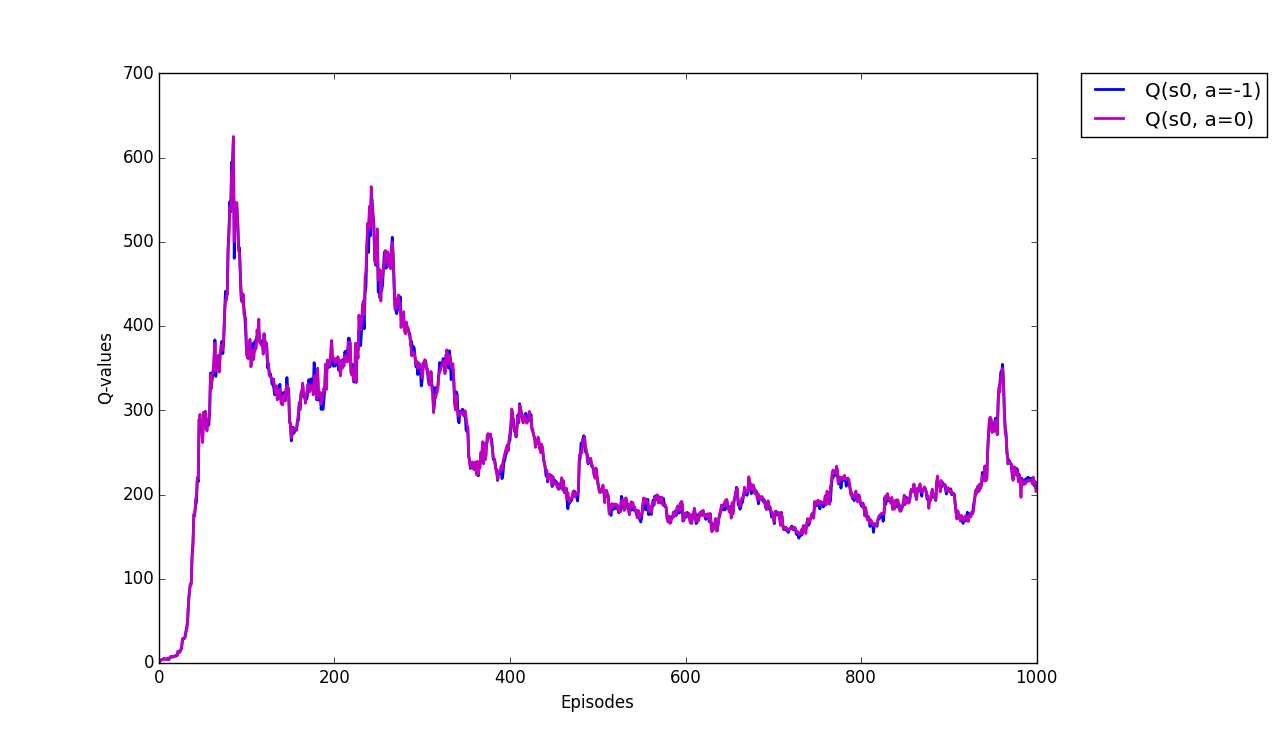
\includegraphics[scale=0.3]{images/qvaluecartpole.png}
            \caption{Q values at the start of every episode}
            \label{fig:cartpole2}
        \end{figure}
        Q-values from both actions are gathered and presented in Figure \ref{fig:cartpole2}. The starting state in each episode is not static. This is obvious because Cartpole problem spawns the cart on a random position, generating different starting dynamics each time. Nevertheless, our Q-network predicts an average of two hundred steps until failure, which is still above the "solved" flag consideration. The fact that these 2 graph almost coincide with each other shows how well Adam-DQL agent generalize or learn the game strategy. Because this 2 Q-values shows how consistent the agent performs despite being thrown on a slightly different starting condition. If the agent is overfitted on the training data, changing the starting condition will resulted in huge drop in agent performance.
        \iffalse
        \begin{figure}[H]
            \centering
            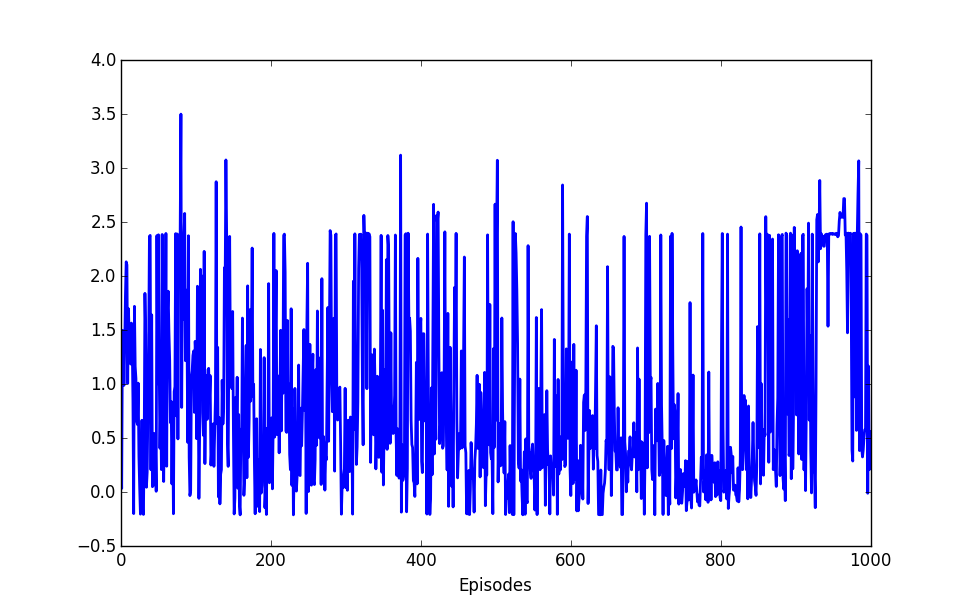
\includegraphics[scale=0.4]{images/value.png}
            \caption{Value function of the Cartpole problem}
            \label{fig:cartpole3}
        \end{figure}
        The value function varies from 0 to 2.5 (the correct value should be around 1). The oscillation is also due to the update-rate and the fact the optimization procedure derives from a stochastic sampling.
        \fi
        \par
         Despite showing steady improvements overtime, to further showcase both the capability and the practicality of Adam-DQL, it is needed to compare the results shown above with a previous work on the same environment. \cite{flappyDL} created an agent using Deep Q-Learning similar to Deepmind's \cite{mnih2015humanlevel} and trained the agent on the same CartPole environment:
         \begin{figure}[H]
             \centering
             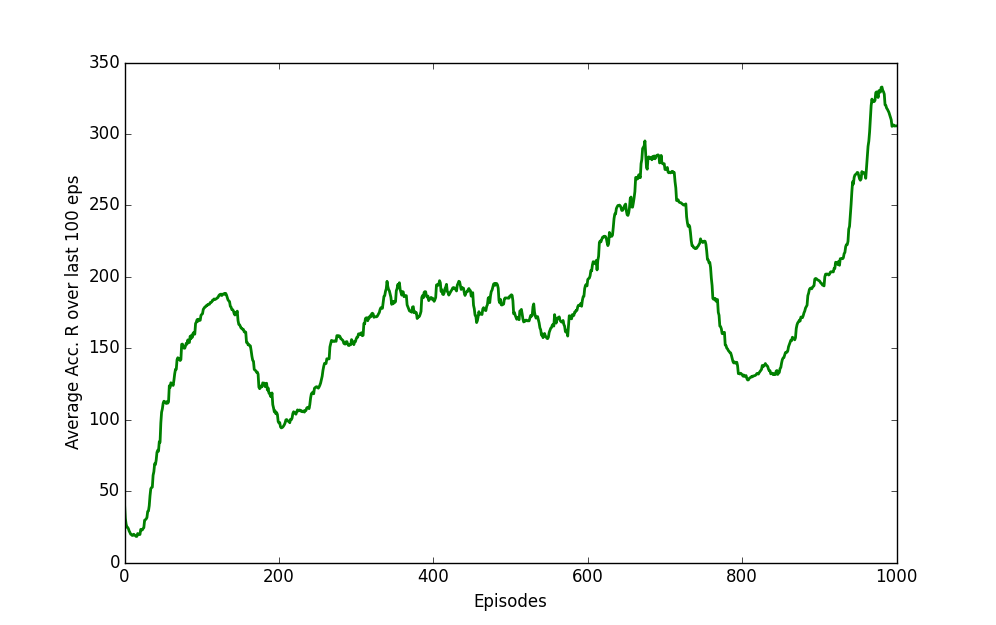
\includegraphics[scale=0.4]{images/rewardcartpole.png}
             \caption[Average Rewards for classiccal Deep Q-Learning Agent]{Average Rewards for classiccal Deep Q-Learning Agent \cite{lillicrap2015continuous}}
             \label{fig:cartpole4}
         \end{figure}
        
        It's clear that compared to Adam-DQL agent result shown in Figure \ref{fig:cartpole1}, classical Deep Q-Learning agent has much more noticeable stability issues on its learning curve. Classical Deep Q-Learning agent oscillates on the reward level, which means it actually has regression in its policy, that is not caused by the stochastic sampling. Adam-DQL agent only oscillates on the standard deviation level, which means that it still plays better overtime, but at the early stages, the quality of play is not as consistent as the later stages. However, classical Deep Q-Learning agent actually plays worse overtime on some intervals, which indicates that the policy itself its becoming worse. 
        \par
        This comes from the fact that Stochastic Gradient Descent (SGD) that is used in classical Deep Q-Learning doesn't account for the gradient historical data. This means, if at a time $t$ the computed gradient actually drives the current approximation away from global minima, the algorithm doesn't have any way to prevent the \textit{bad} gradient ruining the currently better policy. If this happens often, there might be a regression in policy, and thus the agent performance. In this case, it was clear that there's a regression around episode 200 and episode 400, where the agent performance goes downhill and doesn't go back up until few hundred episodes later.
         \par
        This thesis adds 2 additional policy improvement technique for deep Q-learning. However, none of this policy improvement technique will be applied on this problem. Partial training, the first policy improvement technique is inapplicable for this problem, because it is not possible to divide the cartpole problem into smaller subproblems that differs in difficulty. The second improvement, demonstration, is not necessary for this problem. Demonstration tries to help with the problem with a very sparse, hard to achieve reward. Because of how simple this problem is, random exploration is already more than enough to solve this game in a reasonable time. By observing Figure \ref{fig:cartpole1}, it is clear that this problem can be solved in way less than 1000 games. Which is considered instant by modern computing standards. Adding extra human-created transitions is overkill for this problem. 
         
    \subsection{FlapPy Bird}
        
    Our second task: FlapPy Bird is tested and further analyzed on our Adam-DQL agent. This environment is chosen to represent a set of problems where the playing strategy \textit{looks} simple, but it is hard pinpoint precisely, both from mathematical and programming standpoint. It might be possible to create a deterministic algorithm that \textit{somewhat solves} the problem. However it might be impossible to solve it completely. Our Adam-DQL agent is trained and tested on this problem, with the results shown below:
           \begin{figure}[H]
        \centering
        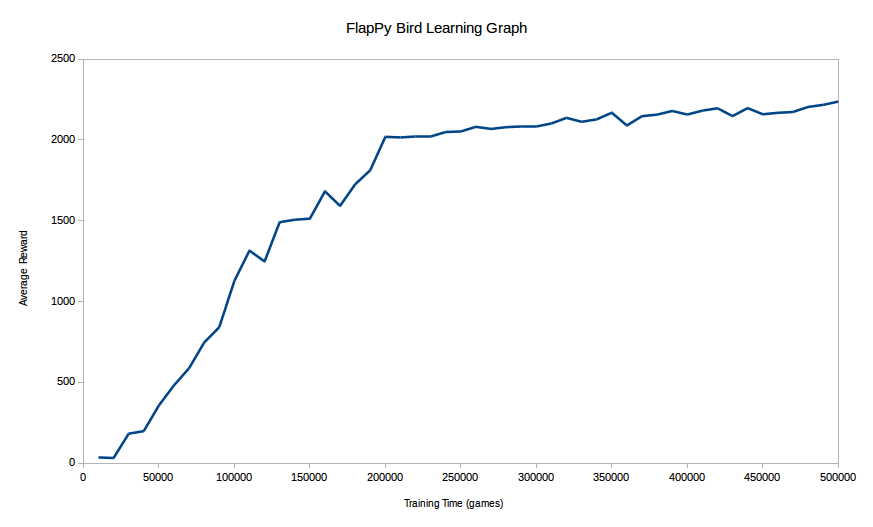
\includegraphics[scale=0.5]{images/flappyreward.png}
        \caption{The average rewards achieved by the agent alongside it's training time}
        \label{fig:flappy1}
    \end{figure}
    In this environment, instead of the global learning parameters $\epsilon=1$ annealed linearly until $\epsilon=0.1$, $\epsilon=0.01$ annealed until $\epsilon=0.001$ is chosen. This is inspired by \cite{flappyDL}. FlapPy Bird is a very fast environment, without a lot of slack time. This means if the agent decided to make a slight mistake, there's a high chance that the episode will end (the agent dies). If every time step, that is $\frac{1}{60}$ sec, $\epsilon=1$ until $0.1$, there's a very high chance that a random action is taken and since the environment only has 2 action, there's a very high chance that the agent will randomly \textit{flap}. If this happens often, which is very likely, the agent will die most of time hitting the pipe at the ceiling. For example, if $\epsilon=0.5$, there's a $\frac{1}{2} \times \frac{1}{2}$ chance that the bird will flap at every timestep. Which means the bird is expected to flap around 15 times in a second. This is way too frequent, and will simply result in the bird staying at the top of the screen. Hence, a really small $\epsilon$ is needed, thus the value $0,01$ annealed linearly to $0,001$ is selected.
    \par
    On this environment, understanding how our neural networks learn and knowing what information is considered \textbf{important} by our neural networks are vital. To achieve this, further analysis to our agents is performed. The output of our two convolutional neural networks is extracted and analyzed.
      \begin{figure}[H]
            \centering
            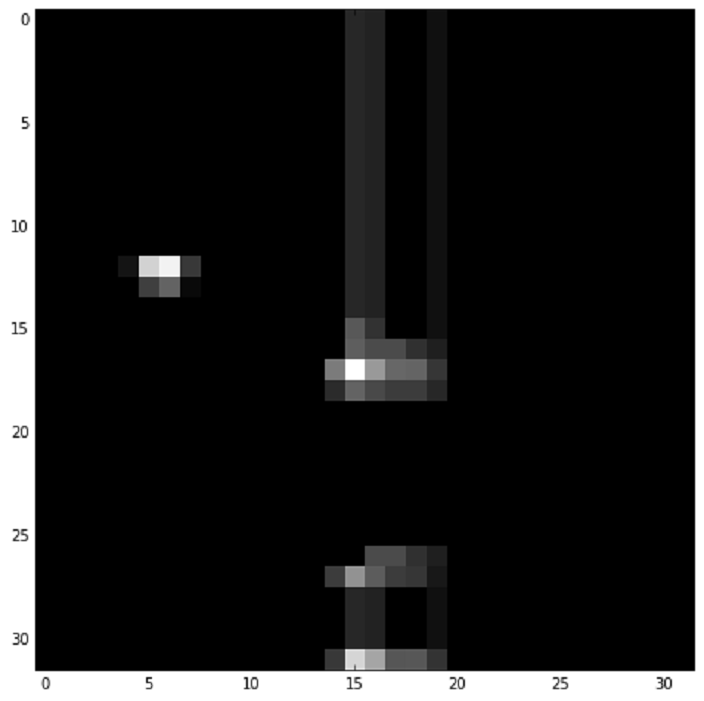
\includegraphics[scale=0.5]{images/layer1.png}
            \caption{The output of the first convolutional layers}
            \label{fig:flappy2}
        \end{figure}
    \begin{figure}[H]
            \centering
            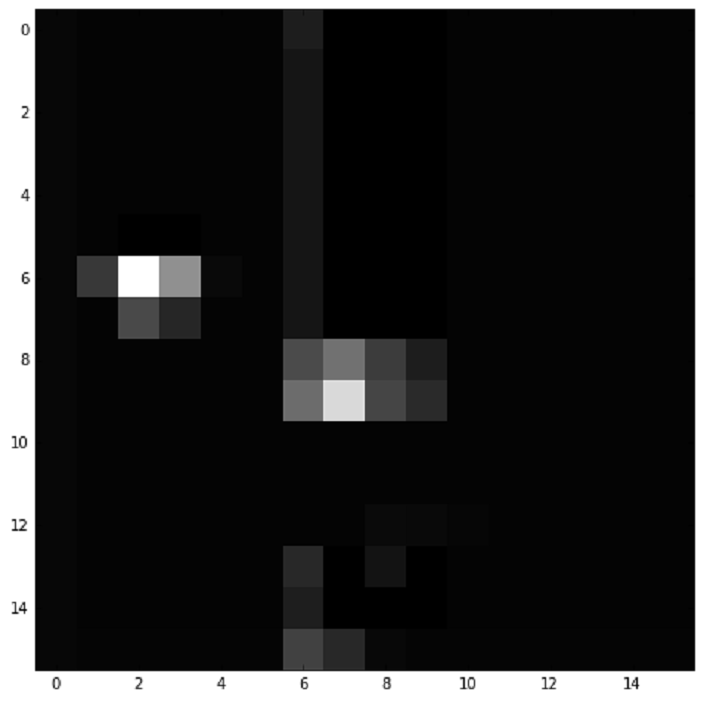
\includegraphics[scale=0.5]{images/layer2.png}
            \caption{The output of the second convolutional layers}
            \label{fig:flappy3}
        \end{figure}
    From Figure \ref{fig:flappy2} and \ref{fig:flappy3}, one can see that the \textbf{important} pixels are the position of the bird and gaps. Furthermore, seeing how the Figure \ref{fig:flappy2} is processed to become Figure \ref{fig:flappy3}, it is clear that the agent is trying to maintain the relative position between the bird and the gap. There's no scientific way to pinpoint how a convolutional neural network "\textit{learns}". However this two image outputs definitely gave some idea about how Adam-DQL agent can learn complex and advanced strategies about this game.
    \par
    Despite showing steady improvements overtime, to further showcase both the capability and the practicality of Adam-DQL, it is needed to compare the results shown above with a previous work on the same environment. \cite{flappyDL} created an agent using Deep Q-Learning similar to Deepmind's \cite{mnih2015humanlevel} and trained the agent on the same FlapPy Bird environment. The results of their work are shown alongside Adam-DQL's score in the table below:
    
        \begin{table}[H]
    \centering
        \label{flappycomparison}
    \begin{tabular}{|l|l|l|}
    \hline
    \# Training episodes     & Deep Q-Learning & Adam-DQL \\ \hline
    10000 (first checkpoint) & 11,6            & 35,1     \\ \hline
    99000                    & 1680,9          & 912,7   \\ \hline
    199000                   & 1026,8          & 1962,6   \\ \hline
    299000                   & 351,06          & 2058,1   \\ \hline
    399000                   & 1006,11         & 2179,4   \\ \hline
    \end{tabular}
    \caption[Average rewards of Adam-DQL FlapPy Bird agent compared to classical Deep Q-Learning agent]{Average rewards of Adam-DQL FlapPy Bird agent compared to classical Deep Q-Learning agent \cite{flappyDL} }
    \end{table}

    Not only that Adam-DQL agent performs better, it also doesn't suffer from regression through training overtime. Adam optimizer, the optimization algorithm for Adam-DQL is amplifying the gradient of the neural network using the first moment(means). This leads to neural network converging or reaching the global minima faster. Adam optimizer also prevents the instability (where the neural networks oscillate around a local minima) by scaling the gradients with second moment(uncentered variance). Because of these reasons, not only our Adam-DQL agent perform better with the same amount of training, it also doesn't suffer from regressions like what happened to the classical Deep Q-Learning that uses Stochastic Gradient Descent (SGD).
    
    As explained in Section \ref{sec:4}, Adam-DQL also implements a technique called \textbf{demonstration}. 100 sets of training data (transitions) are stored into the replay memory $D$ before the training start. This data is taken from human data playing the game for 100 frame sets. The demonstration data is by no means perfect, however this imperfect data will then be replaced by agent's replay memory. This idea is directly taken from \cite{DBLP:journals/corr/abs-1709-10089}, where the suboptimal demonstration data is handled in largely the same way.
    
       \begin{figure}[H]
        \centering
        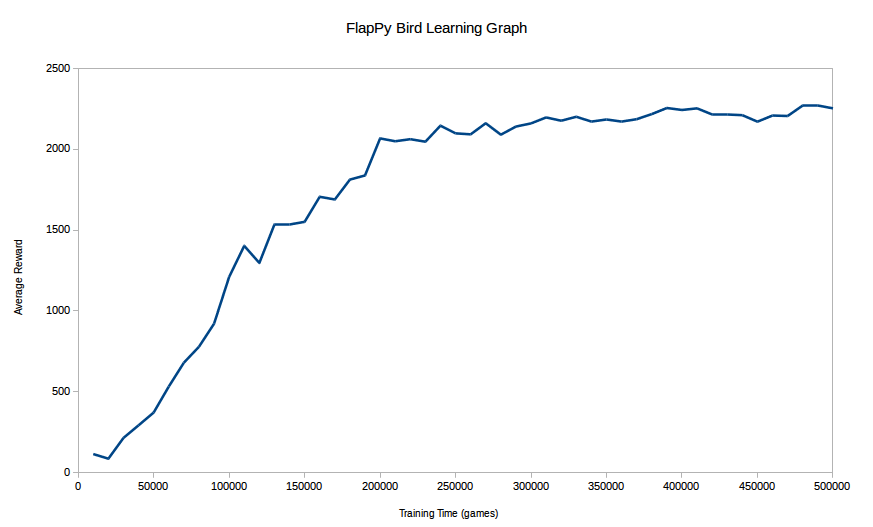
\includegraphics[scale=0.5]{images/flappyrewardemo.png}
        \caption{The reward graph for Adam-DQL with demonstration}
        \label{fig:flappy4}
    \end{figure}
    
    It is clear that there's a huge improvement in the first few training episodes. On the later stages of training process, the improvements over Adam-DQL without demonstration is very subtle. By giving initial "knowledge" to the agent, the agent can start improving pretty fast. Instead of random exploration in the start of the training process, the agent has a basic idea about how the game should be tackled, and explore from there. As explained before, this demonstrations data can be replaced by agent's memory later into the training process, which explain why the improvement on the later stage of the training process is very small. 
    \par
    There's also another improvement that can't be represented by a mere numbers. By kickstarting the agent's learning capability, there's a less chance that the agent will go into a feedback loop (where the agent can't improve because of bad training experience) or diverge catastrophically. Since deepmind proposed experience replay in \cite{mnih2015humanlevel}, there's only a small chance of this divergence actually happening. However, another improvement is certainly a good thing. A tabular comparison of Adam-DQL and Adam-DQL with demonstration is shown below:
    
      \begin{table}[H]
    \centering
        \label{flappycomparison2}
    \begin{tabular}{|l|l|l|}
    \hline
    \# Training episodes     &  Adam-DQL       & Adam-DQL-D \\ \hline
    10000 (first checkpoint) & 35,1            & 114,1     \\ \hline
    99000                    & 912,7           & 1026    \\ \hline
    199000                   & 1962,6          & 1838,7   \\ \hline
    299000                   & 2058,1          & 2141,6   \\ \hline
    399000                   & 2179,4          & 2257,7   \\ \hline
    \end{tabular}
    \caption[Average rewards of "naive" Adam-DQL and Adam-DQL with demonstrations] {Average rewards of "naive" Adam-DQL and Adam-DQL with demonstrations \cite{flappyDL} }
    \end{table}
    
    As with the cartpole problem, it is also not possible to apply partial training to this problem. Partial training requires a problem that can be broken down to subproblems, where each subproblems differ in difficulty. This game relies on putting pipes on different position, which clearly can't be broken down into subproblems, as a pipe with position $x$ isn't a subset of pipe with position $y$. Thus partial training won't be applied for this problem, despite the game being relatively hard.
    
    \subsection{Simplified Tetris}
    Our final task: simplified Tetris, is tested and analyzed on Adam-DQL. This environment is selected to represent a problem that is both hard to model, verify or even approximate \cite{DBLP:journals/corr/cs-CC-0210020}, which is why Tetris is considered NP-Complete. Not only it's hard to approximate a solution for Tetris, it's also hard to verify whether that solution is actually correct or not. For this reason, Tetris is considered an untouched problem in reinforcement learning, as it's hard to justify every actions and reward. Some researchers have attempted to solve Tetris as a reinforcement learning problem, albeit without a good results. This is why, this thesis is using a simplified version of tetris, instead of full version of Tetris with 6 type of tetrominis. This reduce the complexity of tetris to a reasonable degree. To further indicate how hard tetris is, below is the learning graph of "naive" Adam-DQL (without any policy improvement technique):
    
     \begin{figure}[H]
        \centering
        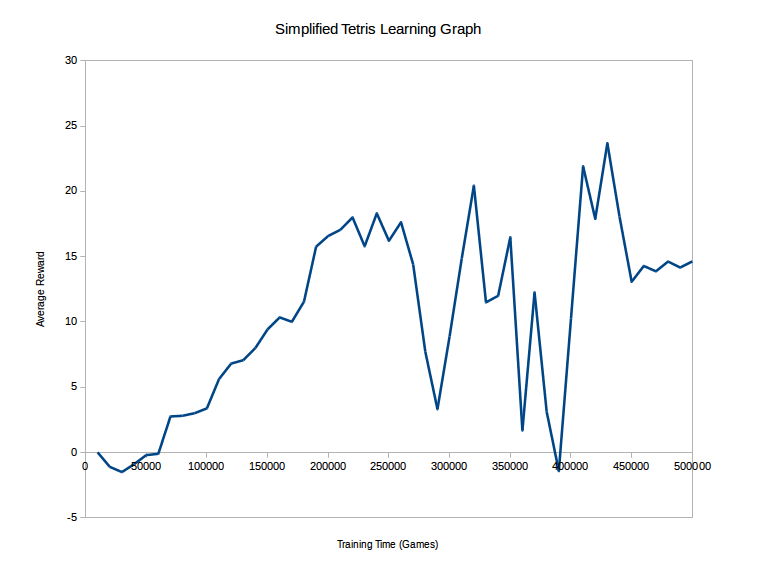
\includegraphics[scale=0.5]{images/tetrisreward.png}
        \caption{The average rewards achieved by the agent alongside it's training time}
        \label{fig:tetris1}
    \end{figure}
    
    It's really clear that the agent struggles to solve the problem. The reward graph oscillates extremely, indicating that there's no clear policy that the agent can infer from the environment. The reward at the end of the training is also way less than $100$, which indicates that the agent can't even clear $1$ line consistently for every game. Fortunately, there's a clear explanation about why this happened, and it has to do with the idea of Q-learning itself.
    \par
    From Chapter \ref{sec:4}, the bellman equation is defined as follows:
    \begin{equation*}
         Q_{i+1}(s,a)=\E[r+\gamma\max_{a'}Q_i^*(s',a')]
    \end{equation*} 
    Note that to update $Q(s,a)$, Q-learning relies on a term $r$, which is the reward term. To put it simply, if the agent doesn't get any reward in 2 subsequent states, $Q(s',a')=Q(s,a)$ and $r=0$, which means $Q(s,a)=0+Q(s',a')=Q(s,a)$. This also applies to deep Q-learning, where the neural network won't be able to learn unless it receives some rewards. At the start of the neural network, all the weights and parameters are initialized randomly, and $\epsilon$ is initialized to 1. This means before training, neural network is basically doing a random exploration. 
    \par
    Tetris is a different "type" of problem from FlapPy Bird and Cartpole. The later represents \textbf{reflex-based} games, where it relies on human reflexes combined with some strategy, while Tetris is a \text{strategy-based} game. This is really important, because on a game that relies on reflexes, using a random exploration might resulted in a reward. For a strategy game, an agent might need to do a set of planned strategy just to get a reward. By not getting any reward, the agent basically does a random exploration, but since the game needs a strategic planning, it will never get a reward, and so on. On robotic terms \cite{DBLP:journals/corr/abs-1709-10089}, problem like this is said to have \textbf{sparse} rewards.
    \par
    Deepmind's original deep Q-learning also struggles from the same problem \cite{mnih2015humanlevel}. While some games performed amazingly, game with sparse rewards struggles to even get a single reward. However, This doesn't mean that deep reinforcement learning in general is impossible for these kind of environments, as there's a possible solutions for this phenomenon. The main problem is that the agent can't get a reward, which means by giving some sort of help, the agent can start learning, and in the end, strategize for itself.
    \par 
    This is where our first policy improvement technique comes in, partial training, which is aimed to reduce the complexity and strategy needed to get a reward, is applied to our simplified Tetris environment. The environment is broken down into 2 subproblems, the first subproblem is a Tetris with only 1 tetrominis, the "O"(square) block. Randomly putting the square block into the grid has a reasonable chance clear a line, which means that the agent might receive a reward just by playing randomly. This subproblem is definitely easier to solve, and it helped our neural network to start learning. After trained to some extent, this agent is now much better prepared to solve the full environment with two blocks.
    
    
     \begin{figure}[H]
        \centering
        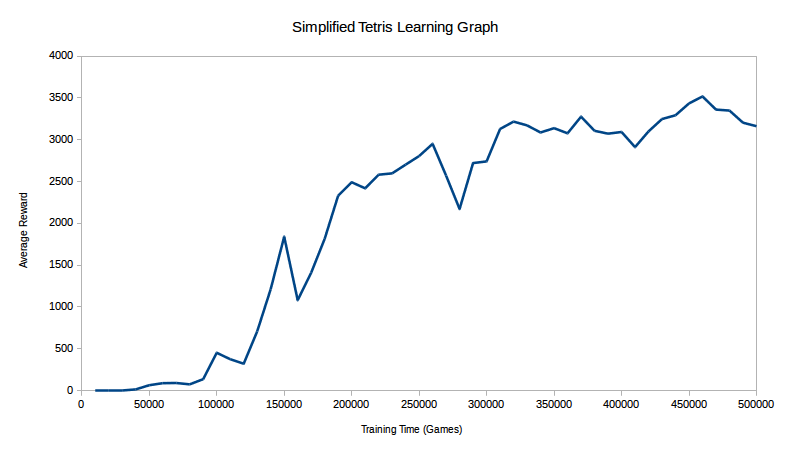
\includegraphics[scale=0.5]{images/tetrisreward2.png}
        \caption{TThe reward graph for Adam-DQL with partial training}
        \label{fig:tetris2}
    \end{figure}
    
    It is clear that from Figure \ref{fig:tetris2}, the difference made by implementing partial training is night and day. Not only the agent learn much more steadily (without extreme oscillation), the agent now can achieve around 3000-3500 reward points. This means our agent can clear on average 30 lines a game, which is a huge improvement from standard Adam-DQL.
    \par
    Demonstration, our second policy improvement technique is also applied and tested for Tetris environment. Demonstration tries to help the agent to get a reward with a different way. Instead of reducing the complexity of the problem, demonstration is aimed to give some initial strategy by feeding human-created transitions into agent memory. 100 frames of human-created transitions are stored into replay memory $D$ before the training process starts.
    
    \begin{figure}[H]
        \centering
        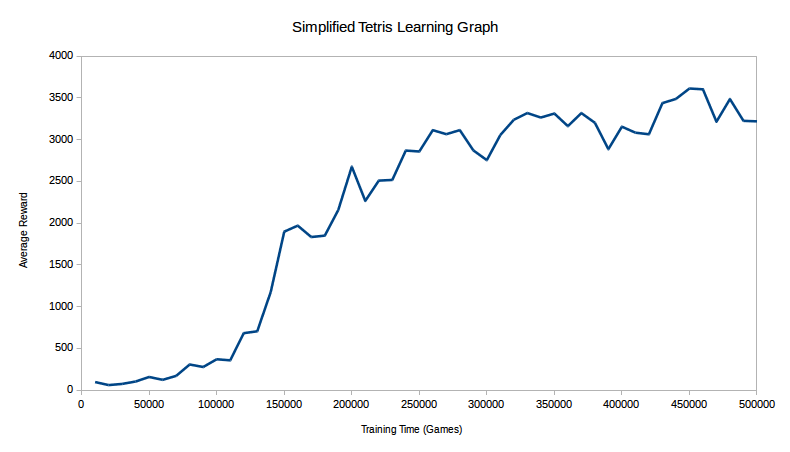
\includegraphics[scale=0.5]{images/tetrisreward3.png}
        \caption{The reward graph for Adam-DQL with partial training and demonstration}
        \label{fig:tetris3}
    \end{figure}    
    
    Clearly, from Figure \ref{fig:tetris3}, demonstration seems to help "lift" the early part of the training process. This synergizes with the idea that it tries to help initial training process. However, as with FlapPy Bird, demonstration doesn't seem to help with the later stages of training process. As it has almost identical reward as Figure \ref{fig:tetris3}. Again, this comes from the fact that the human-created transition is replaced after several training episodes.
    \par
    These 2 improvements on Adam-DQL dont simply make tetris completely solvable with Adam-DQL, however. On the later stages of training process, Figure \ref{fig:tetris2} and \ref{fig:tetris3} indicate that the performance of the agent got stuck around 3000 mark. From our extensive testing, this performance doesn't grow anymore with more training time. Which indicates there's something preventing the agent from learning more. From our analysis, this can be caused by 2 things:
    \begin{enumerate}
        \item The game has a really sparse rewards, which means that most of the time, the agent is gonna get 0 or even negative reward. Adam-DQN uses ReLU (rectified linear unit) which is defined as $\phi(x)= max(0,x)$. 
        Assume a very simple loss function $L(y)=\phi(\hat{y})-y$ is used, for a parameter $\theta_n$, there's only 2 possible gradient value:
        \begin{equation*}
            \frac{\partial L}{\partial \theta_n}=\delta_n=
            \begin{cases}
            1 & \theta_n \geq 0\\
            0 & \theta_n < 0
            \end{cases}
        \end{equation*}
        which simply means, if the value of a neuron is smaller than 0, the gradient will be 0 and the parameter won't be updated. Since  $\phi(0)$ is also 0, this will result in a dead neuron, which means this neuron won't be able to learn anything anymore.
        \item The reward for an action in Tetris is usually very delayed. Adam-DQL uses discounted future reward, which means a reward given on the 1000 timesteps ahead for example, is discounted by discount factor $\gamma^{100}$. This is a structural problem which is harder to solve, because the standard value for $\gamma$ is $0.99$, which is already really close to 1. Still, $0.99^{100}=0.366$, which is relatively small. This nullifies the value of that action to the final reward, making it harder for the agent to pinpoint which action produces a reward.
    \end{enumerate}
    
    This 2 problem is currently unsolved for Adam-DQL agent. However, this can be a guidance and idea for further research.
    
    

%=================================CHAPTER VI=========================================

\chapter{CLOSING}
\thispagestyle{fancy}

%====================================================================================
	\section{Conclusions}
	    \iffalse
	    First, we discuss how to derive the governing equations of fluid dynamics related to blood flow. In section 2, we start from an introduction to Reynold's transport theorem, and we demonstrate how it relates to the derivations of the conservation law equations. Furthermore, the influence of the assumptions on the equations is also discussed.
	    \par
	    Second, we discuss how to derive the SPH numerical schemes for the governing equations. In section 3, we first discuss the underlying idea of SPH approximations. Then, we discuss about the properties of the smoothing functions and the choices of the smoothing functions. After that, we derive the SPH numerical schemes and discuss about time integration.
	    \par
	    Last, we discuss how to develop the code and the graphical simulation. In section 4, we first discuss about the boundary models. After that, we discuss how to achieve a steady flow in the numerical simulation. Then, we present the design of the graphical simulation. In section 5, we discuss about the results and implementation. We also evaluate the performance of the code, and we describe ways to optimize performance.
	    
        The governing equations of fluid dynamics related to blood flow in the artery has been successfully derived. The Reynold's transport theorem is used to derive the conservation laws equations. The result is the incompressible Navier-Stokes equation with constant viscosity. \par
	    We use the SPH method to numerically solve the governing equations. We discussed the underlying idea of SPH approximations. We discussed about the properties of the smoothing functions and the choices of the smoothing functions. We derived equations to easily evaluate the derivatives of the smoothing functions, and we presented proofs that the chosen smoothing functions satisfy the properties. We developed the numerical schemes by directly discretizing the Navier-Stokes equation using the SPH method. \par
	    The code and the graphical simulation are implemented within the MATLAB R2013a programming environment. The user interface is created using the MATLAB's GUIDE. The performance analysis results showed that preallocation significantly affects the run time. The boundary treatment method together with the inlet and outlet boundary conditions are used to achieve a steady flow. The numerical simulation results showed that a steady flow has been successfully achieved. The flow in the pulsating artery case is pulsatile. In the pulsating stenosed artery case, the pressures of the particles at the narrowed part are higher than the nonpulsating stenosed artery case. 
        \fi
        
        A new deep reinforcement learning model for video games has been successfully developed. Deepmind's Deep Q-Learning and Adam optimizer are combined to allow deep reinforcement learning to be used in a more complex video games. The result is Adam-DQL, a deep reinforcement learning model that handles immense state spaces extremely well. To further improves stability, a new training/improvement policy on deep-reinforcement learning is required. Partial training, a technique based on the idea of kickstarting an agent to experience more rewards/punishment is developed. A similar technique proposed for robotic environment, called demonstrations, is also applied on Adam-DQL. 
        \par
        Adam-DQL agent is created within Tensorflow environment on top of Python 2.7.13. Several framework architectures are considered and tested. Testing environment based on video games are proposed and used to test Adam-DQL's capability to solve different type of video games. Adam-DQL agents are tested on 3 games, with different type and complexity. The results is then plotted and compared to classical deep Q-Learning. Adam-DQL shows superior results from both training speed and reward standpoint. On some games, Adam-DQL even shows really drastic improvements. Demonstration helps Adam DQL agent to start improving pretty fast, and combined with partial training, Adam-DQL agent can solve harder games that's rarely touched by deep reinforcement learning before.   
%====================================================================================
	\section{Future Works}
		\iffalse
		The computational cost of the code is still expensive. The SPH method's computational complexity significantly depends on the algorithm used for nearest neighbor search. In this thesis, the exhaustive search is used. The exhaustive search is very easy to implement, but it is the most computationally expensive nearest neighbor search algorithm. The computational complexity of the exhaustive search is $O(N^2)$, where $N$ is the number of particles. Thus, applying a better nearest neighbor search algorithm such as neighbour lists is strongly recommended. \par
		To simulate the behavior of solid boundaries, the use of appropriate boundary treatment methods is essential. Using the boundary treatment method described in section 4.1.2, we found that we need a smaller time step for the pulsating artery case to prevent penetration. A smaller time step implies more expensive computational cost. Hence, an adaptive time step approach is suggested. Another approach is to mathematically solve for the intersection point between the straight trajectory of the particle and the boundary equation. Then, the direction of the particle is directly inverted to simulate the collision. \par
	    In this thesis, blood is assumed as a Newtonian fluid. As described in section 2.3, the Newtonian fluid assumption is valid for blood in larger arteries such as the coronary arteries. Hence, it is suggested that the model is further developed for blood in smaller arteries where the non-Newtonian behavior is significant. Furthermore, the model can also be further developed by taking into account the elasticity of the blood vessel. \par
		The developed model can also be used for wider applications. It is suggested that the model is used for estimating the risk of artery wall rupture. The graphical user interface can also be improved. When a pop-up message is displayed or when the progress bar is displayed, the user interface should be disabled. Furthermore, the parameter to determine the degree of stenosis has not been implemented in the user interface yet. It is suggested that the relationship between the parameter to determine degree of stenosis and the time step required to prevent penetration is also determined.
		\fi
		Adam-DQL agent in this thesis are specifically developed for pyGame environment. To allow applications in wider variety of games, it is suggested that the agent are created with any video games environment in mind. The use of faster language (C++) is also recommended as performance is critical for video games. The software framework in general can also be improved, by converting the general structure from a reusable class to a shared libraries, that will allow easier testing and distribution for further research. Furthermore, a stronger hardware for training is strongly recommended.
		\par
		In this thesis, a simplified Tetris environment, consisting of only 2 blocks is used. Based on the idea of training the agent on the simplest subproblems first, further training by using partial training for the rest of the Tetris blocks in this specific order: $\{L,T,S\}$, a fully performing Tetris agent can be developed. There's also 2 unsolved problem for this environment, which is blocking the further improvement of the Tetris environment, which hopefully can be solved in the future.
		\par
		The developed Adam-DQL model can also be used for wider applications. Despite being designed specifically for video games, the model itself can be used for almost every reinforcement learning tasks. For example, by feeding an image of stock prices movements to the neural network, an automated stock training agent can be developed. Furthermore, Adam-DQL agents can also be used in robotic tasks as it combines movement (action) and vision (states). 
		

%=================================REFERENCES========================================
\fancyhead{}
\renewcommand{\headrulewidth}{0pt}
\fancyfoot{}
\rfoot{\thepage}
\thispagestyle{fancy}
\bibliographystyle{unsrt}
\renewcommand{\bibname}{\large REFERENCES}


\bibliography{References}
\addcontentsline{toc}{chapter}{REFERENCES}
\pagebreak

%==================================APPENDIX=========================================
	\appendix
	\addcontentsline{toc}{chapter}{APPENDIX}
	\appcaption{Appendix A\hspace{0.5cm}Code}
	\thispagestyle{fancy}
	\setcounter{page}{1}
	\renewcommand{\thepage}{A-\arabic{page}}
	\begin{singlespace}
	\chapter*{\large Appendix A \hspace{0.5cm} Code }
\thispagestyle{fancy}

	
\lstinputlisting[language=Python, caption=Adam Deep Q-Learning]{code/Adam-DQL.py}
\lstinputlisting[language=Python, caption=FlaPy Bird Environment]{code/flappy.py}
\lstinputlisting[language=Python, caption=Cartpole Environment]{code/cartpole.py}
\lstinputlisting[language=Python, caption=Simplified Tetris Environment]{code/tetris_fun.py}






























	\end{singlespace}
%	\clearpage
%	\pagenumbering{arabic}
%	\renewcommand{\thepage}{B-\arabic{page}}
%
%	\appcaption{Lampiran B\hspace{0.5cm} Contoh Pengerjaan Prosedur Hibridisasi AG-SIB}
%	\begin{singlespace}
%	\include{appB}
%	\end{singlespace}

\end{document}